%\documentclass[unicode,master]{scutthesis} % 草稿封面,硕士则添加选项master,博士则去掉。使用正式封面时注释该行
\documentclass[unicode,master,pdfcover]{scutthesis} %   % 论文正式封面,pdfcover为可选项,终稿再添加,使用草稿封面时注释该行
\usepackage{fontspec,color,array,longtable,graphicx} 
%%%%%%%%%%%%%%%%%%%%%%%%%%%%%%%%%%%%%%%%%%%%%%%%%%%%%%%%%%%%%%%%%%%%%%%%%%%%%%%%%%——by MCH
%编译范围
%\includeonly{chapter03}
%参考文献设置
\usepackage[backend=biber,style=gb7714-2015,gbalign=gb7714-2015,gbpub=false,gbnamefmt = lowercase]{biblatex}
\addbibresource[location=local]{MyLibrary.bib} % 如果在其他盘,改为相对路径。比如F盘,改为:F/MyLibrary.bib
\addbibresource[location=local]{mybibfile2.bib} % 无论什么来源的bib文件,只要由参考文献的BibTeX组成,都可以使用此模板。参考文献的BibTeX获取方法可百度
%页眉页脚设置
\usepackage{fancyhdr}
\usepackage{listings}
\usepackage{xunicode}
\usepackage{multirow}
\renewcommand{\lstlistingname}{列表}
\pagestyle{fancy}
\fancyfoot[C]{\headfont\thepage}
\renewcommand{\chaptermark}[1]{\markboth{\chaptername\ #1}{}}
\renewcommand{\sectionmark}[1]{\markright{\thesection\ #1}}
\fancyhead[RE]{}
\fancyhead[RO]{}
\fancyhead[LE]{}
\fancyhead[LO]{}
\fancyhead[CO]{\headfont{\leftmark}}
\fancyhead[CE]{\headfont{华南理工大学硕士学位论文}}% 
\renewcommand{\headrulewidth}{1.5pt}
\renewcommand{\footrulewidth}{0pt}
%%%%%%%%%%%%%%%%%%%%%%%%%%%%%%%%%%%%%%%%%%%%%%%%%%%%%%%%%%%%%%%%%%%%%%%%%%%%%%%%%%
\usepackage[unicode=true,bookmarks=true,bookmarksnumbered=true,bookmarksopen=false,breaklinks=false,pdfborder={0 0 1},backref=false,colorlinks=true]{hyperref}
\hypersetup{pdftitle={基于RISC-V的DSP微处理器及SoC实现与研究},
	pdfauthor={陈若晖},
	pdfsubject={华南理工大学硕士学位论文},
%%	pdfsubject={华南理工大学博士学位论文},
	pdfkeywords={\LaTeX{};\LaTeX{}},
%%		linkcolor=black, anchorcolor=black, citecolor=black, filecolor=black, menucolor=black, urlcolor=black, pdfstartview=FitH}% 黑白,提交版
	linkcolor=blue, anchorcolor=black, citecolor=red, filecolor=magenta, menucolor=red, urlcolor=magenta, pdfstartview=FitH}% 彩色

\makeatletter
%%%%%%%%%%%%%%%%%%%%%%%%%%%%%% LyX specific LaTeX commands.
\providecommand{\LyX}{\texorpdfstring%
	{L\kern-.1667em\lower.25em\hbox{Y}\kern-.125emX\@}
	{LyX}}
%% Because html converters don't know tabularnewline
\providecommand{\tabularnewline}{\\}
\makeatother
\begin{document}
	%%%%%%%%%%%%%草稿封面设置%%%%%%%%%%%%%使用“正式封面”时不需要理会这部分
	\title{基于RISC-V的DSP微处理器及SoC实现与研究}	
	\author{陈若晖}	
	\supervisor{指导教师:赖晓铮\ 教授}	
	\institute{华南理工大学}	
	\date{2022年3月31日}
	%%%%%%%%%%%%%%%%%%%%%%%%%%%%%%%%%%%%%
	\maketitle	
	\frontmatter	%此后为罗马数字页码,页面类型为plain
	\chapter{摘\texorpdfstring{\quad}{}要}

	计算机体系结构在过去几十年的计算机发展历史中不断的演化更替,催生出了种类繁多的计算机指令集架构。现今存在着多种主流的计算机指令集架构,如x86、ARM、MIPS、OpenRISC等。迈入21世纪以来,简洁明快的RISC指令集开始成为微处理器设计的主流,而现存的RISC指令集如MIPS、SPARC、ARM等则或多或少存在着历史遗留的缺陷,为了解决这一问题,伯克利大学在2010年启动了第五代的RISC项目,设计了全新的RISC-V指令集架构,其特点是免费开源以及提供了许多现代化微处理器设计的技术特性,包括可选的扩展指令集、自定义指令功能以及用户与特权架构分离等。基于以上的特性,RISC-V微处理器正迅速占据着除桌面型微处理器以外的市场。与此同时,随着微处理器架构复杂程度的不断提升,对微处理器进行设计的工具与框架也面临着随之而来的效率与生产力的挑战,传统的集成电路设计工具与方法学如基于Verilog/SystemVerilog的瀑布设计模式开始变得捉襟见肘。随着基于敏捷硬件设计方法学设计工具如Chisel、SpinalHDL的兴起,基于高级编程语言并吸收了软件工程学方法的各类新兴硬件设计工具及框架开始逐步被学术界以及工业界所接受。本文将介绍基于RISC-V的开源面向嵌入式场景的DSP微处理器及其SoC及其设计,其实现了RV32GCP指令集架构,在性能上能够对标ARM专为嵌入式设备设计的微处理器Cortex-M3。该微处理器能够填补当前国内对于开源RISC-V DSP微处理器的空白。同时,本文还介绍用于构建该微处理器的硬件设计与验证框架PyHCL,PyHCL是第一款基于Python的RTL级硬件构造语言,相比于Chisel,PyHCL提供更为简单易用的用户接口,较短的学习曲线以及完整的Python特性支持。其效率要优于Chisel,且相比仅支持单元测试的Chisel,PyHCL具有完整的验证环境支持,包括单元测试、功能测试、差分测试等。本文由两大主要部分组成:一是基于RISC-V的DSP微处理器,二是敏捷硬件设计工具PyHCL,在本文最后也会阐述用于本微处理器验证过程中所使用的PyHCL验证方法,并介绍用于本文实现的微处理器验证所使用的基于多级验证环境的差分测试框架。

\keywordsCN{计算机体系结构;微处理器;RISC-V;敏捷硬件设计;Python}

\chapter{Abstract}

	Computer architecture has evolved over the past decades of computer development history. Therefore, a wide variety of computer instruction set architectures have been created in the past few decades. Today, there are several mainstream instruction set architectures, such as x86, ARM, MIPS, OpenRISC, and so on. Entering the 21st century, the soncise and simple RISC instruction set has become the mainstream of microprocessor design, while the existing RISC instruction sets such as MIPS, SPARC, and ARM have more or less defects left over from history. In order to solve this problem, Berkeley University launched the fifth-generation RISC project in 2010, designed a new RISC-V instruction set architecture, which is characterized by free open source and provides many technical features of modern microprocessor design, including optional extensions Instruction sets, custom instruction capabilities, and separation of user and privilege architectures. Based on the characeristics mentioned above, RISC-V microprocessors are rapidly occupying the market other than desktop microprocessors. At the same time, with the continuous improvement of the microprocessor architecture complexity, the tools and frameworks for designing microprocessors also face the challenges of efficiency and productivity. Traditional integrated circuit design tools and methodologies such as The waterfall design pattern based on Verilog/SystemVerilog is starting to become stretched. With the rise of design tools based on agile hardware design methodologies such as Chisel and SpinalHDL, various emerging hardware design tools and frameworks based on high-level programming languages ​​and absorbing software engineering methods have gradually been accepted by academia and industry. This article will introduce the design of a RISC-V open source DSP embedded microprocessor and SoC, it implements the RV32GCP instruction set, which can match the performance of the embedded microprocessor design by ARM: Cortex-M3. The microprocessor can fill the gap for open source RISC-V DSP microprocessors. At the same time, this paper also introduces the hardware design and verification framework PyHCL used to build the microprocessor. PyHCL is the first RTL-level hardware construction language based on Python. Compared with Chisel, PyHCL provides a simpler and easier-to-use user interface, short learning curve ,and full Python feature support. The efficiency of PyHCL is better than Chisel. Compared to Chisel, which only supports unit testing, PyHCL has complete verification environment support, including unit testing, functional testing, differential testing, etc. This paper consists of two main parts: one is the design of the DSP microprocessor based on RISC-V, and the other is the agile hardware design tool PyHCL. At the end of this paper, the PyHCL verification method used in the verification process of this microprocessor will be described. Also, we would introduce the differential test framework based on the multi-level verification environment used for the verification of the microprocessor.

\keywordsEN{Computer Architecture; Microprocessor; RISC-V; Agile Hardware design; Python} % 中英文摘要
	%%%%%%%%%%%%%%%%%%%%%%%%%%%%%%%%%%%%%%%%%%%%%%%%
	% 目录、表格目录、插图目录这几个字本身的大纲级别是一级的,即和章名有相同的字号字体。目录表的内容通过titletoc宏包在。cls文件设置了。
	\tableofcontents	%目录
%	\listoftables	%表格目录(可选)
%	\listoffigures	%插图目录(可选)
	%%%%%%%%%%%%%%%%%%%%%%%%%%%%%%%%%%%%%%%%%%%%%%%%%
%	\include{symbols}	% 符号对照表(可选)
%	\include{abbreviation} 	% 缩略词	
	
	\mainmatter %此后为阿拉伯数字页码
	
    %%%%%%%%%%%%%%%%%%%%%%%%%%%%%%%%%%%%%%%%%%%%%%页眉页脚设置 ——by MCH 
    \fancypagestyle{plain}{
    	\pagestyle{fancy}
    }	% 每章的第一页会默认使用plain,没有页眉。通过重定义plain为fancy解决
    \pagestyle{fancy}	%设置页眉页脚为fancy
    %%%%%%%%%%%%%%%%%%%%%%%%%%%%%%%%%%%%%%%%%%%%%%分章节,结合导言区的\includeonly命令可仅编译部分章节,编译时不用切换界面,直接在相应章节编译即可。
	\chapter{绪论}
%
\section{RISC指令集架构与RISC-V}
\subsection{研究背景}

指令集架构(Instruction Set Architecture,ISA)是计算机体系结构中,介于微处理器架构(Microarchitecture)与操作系统之间的接口。指令集架构用于抽象微处理器底层的具体硬件实现以提供给操作系统一个简洁的硬件接口来管理计算机硬件系统。最早的指令集架构可以追溯到1964年IBM发布的IBM System/360指令集架构,并实现在同时发布的IBM 360计算机族当中[1]。IBM System/360的设计初衷是为了给IBM 360计算机族中不同型号的微处理器为操作系统提供一个统一的接口,而无需针对不同的微处理器实现而设计不同的接口。

指令集架构经过几十年的发展,现今已经出现了众多主流的指令集架构。下面对最为流行的三种指令集架构进行介绍:

\begin{enumerate}
	\item 	x86。x86是1978年由Intel公司推出的著名复杂指令集计算机(Complex Instruction Set Computer,CISC)指令集架构,作为桌面型个人计算机市场最主流的指令集架构,其成功来源于推出时对IBM计算机的兼容以及较好的向后兼容性。然而,从现今的眼光看来,x86已经变得臃肿而复杂,自发展至今到现在x86已经添加了大量的复杂指令。截止2015年,x86已经拥有1300多条指令,大量的寻址模式,大量的特殊寄存器以及多种转换寻址的策略。同时,x86也有一些固有的缺陷,如贫瘠的寄存器数目以及多种隐式的技术特性,包括隐式的条件编码以及预测移动等,这在高性能的微处理器中是难以实现的[2]。
	\item	ARM。ARM是1985年由ARM Holding公司开发的精简指令集计算机(Reduce Instruction Set Computer,RISC)指令集架构。ARMv7是ARM的32位版本,2011年发布了基于64位的ARMv8版本。ARM由于其低功耗、低成本的特性,被广泛应用于嵌入式系统当中。在RISC-V发布前,ARM在嵌入式市场占据绝对主导地位,且在大多数的消费电子设备如便携式设备以及电脑外设等当中占有大部分的市场。然而,ARM也存在着不少的缺点,如混合的特权级以及用户级架构、独立的压缩指令集Thumb等。
	\item	MIPS。MIPS是1985年由MIPS科技公司开发的RISC指令集架构。MIPS是最经典的RISC架构,其影响了后续大多数的RISC指令集架构的设计思想。MIPS采用加载-存储的存储器访问架构,这意味着只有加载以及存储两种内存指令,其他所有的算术操作都是在寄存器上进行,这种设计降低了指令集以及实现硬件的复杂性,在编译器技术提升的基础上,可以促进更为简单的流水线处理器实现。虽然MIPS简单易行设计使得在学术领域青睐有加,但是该指令集架构还是有几个技术上的缺陷使得它对于高性能的实现来说不具有吸引力,如固定的分支延迟间隙(Delay Slot)、对动态链接的支持非常糟糕、乘除法使用了特殊的架构寄存器等等。
\end{enumerate}

从上述三个典型的主流指令集的现状可以看出,目前的指令集架构发展趋势主要有以下方面:

\begin{enumerate}
	\item RISC指令集占据主导地位。进入21世纪以来,仍在广泛流行的CISC指令集仅剩下x86。同时,随着AMD K2微处理器架构发布以来,所有的Intel的乱序执行的处理器引擎都会动态的将x86的指令转化成内部的更接近于RISC风格的微指令执行。x86芯片的出货量自2011年达到峰值以来,每年下降近10%,而采用RISC处理器的芯片出货量则飙升至200亿。
	\item 主流指令集架构囿于设计年代久远而逐渐暴露历史遗留缺陷。x86随时间不断膨胀而变得臃肿的指令集,ARM低效的压缩指令集Thumb,MIPS固有的分支延迟间隙,这都是在当初指令集设计之初并没有预料到的缺点,伴随着异构体系结构的兴起,年迈的ARM以及MIPS在对现代高性能的微处理器设计中已经显得逐渐力不从心。
	\item 开源、免费的指令集架构兴起。x86以及ARM是闭源的指令集架构,闭源的指令集架构会阻碍成功的学术成果在商业化道路上的发展。如果想要设计一款基于上述指令集的微处理器,则需要缴纳大笔的授权费用。MIPS面对RISC-V的推广后也宣布为开源指令集架构,在此之前MIPS同样受到知识产权的保护。免费开源的指令集架构意味着任何个人或者团体都可以基于该指令集设计微处理器,并自行决定开源亦或者是闭源该处理器实现。
\end{enumerate}

为了解决上述的问题,伯克利大学在2010年启动了RISC第五代项目计划,开发了新一代的RISC指令集架构:RISC-V。RISC-V吸取了上述提到了RISC指令集使用以及开发过程的经验,且在设计过程中匹配了现代计算设备的性能与功耗需求,其主要特点包括有:

\begin{enumerate}
	\item 将指令集划分为一个小型的基本指令集以及若干个可选的扩展指令集。RISC-V包含32位以及64位的指令集系统。以32位指令集为例子,RISC-V规定32位整型指令集(RV32I)为基本指令集架构,即所有基于RISC-V实现的32位微处理器都必须实现RV32I指令集。从另一方面来说,一个仅实现了RV32I指令集的微处理器,在不考虑性能的情况下,都可以执行任意的编译为RISC-V的程序。而根据微处理器面向的场景与功能需求,可以实现额外的扩展指令集,如乘除指令集(M)、压缩指令集(C)等等。目前,RV32I以及RV64I指令集都已经处于冻结的状态,在未来也不会发生任何改变,这种模块化的设计吸取了x86的教训,为了保持二进制代码的向后兼容性,同时维持基本指令集的简洁不变,所有新加入的指令将会以扩展指令集的方式存在[3]。
	\item 指令集架构与具体微处理器架构的严格分离。对于指令集架构的设计者来说,在指令集当中对于特定微处理器实现添加某条指令会对性能以及成本带来提升,但是却对其他的实现或者未来的实现带来负担。以MIPS的分支延迟间隙为例子,该设计为了优化早期的MIPS流水线设计中的分支指令所带来的性能损耗问题,而定义为分支的操作固定在分支指令的下一条指令执行完后再执行,而程序员/编译器则需要往这一间隙中填充有用的指令即可。然而,这种设计对于后来更深的MIPS流水线设计以及更先进的分支预测策略来说成为了一种累赘,使用MIPS实现的微处理器为了保证指令集的向后兼容性,需要花费大量的时间适配该行为。RISC-V为了避免这种情况的发生,在指令集设计过程中避免了对微处理器架构的过多设计,保持从低功耗的嵌入式微处理器到大型数据仓库式微处理器的一致性。
	\item 开源指令集。RISC-V属于一个开放的非盈利性质的基金会,其不受任何一个公司的兴起或者没落所影响。RISC-V指令集可以供任何个人或者团体免费使用,包括开发基于RISC-V的芯片或者软件,而不需要支付任何授权的费用。这对于工业界来说RISC-V是一大优势,通过复用开源的基于RISC-V的IP软核设计,可以极大的降低微处理器实现的门槛。同时,对于学术界的基于RISC-V的微处理器实现也可以平稳的转移到商用微处理器上。
\end{enumerate}

此外,RISC-V还具有其他的特性,如适配从袖珍的低功耗嵌入式微处理器到高性能计算机等各种规模的处理器;适配所有的芯片后端工艺,包括现场可编程逻辑门阵列(FPGA)以及专用集成电路(ASIC);适配所有的微架构,包括顺序执行与乱序执行的流水线、单发射或超标量的流水线;支持异构体系结构,包括领域专用的加速器实现等等。基于以上的特性,RISC-V现今在学术界以及工业界都吸引了极大的关注,近年来涌现了大量基于RISC-V的微处理器实现,本文将挑选数个典型的基于RISC-V的微处理器实现进行简要介绍。

\subsection{国内外研究现状}

本节将会对数款现今国内外主流的开源RISC-V微处理器进行简要的介绍。目前,国内外开源的RISC-V微处理器实现种类繁多,从低功耗的嵌入式微处理器到高性能的桌面型计算机处理器都有相应的开源实现。

Rocket[4]是RISC-V基金会开发的标准RISC-V微处理器实现之一,使用Chisel硬件构造语言进行设计。Rocket是一个5级的顺序单发射流水线处理器,通过配置可以实现为RV32G或RV64G内核,这两者的区别仅为使用不同的地址总线宽度以及增加了相应的双字操作。Rocket Core包括有一个内存管理单元(MMU)来支持基于页级的虚拟内存实现,一个非阻塞的数据缓存以及一个包含分支地址预测的处理器前端。分支地址预测器的参数可以进行配置,其通过分支目标缓存(BTB)、分支历史表(BHT)以及返回地址栈(RAS)来实现。对于浮点实现,Rocket Core直接复用了Chisel的标准浮点单元库进行实现。Rocket Core还支持三级特权架构:机器级、特权级以及用户级。同时,Rocket Core 还开放了一系列的参数供用户配置生成不同大小的内核,包括对M、A、F、D扩展指令集的实现、浮点流水线的级数以及缓存和TLB的大小等。Rocket的流水线结构如图1-1所示:

\begin{figure}[htbp]
	\centering
	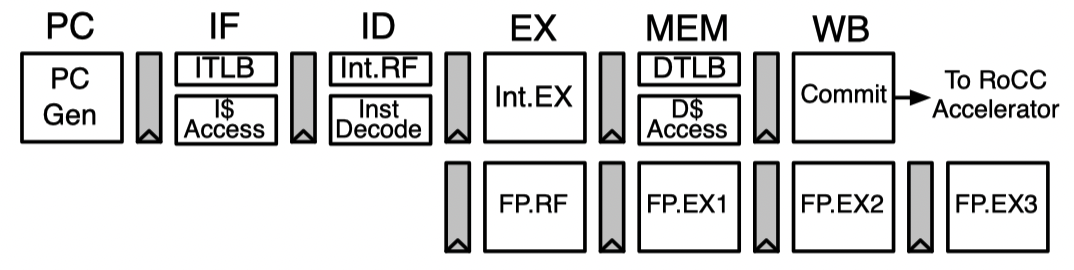
\includegraphics[width=0.95\textwidth]{Photos/Rocket_Pipeline.png}
	\caption{Rocket的流水线结构}
\end{figure}

Rocket面向的应用场景为低功耗优化下的高性能嵌入式设备,在同等TSMC 40nm工艺条件下,相比起对标的ARM Cortex-A5微处理器,Rocket具有相近的性能表现以及更小的面积以及更低的功耗:Dhrystone评分A5为1.57,Rocket为1.72(单位为:DMIPS/MHz)。面积上A5为0.53$mm^2$,Rocket为0.39$mm^2$。动态功耗上A5小于0.08mW/MHz,Rocket为0.034mW/MHz。

BOOM[5]是RISC-V基金会开发的另一个标准RISC-V微处理器实现。与Rocket不同,BOOM采用的是超标量乱序执行流水线实现,支持指令集为RV64G。与Rocket相同,BOOM也使用Chisel进行设计实现,因此在BOOM当中复用了大量Rocket中实现的模块生成器代码。BOOM很大程度上受到MIPS R10000[6]以及Alpha 21264[7]实现的启发,与这两种实现相同,SonicBOOM实现采用了显式寄存器重命名[8]的技术。BOOM的流水线结构如图1-2所示,BOOM采用了10级流水线结构,译码阶段采用4路译码,乱序执行算法在Tomasulo算法基础上加入重排序缓冲区技术改进,使指令最终提交时维持发射顺序,以达到维护精确中断的效果。

\begin{figure}[htbp]
	\centering
	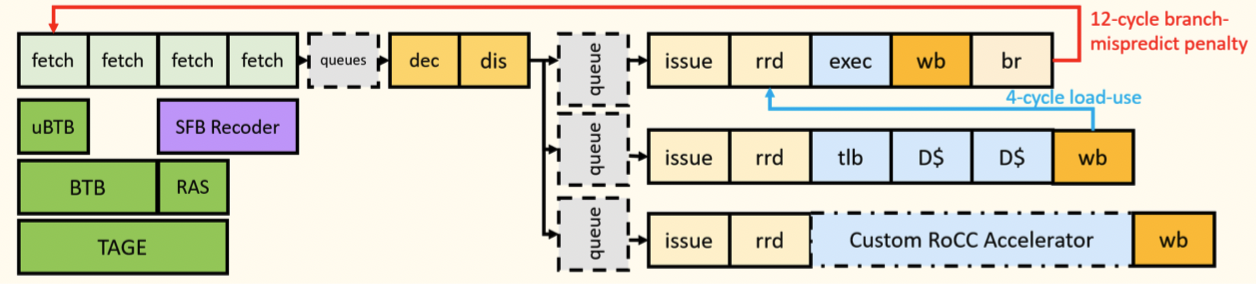
\includegraphics[width=0.95\textwidth]{Photos/BOOM_Pipeline.png}
	\caption{BOOM的流水线结构}
\end{figure}

BOOM面向的应用场景为兼具高性能以及高能效的消费类移动端/网络设备,在同等TSMC 40nm工艺条件下,相比起对标的ARM Cortex-A9微处理器,BOOM具有稍好的性能表现,同时具有更小的面积以及更低的功耗:CoreMark评分A9为3.59,BOOM为3.91(单位为CoreMarks/MHz)。面积上A9约为2.5$mm^2$,BOOM约为1.00$mm^2$。功耗上A9为0.5-1.9W,工作主频为0.8-2.0 GHz,BOOM为0.25W,工作主频为1 GHz。

Hummingbirdv2 E203[9]是国内芯来公司所研发的面向超低功耗及面积优化的嵌入式设备RISC-V微处理器,支持RV32IMAC以及RV32EMAC指令集,两级顺序执行流水线结构,且仅实现了机器级特权模式。E203的主要亮点在于其可配置的NICE(Nuclei Instruction Co-unit Extension)系统,可以允许用户自定义指令,在保持低功耗的前提下提升与外部领域专用加速器交互的性能。E203的SoC架构如图1-3所示。

\begin{figure}[htbp]
	\centering
	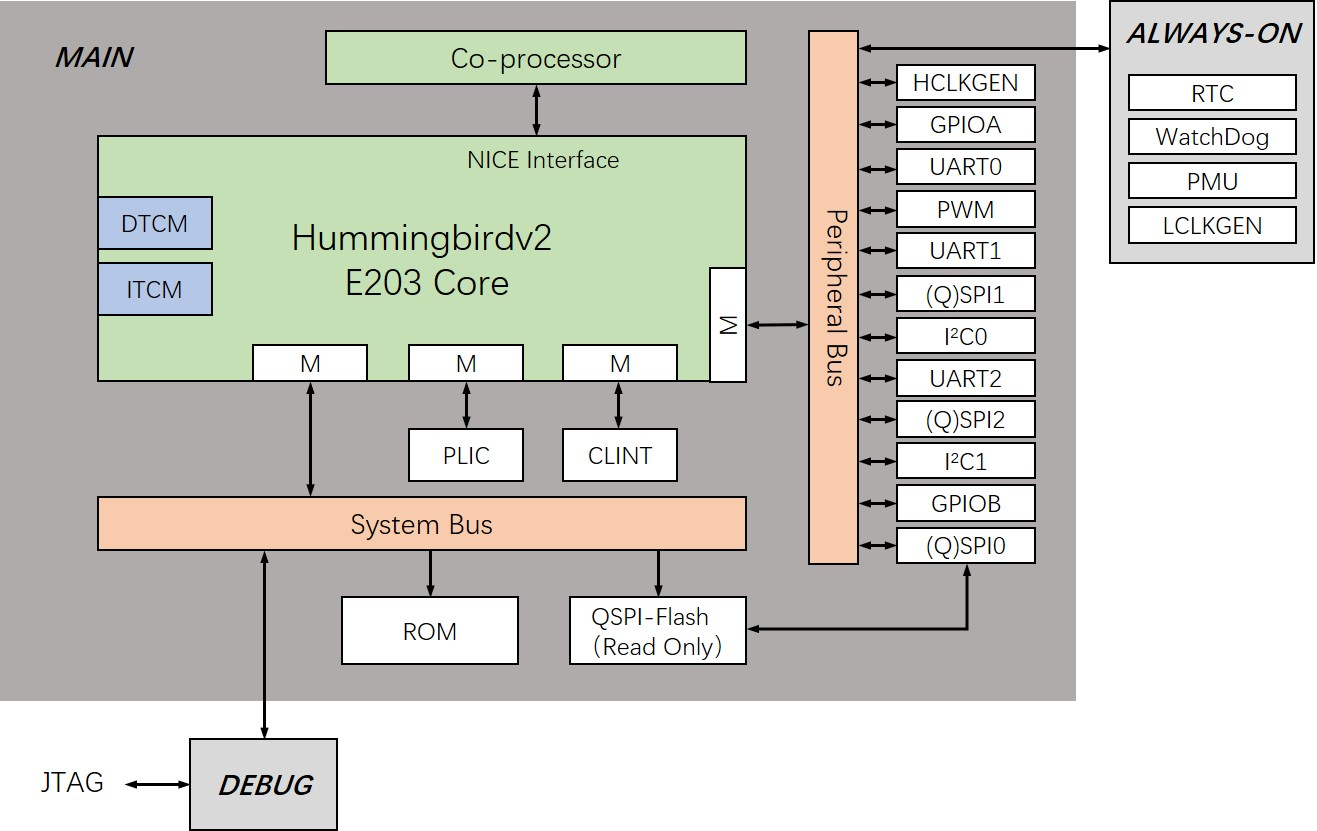
\includegraphics[width=0.95\textwidth]{Photos/hbirdv2_soc.jpeg}
	\caption{E203 SoC架构图}
\end{figure}

E203与其对标的ARM Cortex-M0/M0+相比,在维持相近的逻辑门数量前提下,能够达到更优的性能表现,且包含了多周期的硬件乘法与除法器:Dhrystone Cortex-M0与M0+的分数分别为0.84与0.93,而E203为1.23(单位:DMIPS/MHZ)。CoreMark Cortex-M0与M0+的分数分别为1.62与1.77,而E203为2.15(单位:CoreMarks/MHz)。三者逻辑门的数量都为12K。

PicoRV32[10]是由Clifford Wolf专为FPGA平台设计的面积深度优化的RISC-V微处理器实现。PicoRV32可以配置为支持RV32E,RV32I,RV32IC,RV32IM以及RV32IMC指令集的内核,同时带有一个可选的内置中断控制器。PicoRV32在Xilinx 7-Series FPGA开发板上仅占用750-2000 LUTs,且能够达到250-450MHz的工作频率。鉴于其优秀的性能与面积以及可选的协处理器接口,可以很容易的将一些针对FPGA的特定应用协处理器(音视频加速器、神经网络加速器)等移植到包含PicoRV32的FPGA系统上。

RI5CY[11]微处理器项目是瑞士苏黎世联邦理工大学(ETH Zürich)的综合系统实验室(IIS:Integrated Systems laboratory)和意大利博洛尼亚大学(University of Bologna)的高能效嵌入式研究组(EEES:Energy-efficient Embedded Systems)联合设计研发的PULP[12](Parallel Ultra-Low Power)项目中的其中一个子项目。PULP的目的是实现一个开放、可扩展的SoC,其包含的子项目如图1-4所示。其主要目的是解决IoT设备中日益增长的大量运算负载的场景。PULP支持多种处理器核架构,RI5CY是其中的一种处理器核实现。RI5CY是一款4级流水线的32位RISC-V微处理器,其包含了RV32IMC以及可选的“F”单精度浮点数扩展指令集实现。同时,为了提高DSP处理性能,RI5CY还包括自定义指令集如硬件循环(Hardware Loop)、乘累加(MAC)指令以及向量操作指令等。目前RI5CY项目已经迭代为CV32E40P[13]微处理器项目,在RI5CY的项目基础上添加了对标准RISC-V核内本地中断控制器以及高级调试模式的支持。

\begin{figure}[htbp]
	\centering
	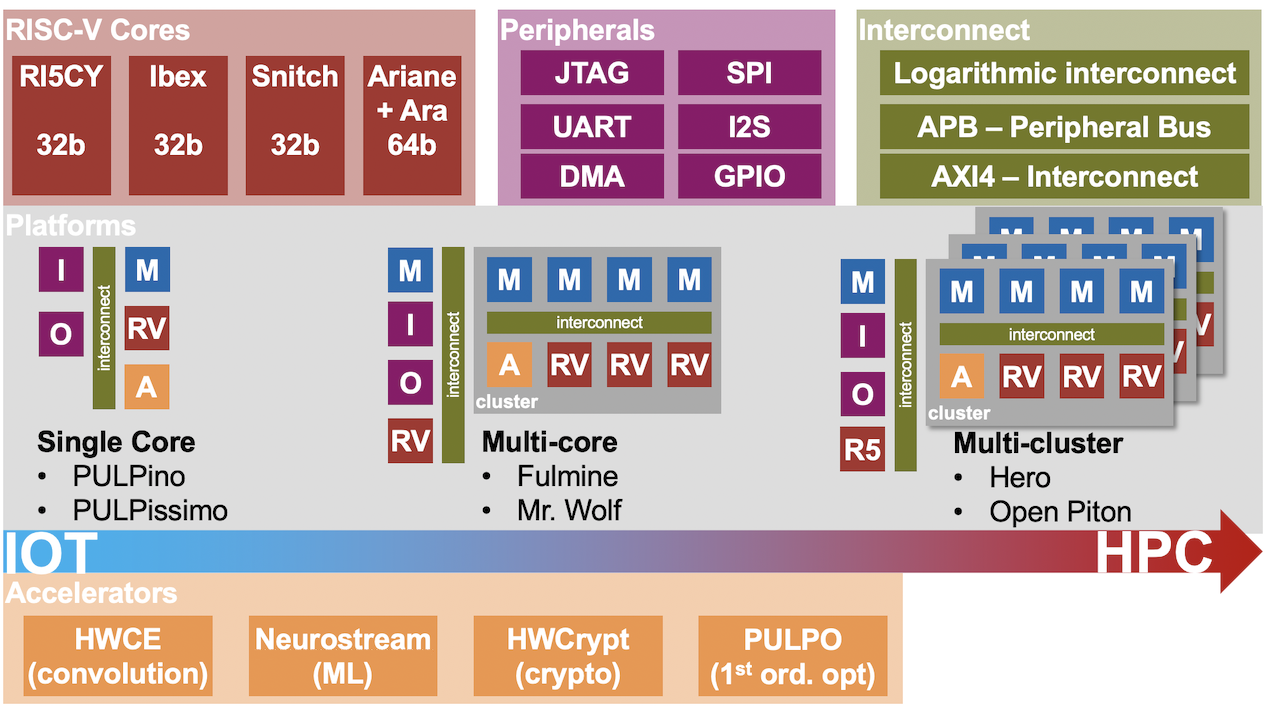
\includegraphics[width=0.95\textwidth]{Photos/pulp_family.png}
	\caption{PULP项目平台概览}
\end{figure}

RI5CY在性能上与其对标的Cortex-M4微处理器基本持平,在面积以及动态功耗上都要优于Cortex-M4:CoreMark Cortex-M4的分数为3.40,而RI5CY为3.19(单位:CoreMarks/MHz)。在65ns的工艺下,Cortex-M4的动态功耗以及面积分别为23.2µW/MHz、0.062$mm^2$,而RI5CY则分别为17.5µW/MHz、0.050$mm^2$。

香山[14, 15]是由中国科学院计算技术研究所在2021年发布的一款开源高性能RISC-V处理器,使用了包括Chisel、Verilator、GTKwave 等在内的大量开源工具,实现了差分验证、仿真快照、RISC-V 检查点等处理器开发的基础工具,建立起了一套包含设计、实现、验证等在内的基于全开源工具的处理器敏捷开发流程。香山处理器实现了RV64GC指令集,采用乱序六发射结构设计,前端包括取指单元、分支预测单元、指令缓冲等单元,顺序取指。后端包括译码、重命名、重定序缓冲、保留站、整型/浮点寄存器堆、整型/浮点运算单元。香山处理器使用了分支预测器向前覆盖的机制来实现分支预测策略,主要目的在于使用使用容量大、预测算法更复杂、得到指令信息越多的预测器来保证更高的预测准确率,但缺点在于预测器得出结果的延迟比较高,因此香山还使用了一些小型的预测器进行先行预测。香山处理器的架构如图1-5所示。

\begin{figure}[htbp]
	\centering
	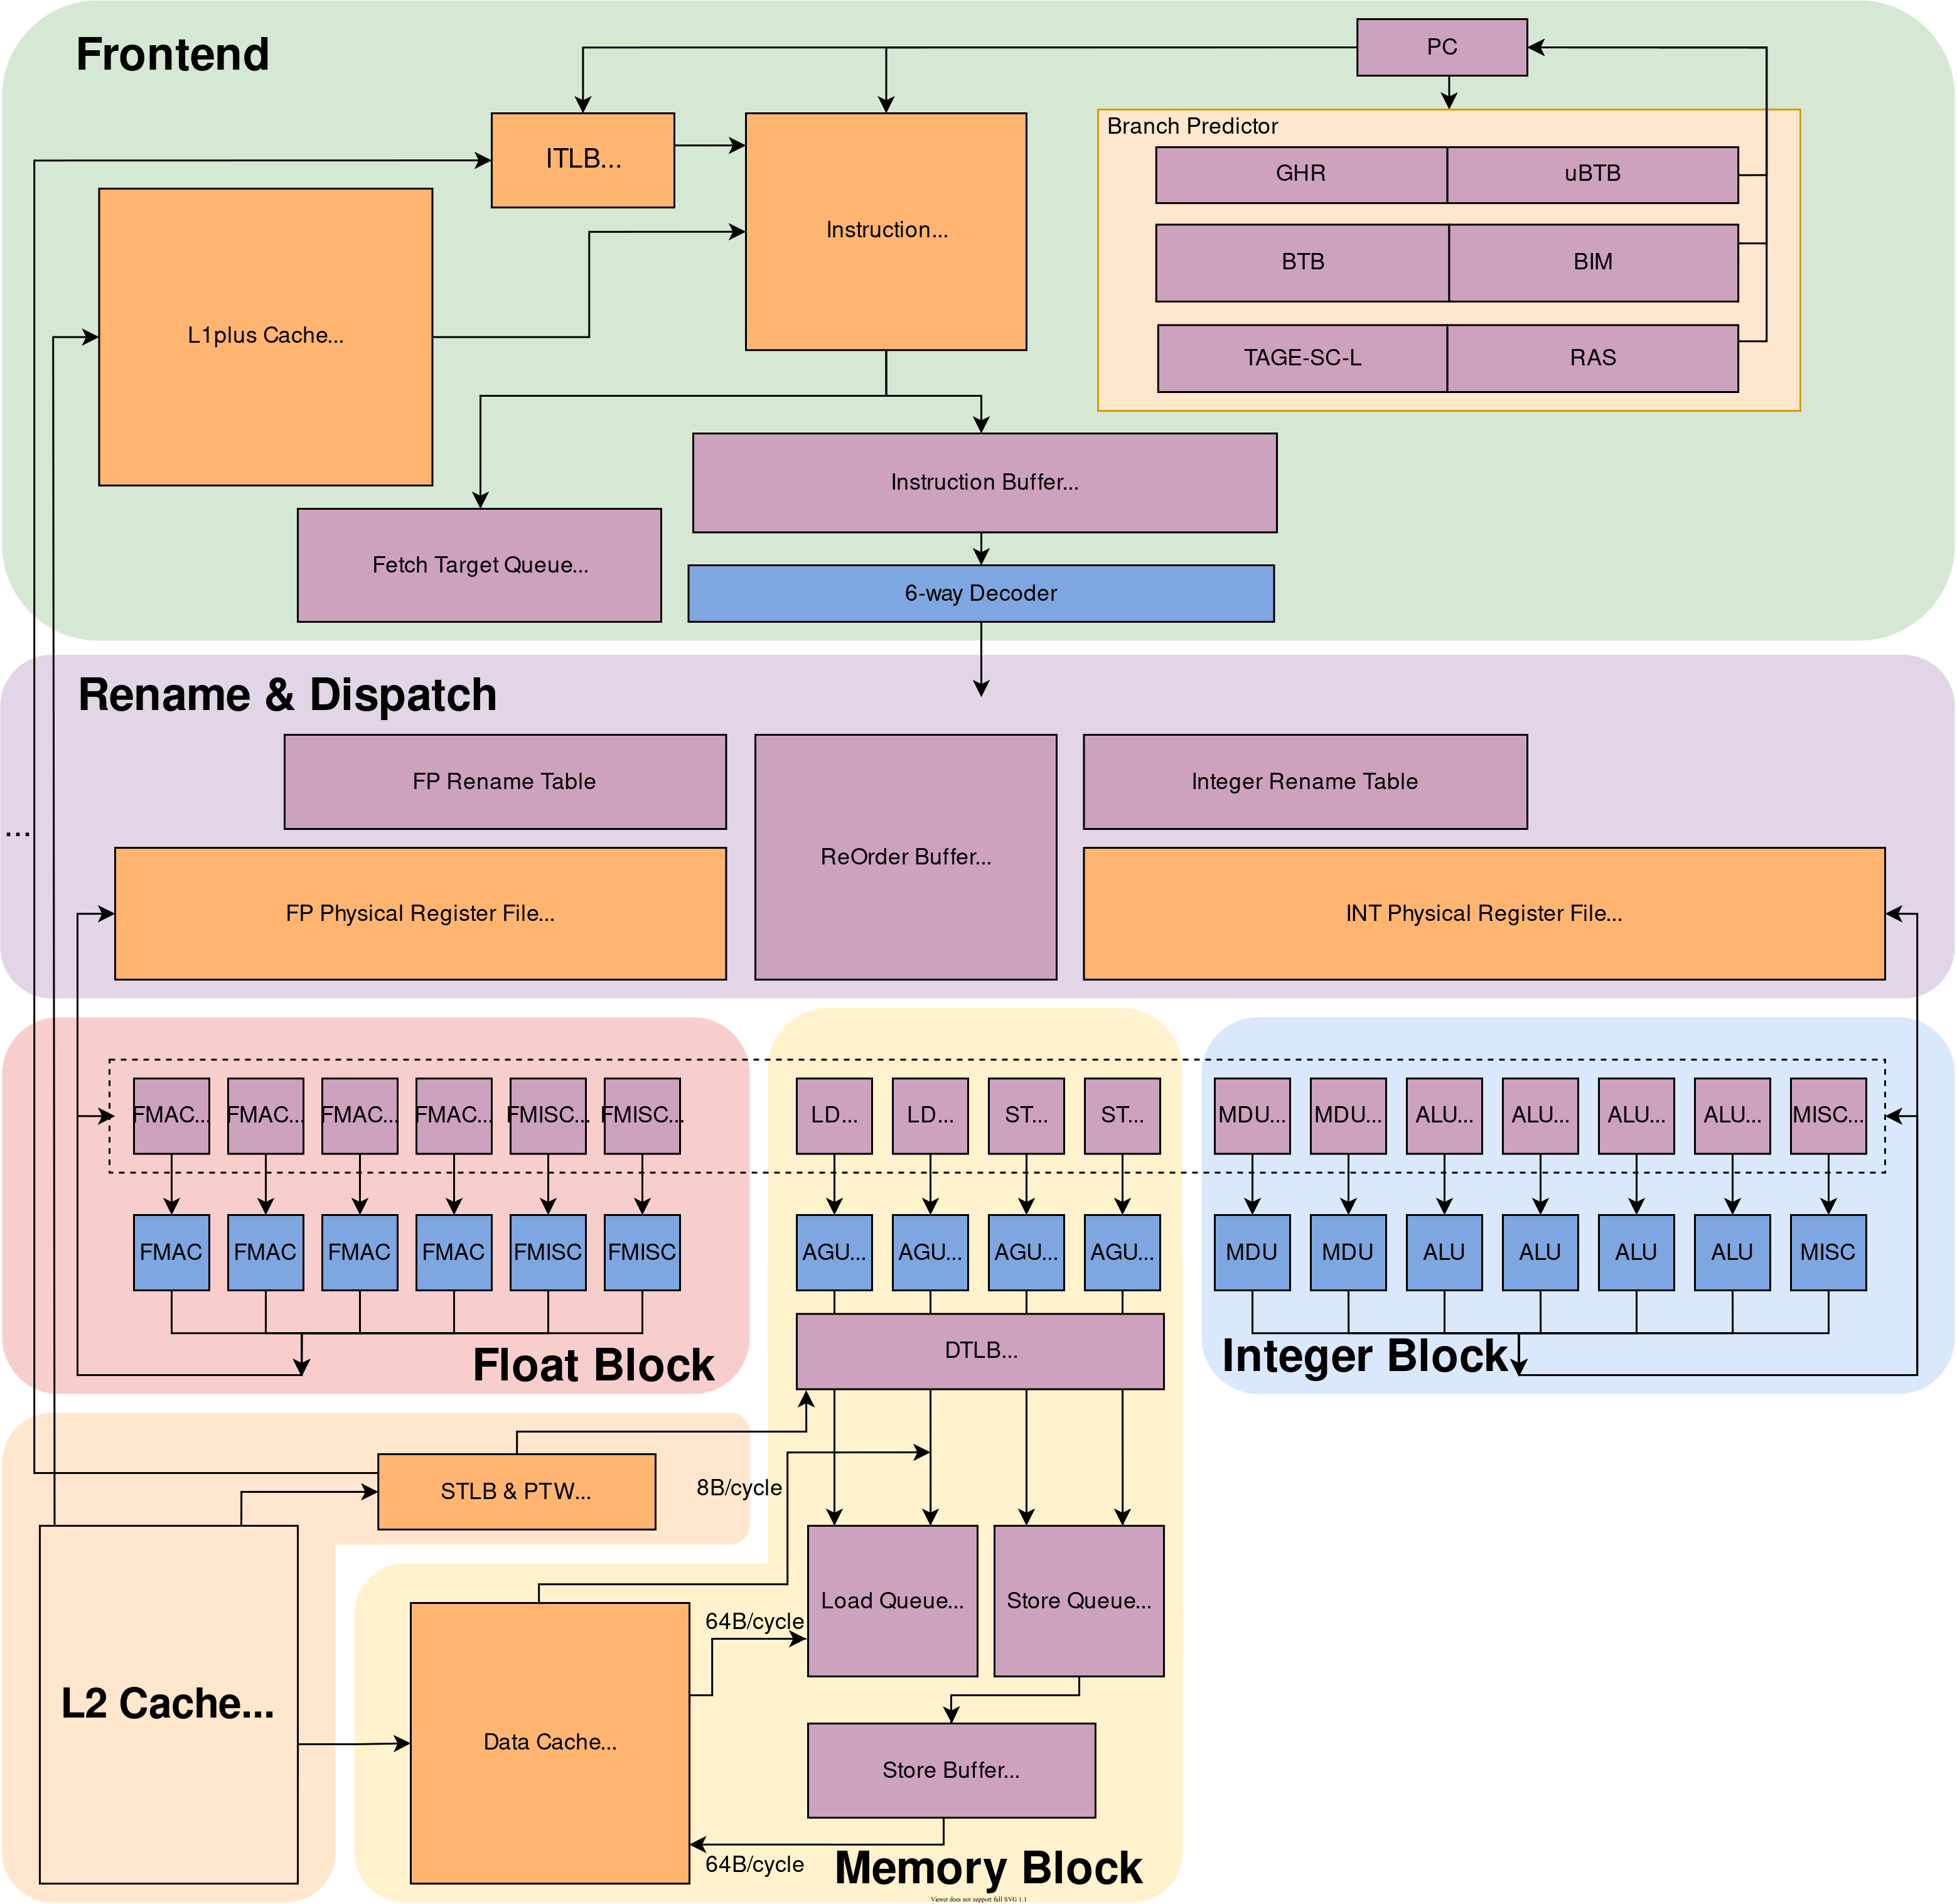
\includegraphics[width=0.95\textwidth]{Photos/xs-arch-simple.png}
	\caption{香山处理器架构图}
\end{figure}

香山处理器具有不俗的性能表现,香山的第一版架构“雁栖湖”在28nm工艺的频率上能够达到1.3GHz的频率。而目前正在开发的第二版架构“南湖”则在14nm工艺上能够达到2GHz的频率。并且,香山处理器目前已经在FPGA部署上启动了Linux/Debian操作系统,成为第一个国内完全开源的支持UNIX系统的微处理器。

\section{硬件设计方法学概论}
\subsection{研究背景}

囿于丹纳德缩放定律以及摩尔定律的终结,现今计算机体系结构面临着数个显著的挑战。丹纳德缩放定律的失效使得功耗变为现今集成电路设计的首要关键因素,而摩尔定律的终结则减缓了对晶体管技术的进步。因此,计算机架构师必须要寻找其他的途径来提高计算机系统的整体性能,这其中的重要策略之一则是使用领域特定架构(Domain Specific Architecture,DSA),也就是所谓的加速器来构成异构的计算机系统。然而,传统的硬件开发方法论缺乏在进行异构系统的设计时,缺乏相应的生产力以及效率。在过去的数十年中,瀑布模型一直是硬件开发流程所使用的设计模式,如图1-6所示。在瀑布模型的设计模式当中,开发者必须在当前阶段全部完成后才能够进入下一个阶段。举例来说,开发者只有对当前芯片所有功能的RTL设计完成后,才能够进入前端验证的阶段。如果在任意一个阶段中发现问题,则需要放弃该阶段中所有已经完成的工作而回退到上一阶段重新进行设计,且越进行到后续的阶段,解决问题的成本将会指数型的上升。

\begin{figure}[htbp]
	\centering
	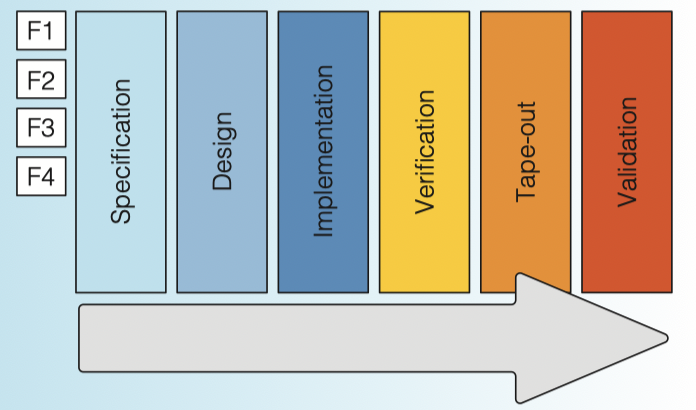
\includegraphics[width=0.95\textwidth]{Photos/waterfall.png}
	\caption{硬件开发流程中简易的瀑布模型示意,F1~F4表示了该设计的功能单元。从左到右的阶段分别为设计需求分析、架构设计、(RTL)实现、验证、流片、样片功能测试。可以发现瀑布模型中设计所有的功能单元完成当前阶段的开发后才能进入下一个阶段。实际开发流程中每个阶段都包含了相当多的具体步骤。}
\end{figure}

为了解决这个问题,伯克利大学的计算机体系结构研究团队(BAR)提出了硬件敏捷设计的方法学[16]。硬件敏捷设计的主要思想是通过快速迭代开发不完全功能的原型系统来达到敏捷设计的效果。举例来说,对于一个基于RV32G指令集微处理器的实现,硬件敏捷设计方法通过快速开发一个仅支持RV32I的芯片原型并进行流片,以获得在当前工艺下原型设计的具体参数,并以此为基础修正原先的设计。在此基础上,再添加乘除法、浮点等功能单元,并最终迭代得到成品。在硬件敏捷开发的设计模式下,当功能A进入下一阶段时,负责当前阶段的团队可以立即着手对功能B的开发。硬件敏捷开发的设计模式如图1-7所示。

\begin{figure}[htbp]
	\centering
	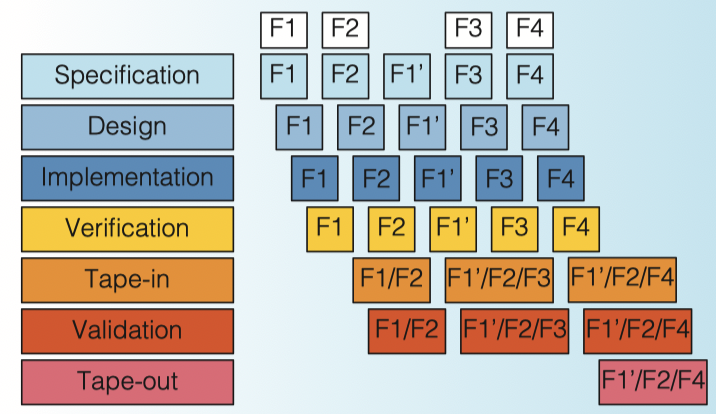
\includegraphics[width=0.95\textwidth]{Photos/agile_hardware_dev.png}
	\caption{硬件敏捷开发设计模式示意图}
\end{figure}

为了在硬件开发中引入敏捷设计模式,还需要对硬件设计工具以及框架进行改进,传统的Verilog/SystemVerilog语言无法匹配敏捷设计的需求,因此,近几年来大量基于高层次语言的硬件生成框架(Hardware Generation Frameworks,HGFs)应运而生。除了通过引入敏捷设计模式来提高硬件开发的效率,还有一种可以显著加速异构计算体系设计的方法:通过高层次综合(High-Level Synthesis,HLS)[17]的方法设计加速器。HLS允许用户将所需要实现的加速器算法以特定的C/C++语言描述出来,并通过专用的编译器生成优化过的Verilog代码。然而HLS对于架构师来说具有相当曲折的设计曲线,且目前HLS的设计优化仍然主要依赖于经验。因此,本文将重点主要放在基于高层次语言的硬件生成框架/语言当中,下一节将会介绍目前国内外对基于高层次语言的敏捷设计驱动的硬件生成框架/语言进行介绍。

\subsection{国内外研究现状}

早期对于硬件生成框架的研究项目有Verischemelog[18],它将Verilog语言混入Scheme[19]语言当中来描述硬件结构。早期的硬件生成框架项目还有Genesis2[20],它与Verischemelog的思路类似,但Genesis2是将Verilog语言混入到Perl语言当中。早期的硬件生成框架的设计都比较粗糙,一般仅使用字符串处理的方法来生成设计的Verilog代码,整体的编译过程都是静态的。因此,这些架构都缺乏可扩展性以及灵活性。

Chisel[21]是现代硬件生成框架的先驱,其作为RISC-V的衍生项目而诞生。Chisel并非简单的使用字符串处理的方式来将Verilog语言混入到某种高级语言当中,而是基于Scala[22]开发了一个完整的硬件开发库,其中包含了小到描述线网、寄存器、存储器、逻辑门的原语,大到算术逻辑单元、控制器、DSP的生成器。同时,Chisel还包含了一个介于Chisel以及Verilog之间的中间语言层FIRRTL[23, 24],它本质上是一个高度抽象化的RTL级语言。由于Chisel本质上属于使用Scala开发的第三方库,因此使用Chisel进行RTL级的硬件描述,并且支持Scala所有的语言特性,包括参数化、面向对象编程、函数式编程等等,这些特性在硬件敏捷开发模式当中将起到关键的作用。截至目前,已经有多个使用Chisel开发的微处理器、SoC以及加速器项目,如上面提到的Rocket、BOOM以及Raven-3[25]、FireSim[26]、ChipYard[27]等等。然而,Chisel在验证方面并没有给出比较完善的解决方案。目前Chisel仅支持使用基于Chiseltest[28]的单元测试验证方法,并不支持对于基于大规模的功能测试、系统测试的UVM验证方法学。Chisel整体的框架如图1-8所示。

\begin{figure}[htbp]
	\centering
	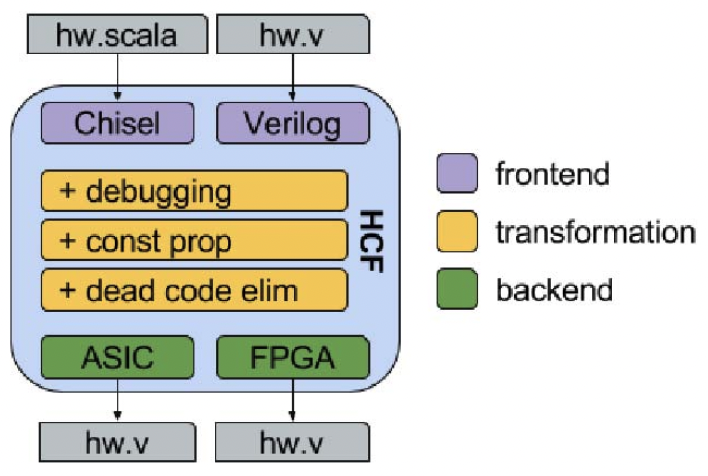
\includegraphics[width=0.95\textwidth]{Photos/chisel.png}
	\caption{Chisel整体框架图}
\end{figure}

与Chisel类似,使用Scala作为高层语言宿主的硬件生成框架还有SpinalHDL[29]。SpinalHDL最初是为了解决Chisel所缺乏的多时钟域功能所诞生的衍生性项目。与Chisel不同,SpinalHDL在设计之初采用更偏向于实际工程开发的风格,支持常见的EDA工具链。SpinalHDL不具有FIRRTL中间层,而是从Scala直接编译为对应的Verilog代码,且编译过程中不存在黑盒机制。并且,SpinalHDL不会带来额外的面积或者性能上的开销。因此,SpinalHDL相对于Chisel要更受工业界的欢迎,而Chisel则普遍受众于学术界研究。

相比较于近年来才开始流行基于Scala的硬件生成框架,基于Python的HGF设计在世纪初就开始有项目进行尝试。PyHDL[30]是最初较为流行的基于Python的脚本式硬件描述语言,它使用PamDC以及PAM-Blox两个C++硬件设计库扩展Python语言,其中,PamDC提供了硬件描述语言所需要的原语如寄存器以及线网,而PAM-Blox则是使用PamDC原语构造的工具集,包含了参数化以及面向对象的硬件模块。MyHDL[31]是一个免费开源的用于硬件描述以及验证的Python库。MyHDL将Python代码编译为Verilog或者VHDL并提供基于Python的设计代码与主流EDA工具交互的方法。MyHDL包含一个运行在Python解释器顶层的仿真器,并使用PLI(Procedural Language Interface)来与仿真器进行交互。然而,基于Python的仿真器在性能上存在劣势,并且MyHDL并不支持基于UVM的验证方法。Stratus[32]是一个基于Python的超大规模集成电路(Very Large Scale Integration,VLSI)描述语言,Stratus通过一系列的方法以及函数对Python进行扩展,来生成VLSI设计的线网(Netlist)模型。PHDL[33]同样使用Python作为硬件描述的语言,其主要亮点在于包含一个内置的模块库用于微处理器设计。然而PHDL不包含任何验证的工具或方法,仅提供了针对微处理器开发的设计模式。Migen[34]与Stratus类似,也是基于Python的VLSI设计工具,Migen基于硬件描述语言FHDL,它包含了一个形式化描述的系统来描述电路中的组合电路信号或时序电路状态。同样,Migen仅仅专注于对系统的描述,而缺乏对所设计电路的验证方法。PyRTL[35]是一个新兴的基于Python的开源硬件设计语言,与Chisel类似,它主要的设计目标在于快速的硬件原型构建。PyRTL与PyHCL一样,都是为了达到对硬件描述的简洁化。然而,PyRTL依然缺乏对设计的验证方法或工具,仅提供了一个效率低下的内置仿真器。PyMTL[36]及其后代版本Mamba[37]是一个基于Python的多层次的硬件建模工具, 它的主要特点在于使用的是在三种层次:功能级(Functional Level)

时钟周期级(Cycle Level)以及RTL级上的建模。PyMTL提供了基于PyPy JIT(即时编译)解释器的仿真器,然而其效率相比业界基于C/C++的开源仿真器Verilator仍然存在不小的差距。表1-1对上述提到的硬件生成框架与PyHCL进行对比。

\begin{table}
	\caption{PyHCL以及其他硬件生成框架的对比}
	\centering
	\small 
	\begin{tabular}{cccccc}
		\hline 
		框架 & 宿主语言                & 敏捷硬件设计支持 & 宿主语言模式 &     内置仿真器 &  UVM支持            \tabularnewline
		\hline 
		PyHCL   & Python		     & 是   & 原语构造型 & 否 & 是 \tabularnewline
		Chisel    & Scala		         & 是   & 原语构造型 & 是 & 否 \tabularnewline
		PyRTL   & Python		     & 是   & 描述型 & 是 & 否 \tabularnewline
		MyHDL   & Python		     & 否   & 描述型 & 是 & 否 \tabularnewline
		PyHDL   & Python		     & 否   & 描述型 & 否 & 否 \tabularnewline
		PHDL   & Python		     & 否   & 描述型 & 否& 否 \tabularnewline
		PyMTL/Mamba   & Python		     & 是   & 多层次建模 & 是 & 否 \tabularnewline
		\hline 
	\end{tabular}
\end{table}

\section{本文的创新点以及难点概述}

通过1.1节对国内外基于RISC-V的开源微处理器实现以及1.2节对国内外开源硬件生成框架的概述,可以看出:

\begin{enumerate}
	\item 在开源微处理器设计方面,目前开源的微处理器架构中,还不具备有使用P扩展指令集来实现的基于RISC-V的DSP微处理器。RI5CY虽然是一款专用于DSP的微处理器架构,但由于其使用了大量的非标准化的指令,导致其整个上层的软件生态链都需要靠自定义的编译器实现,也缺乏足够的扩展性和稳定性。同时,基于P指令集实现的RISC-V开源微处理器现在还没有先例,目前大多数面向数字信号处理的RISC-V微处理器都是采用V指令集或者裁剪V指令集的方式来实现,这种方式对于芯片整体面积以及编译器实现都会带来不必要的麻烦。
	\item 在开源硬件生成框架方面,某些的HGF仅支持设计功能,某些HGF包含有内置的仿真器,但是效率比较低下,且目前还没有HGF包含有内置的UVM验证方案。
\end{enumerate}

针对以上的问题,本文所实现的基于P扩展指令的面向DSP的RISC-V嵌入式微处理器以及基于Python的开源硬件生成框架PyHCL具有以下的创新点:

\begin{enumerate}
	\item 本文所实现的RISC-V微处理器是目前唯一的开源实现P指令集的DSP微处理器,P指令集采用SIMD指令方式来实现DSP运算库中所需要的算法,其实现虽然比V扩展指令集缺乏一定的灵活性,但是在逻辑复杂度方面要简单许多,最终实现的芯片在逻辑门数、面积、功耗方面要比V扩展指令集占优。
	\item 本文所实现的RISC-V微处理器使用并行数据通路的方式来实现P指令集,在性能上虽然要略逊于基于RoCC的协处理器实现方式,但能够得到更小的芯片面积,更适合应用在嵌入式场景当中。
	\item PyHCL同时包含了设计以及验证工具链,是首个基于Python的全栈硬件生成框架。PyHCL允许集成电路设计以及验证的流程都在同一个框架内完成,而不需要分离为多个不同的工具链以及框架,加速硬件开发的迭代速度。
	\item PyHCL还提供了基于UVM的验证方法学的解决方案,是首个支持UVM验证方法学的开源硬件生成框架,且PyHCL还包含了灰盒测试及多级测试的验证策略,覆盖了从单元测试到集成测试的验证粒度。
\end{enumerate}

本文的微处理器实现以及开源硬件生成框架PyHCL的实现存在以下的难点:

\begin{enumerate}
	\item 目前业界缺乏基于P指令集的开源微处理器实现,且P指令集标准仍然处于草案状态,对于微处理器的设计、验证以及性能测试会带来一定的难度。
	\item 使用多数据通路的并行实现方式,对微处理器的控制逻辑实现会带来比较大的负担,这是因为SIMD指令大多数需要多个周期来实现,则微处理器需要处理好处理器停顿以及数据冒险、控制冒险等问题。
	\item 集成多种验证测试方法在同一个Python框架中需要保证对用户接口的统一性,否则会破坏PyHCL设计的初衷,即在同一框架模型中集设计与验证为一体。
\end{enumerate}

\section{本文的章节安排}

本文分为五个章节,其余章节的内容作以下的组织安排:

第二章:基于Python的硬件开发框架PyHCL。本章对PyHCL的架构进行概述,包括PyHCL原语、接口、中间表示层IR等。最后介绍了结合FIRRTL作为后端生成语言的数种优势。

第三章:面向DSP的嵌入式微处理器设计与实现。本章对实现了RISC-V RV32GCP指令集的微处理器进行介绍,包括对微处理器的基本流水线设计、特权级设计、多数据通道设计等等进行介绍。最后对包含了该微处理器的SoC平台进行介绍。

第四章:PyHCL验证方法概述。本章对PyHCL支持的多种验证方法进行概述,包括基本单元测试使用的PyHCL-Tester、基于UVM的大规模集成测试框架PyUVM、针对RISC-V微处理器的差分测试框架等的介绍。

第五章:总结与展望。
%第一章
	\chapter{基于Python的硬件开发框架PyHCL}

本章将会介绍用于开发本文所实现的RISC-V微处理器以及SoC平台所使用的基于Python的硬件开发框架PyHCL的技术细节,包括对PyHCL的接口、中间语法树IR、生成器(emitter)以及PyHCL后端生成的FIRRTL语言。在本章的最后会给出PyHCL设计中的创新点以及其如何解决现有硬件开发框架与工具链中固有的问题。

PyHCL的整体设计工具链可以总结如下:开发者使用PyHCL的用户接口在RTL级上对电路逻辑进行描述。为了复用FIRRTL语言作为高层次抽象RTL描述的优势,PyHCL的后端目标生成语言设定为FIRRTL。为了生成FIRRTL代码,PyHCL会根据顶层基于PyHCL接口的电路描述构造中间语法树IR。之后,PyHCL生成器基于语法树生成等效的FIRRTL代码,并将其作为FIRRTL编译器的输入,并将其转化为类网表结构的LoFIRRTL模型,开发者可以在FIRRTL级别上对网表结构进行调整。最后,LoFIRRTL模型转化为可综合的Verilog代码,并可以作为EDA工具的输入进入后端的设计流程。PyHCL设计流程如图2-1所示。

\begin{figure}[htbp]
	\centering
	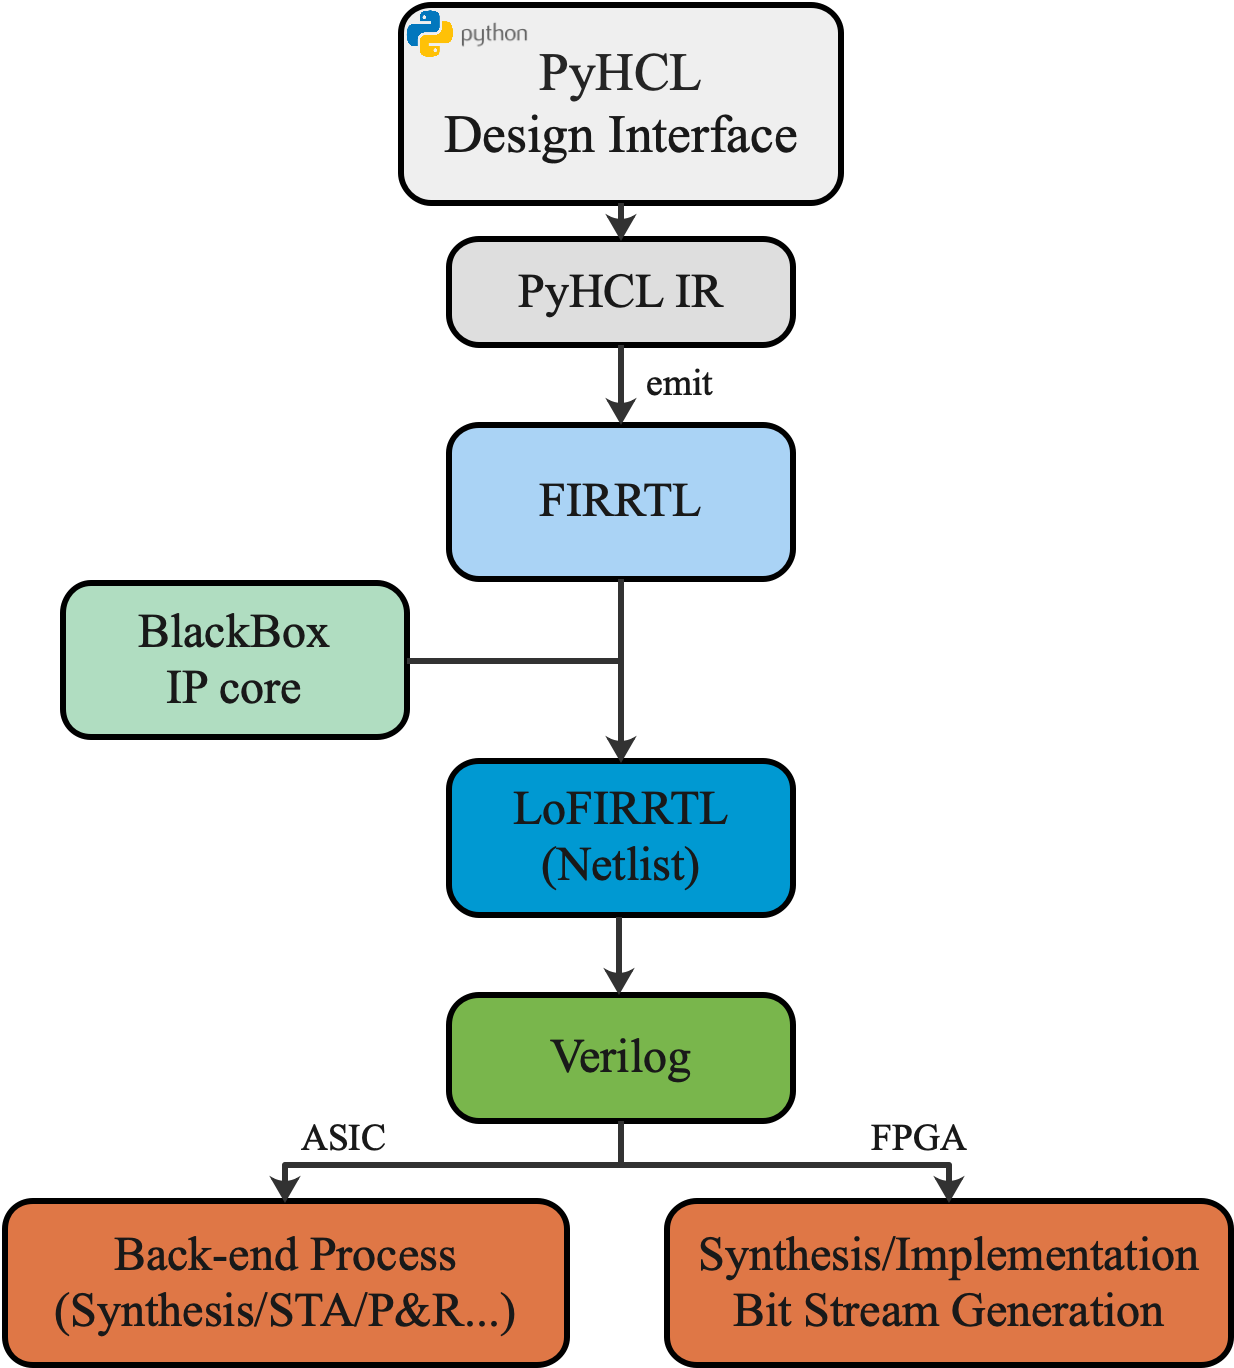
\includegraphics[width=0.95\textwidth]{Photos/PyHCL-Overview.png}
	\caption{PyHCL设计流程}
\end{figure}

\section{PyHCL接口}

PyHCL的设计哲学在于简洁高效的构造(Constructing)电路,而不是单纯的描述(Description)。因此,PyHCL提供了标准的PyHCL数据类型、运算符以及电路元素在RTL级别上构造电路。到目前为止,PyHCL支持三种基本的数据类型:无符号整型(U)、有符号整型(S)以及布尔类型(Bool),其中布尔类型是特殊的无符号类型,在实现时约束为1位的无符号类型来看待。除此之外,PyHCL还支持两种复杂数据类型,分别为向量类型(Vec)以及捆绑类型(Bundle)。向量类型支持对一组相同大小与类型的基本类型数据进行操纵,主要在处理SIMD运算时使用,可以类比为数组。捆绑类型则支持对一组不同大小与类型的基本类型数据进行操作,主要在总线协议接口时使用,可以类比为集合。除此之外,PyHCL还支持隐式的内置时钟类型Clock。通过自定义布尔类型的输入端口,PyHCL支持模块内的多时钟域设计,可以很好的支持异步FIFO[38]等跨时钟域结构的设计。模块内置的隐式或者用户自定义的显式时钟端口可以被模块内部以及外部其他模块引用。

PyHCL运算符通过重载Python内置的运算符来实现。其中最重要的运算符为连接运算符“<<=“,它的作用是驱动右表达式的信号加载到左表达式当中,这涉及到了两个主要的问题:

\begin{enumerate}
	\item 如何匹配Verilog在RTL级描述中的阻塞赋值以及非阻塞赋值。在PyHCL的电路构造过程中,对时序信息是隐含的,对赋值方式的处理在生成Verilog时进行。对于被驱动的电路实体元素,如果是线网类型,则统一使用阻塞赋值。如果是寄存器类型,则统一使用非阻塞赋值。换句话说,开发者在构造电路时不需要考虑赋值类型问题,而只需要关注信号的流动。
	\item 驱动信号与被驱动的电路实体之间的方向关系。PyHCL在构造中间语法树的过程中会对信号的流动方向进行检查,如果发现违例(如模块内部信号连接运算符的左表达式是输入端口),则会抛出异常。
\end{enumerate}

PyHCL接口常用的数据类型及运算符如表2-1所示。

\begin{table}
	\caption{PyHCL常用数据类型及运算符列表}
	\centering
	\small 
	\begin{tabular}{cc}
		\hline 
		PyHCL数据类型 & 用法 \tabularnewline
		\hline 
		\texttt{U} & 无符号整型  \tabularnewline
		\texttt{S} & 有符号整型  \tabularnewline
		\texttt{Bool} & 布尔类型,实现为1位无符号整型  \tabularnewline
		\texttt{Clock} & 隐式内置数据类型,用于表示模块时钟  \tabularnewline
		\texttt{Vec} & 创建一个可索引的包含相同位宽的数据类型的向量结构 \tabularnewline
		\texttt{Bundle}  & 创建一个包含不同位宽的数据类型的集合 \tabularnewline
		\hline
		PyHCL运算符 & 用法 \tabularnewline
		\texttt{<<=} & 连接运算符 \tabularnewline
		\texttt{==}, \texttt{!=} & 逻辑相等,逻辑不等 \tabularnewline
		\texttt{\&}, \texttt{|}, \texttt{\^}, \texttt{\~} & 按位与,按位或,按位异或,按位取反 \tabularnewline
		\texttt{+}, \texttt{-}, \texttt{*}, \texttt{/}, \texttt{\%} & 算术运算符 \tabularnewline
		\texttt{>}, \texttt{>=}, \texttt{<}, \texttt{<=} & 算术比较运算符 \tabularnewline
		\texttt{<<}& 逻辑左移 \tabularnewline
		\texttt{>>} & 逻辑(U)/算术(S)右移,取决于操作数的类型  \tabularnewline
		\texttt{[]} & 位提取运算符,如[5:1]为提取信号第1位到第5位的数据 \tabularnewline
		\hline 
	\end{tabular}
\end{table}

PyHCL接口中提供的电路实体元素是实际电路构造中的功能单元,包括寄存器、线网以及存储单元,它们的PyHCL表示分别为Reg,Wire,以及Mem。所有的PyHCL电路实体元素都预定义在库中,开发者只需要实例化这些电路实体元素就能在设计中使用。PyHCL的电路设计是基于模块化的设计,定义模块的方式通过继承Module基类来实现。为了降低设计者的负担,PyHCL对模块间以及顶层模块与子模块之间的连接提供了自动连接的功能。对于同一层次的两个模块之间的连接,当指定PyHCL进行自动模块连接时,PyHCL在生成语法树时会搜索两个同级模块之间方向相反的IO端口,如果这些端口之间有同样的数据类型、位宽以及名字,或者属于同一个Bundle实体,则PyHCL会将这些IO端口自动连接起来。对于父子节点关系的模块,则需要判断这些端口之间方向相同的IO端口。除此之外,PyHCL的IO端口可以是多级的,在设计总线协议相关的端口时,可以将协议定义的端口作为一个基础的Bundle实体,所有实现了该总线协议接口的模块IO端口都可以包含该Bundle实体。这种多级继承或包含的设计模式与传统的Verilog线性的IO端口声明要更具有鲁棒性。

PyHCL与传统的硬件描述语言的区别在于,PyHCL兼容所有Python的语言特性。所有的PyHCL电路实体元素都可以作为标准的Python内置变量或者实体被解释器所识别。除此之外,PyHCL接口支持多种高级语言特有的设计模式,对于电路设计来说,最具有代表性的两种特性分别是函数式编程以及参数化生成器。

与Verilog中所使用的以变量为中心的设计模式不同,函数式编程以函数为中心,而不是变量,一个函数可以接受其他函数作为参数,也可以返回一个函数对象。这种设计模式更为抽象,且可以将算法以更接近于数学语言的形式表示出来。因此,基于函数式编程的电路设计广泛应用于数字信号处理模块以及外部领域专用的协处理器当中[39]。以一个有限冲激响应(Finite Impulse Response,FIR)滤波器为例子:

\begin{equation}
	y[n]=\sum_{i=0}^N b_i \cdot x[n-i]
\end{equation}

其中N是滤波器的阶数,$b_i$是N阶滤波器在第i时刻($0 \leq i \leq N$)的脉冲响应,$x[n]$是输入信号,$y[n]$是输出信号。在不考虑面积以及性能约束的情况下,这里给出一个对上述滤波器电路实现的PyHCL代码作为例子:

\begin{lstlisting}
	def firFilter(length: int):
		consts = [U(1) for _ in range(length)]
		class FirFilter(Module):
			io = IO(i=Input(U.w(8)), o=Output(U.w(8)))
			taps = [io.i] + [RegInit(U.w(8)(0)) for _ in range(length-1)]
			for a, b in zip(taps, taps[1:]):
				b <<= a
			m = map(lambda x: x[0] * x[1], zip(taps, consts))
			io.o <<= reduce(lambda x, y: x + y, m)
		return FirFilter()
\end{lstlisting}

PyHCL鼓励开发者在电路描述当中使用函数式编程。一个应用函数式编程的典型代码包括两个主要的要素:函数聚合编程以及匿名函数。函数聚合编程表示函数可以作为另一个函数的输入以参数的形式进行传递,抑或是函数作为返回值返回。匿名函数则是临时创建的没有指定名称的函数,匿名函数常常作为函数参数来使用。在上述例子中,PyHCL使用了Python原生的高阶函数来满足上述的两个要素。首先,例子中使用了Python内置的map,zip以及reduce高阶函数来描述乘后加(MAC)运算。两个不同的匿名函数lambda则作为map以及reduce的函数参数来指导对输入信号以及脉冲响应系数的MAC运算。使用函数式编程描述的FIR滤波器更接近于数学语言,将基于Verilog描述中过于繁杂的时序信息隐藏起来,达到快速构建DSP或加速器模块的效果,使构建异构系统变得更有效率。

上述的例子当中除了将函数式编程应用到FIR滤波器的设计当中,还使用了参数化生成器的形式来构造FIR滤波器。可以发现,滤波器的阶数作为函数参数供调用者使用,该函数可以作为一个基础的滤波器生成模版,在其他模块当中进行复用。PyHCL中的参数化生成器中的参数并非是简单的字符串替换,在PyHCL语法树构建以及FIRRTL代码生成过程中参数也作为语法树的一部分,在转换为FIRRTL过程中进行相应的逻辑检查。

总的来说,PyHCL中大范围的函数式编程以及参数化生成器的使用显著的降低了电路设计的迭代周期,以此允许设计者在硬件敏捷设计模式当中应用。

\section{PyHCL IR}

PyHCL IR是介于PyHCL接口以及后端目标FIRRTL语言之间的中间语法树,它由多级的PyHCL IR节点构成。使用PyHCL构造的电路都对应一棵PyHCL语法树。为PyHCL设计介于前后端之间IR语法树的原因在于:

\begin{enumerate}
	\item 在PyHCL前端接口以及后端目标FIRRTL语言之间提供中间语法树可以显著降低PyHCL接口发生更改的风险。在未来,在需要改变接口设计的场合当中,只需要修改接口到中间语法树的对应关系即可。换句话说,PyHCL IR提高了PyHCL开发栈的鲁棒性。
	\item PyHCL IR可以用于进行位宽检查以及数据类型检查。PyHCL IR包含所有电路实体元素在转换为FIRRTL代码所需要的信息,包括数据类型、位宽以及数值。PyHCL IR还可以利用这些信息来调试电路以及抛出设计异常。
	\item PyHCL IR可以在构造语法树的过程中消除冗余的电路结构。如果一个电路实体元素节点没有出现在任何连接运算符的左右子节点,则在生成目标FIRRTL代码的过程中自动去除该节点。
\end{enumerate}

PyHCL IR的节点层级如图2-2所示,该节点图同时也展现了PyHCL多层的设计模式。图2-3展示了一个PyHCL设计时如何使用PyHCL IR节点表示为中间语法树的形式的。

\begin{figure}[htbp]
	\centering
	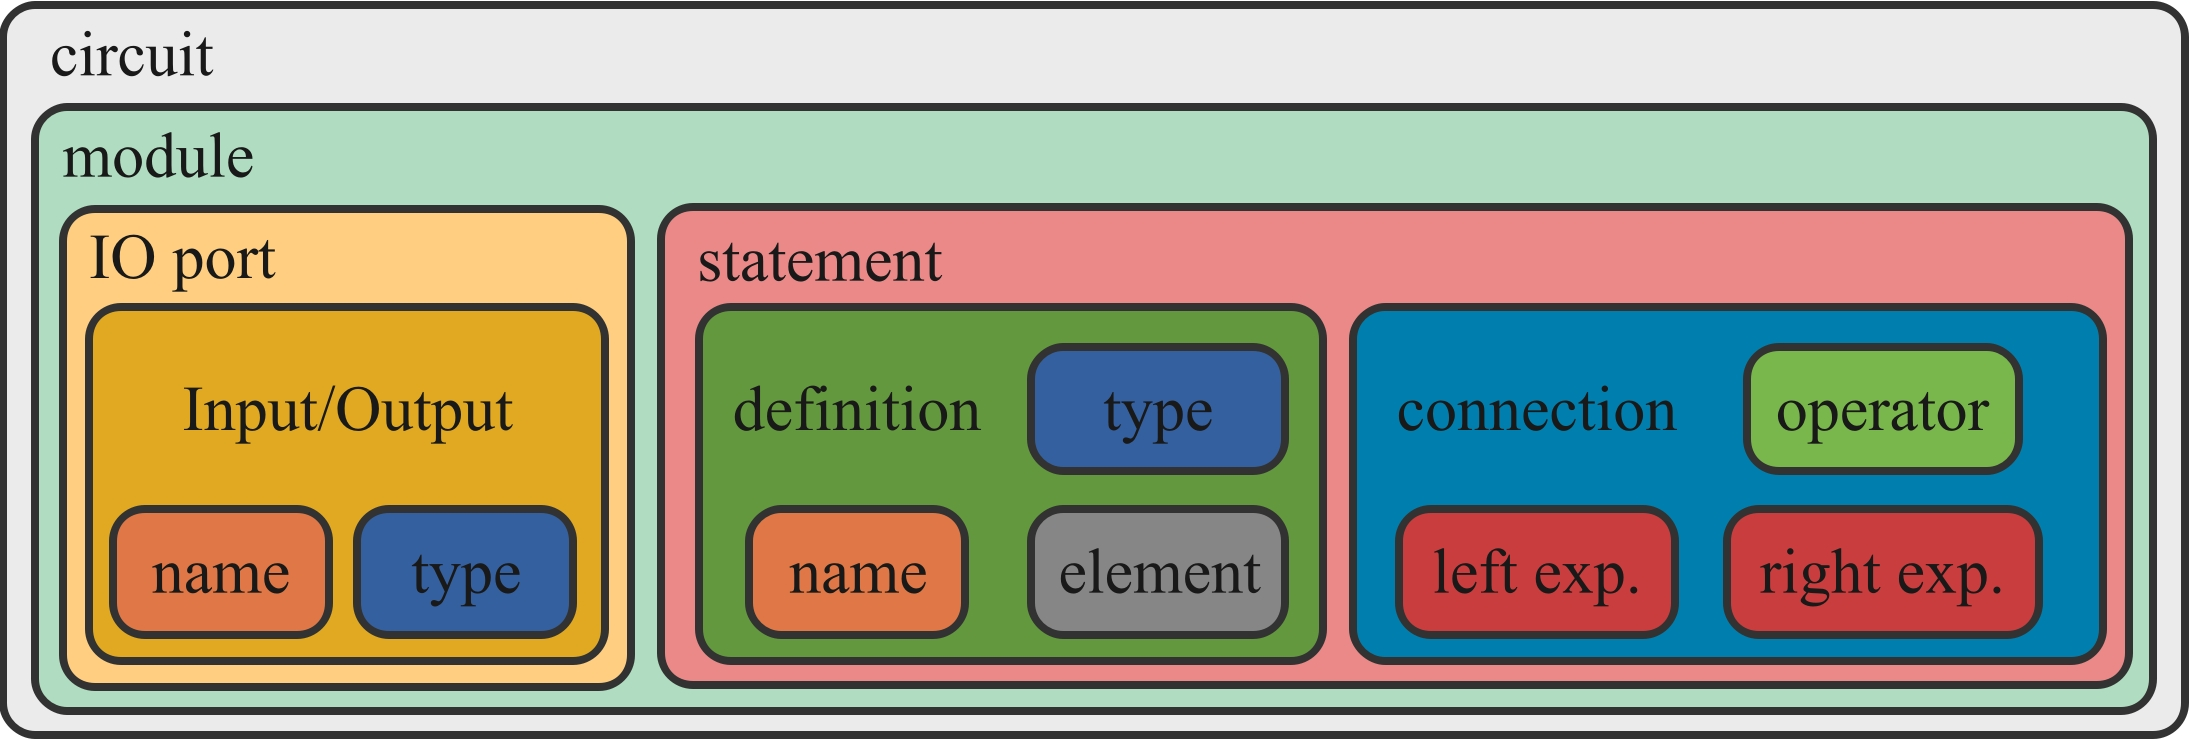
\includegraphics[width=0.95\textwidth]{Photos/PyHCL_IR-Structure.jpg}
	\caption{PyHCL IR的层次化节点设计}
\end{figure}

\begin{figure}[htbp]
	\centering
	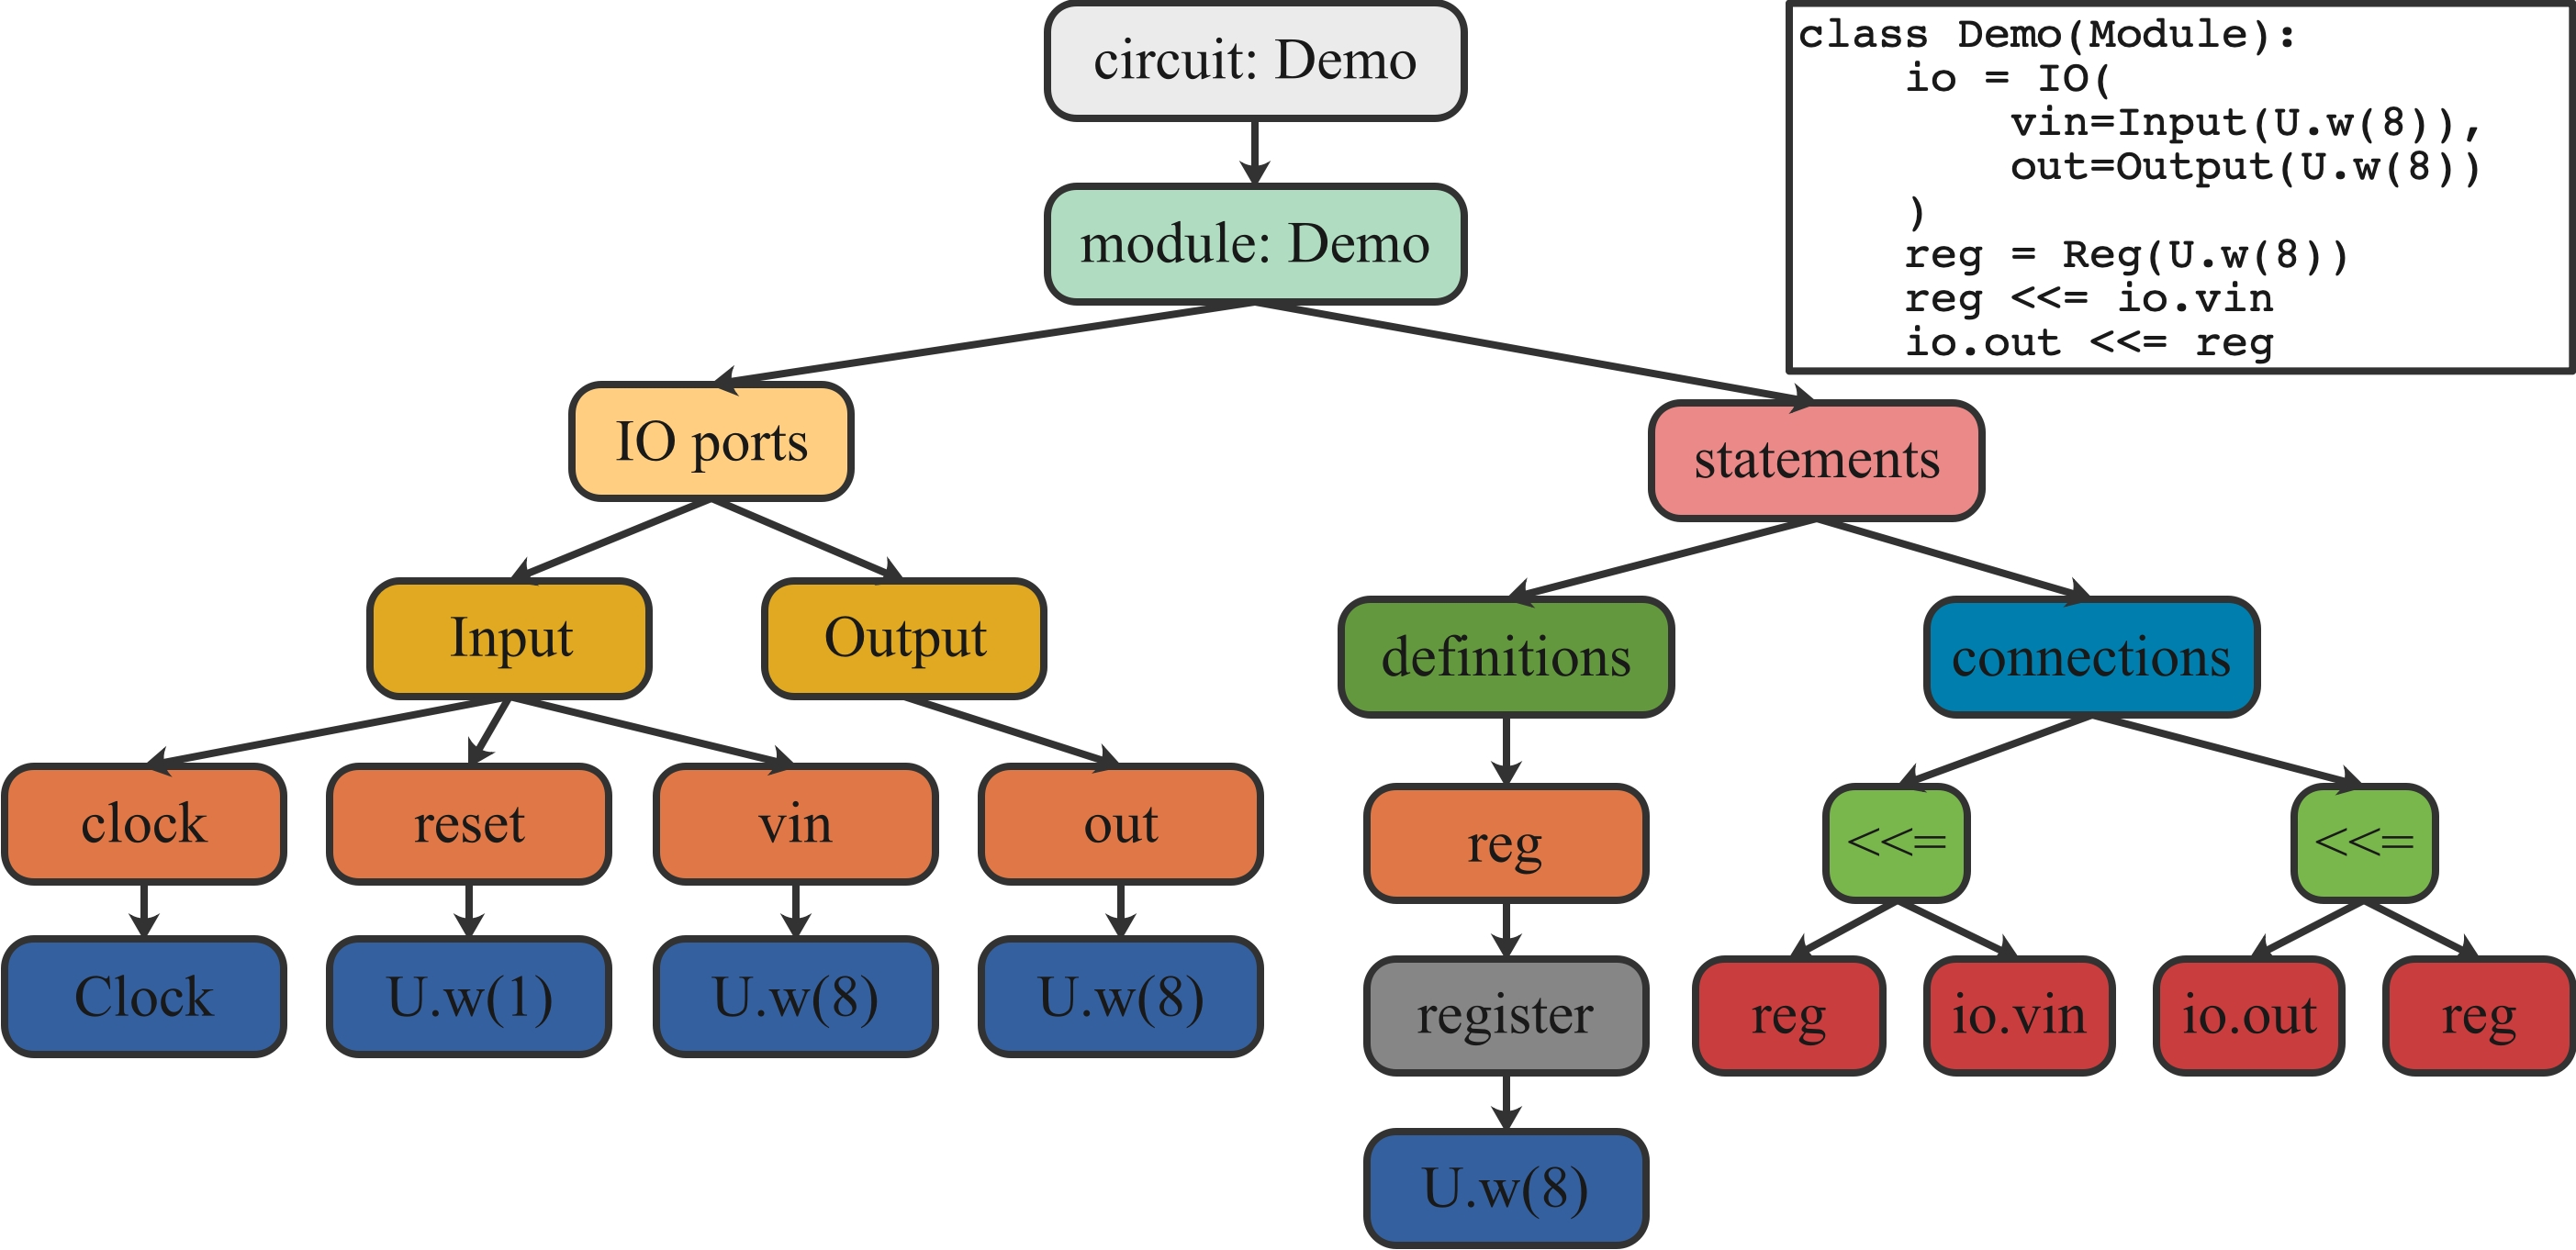
\includegraphics[width=0.95\textwidth]{Photos/PyHCL_IR-Example.jpg}
	\caption{一个PyHCL电路设计使用PyHCL IR节点表示的语法树形式的例子}
\end{figure}

一个典型的PyHCL电路设计通常包含多个PyHCL模块,为了简便起见,图2-3中的例子使用单个模块来作为例子。在多模块的设计当中,顶层模块将同时作为circuit节点。一个PyHCL模块包括两个部分:IO端口以及若干语句块。需要注意的是,PyHCL默认在每个模块构造的过程中自动生成隐式的时钟以及复位端口。PyHCL的语句块包括定义语句以及连接语句。对寄存器、线网以及存储器的定义即为定义语句,同时,在模块内实例化其他模块的语句也是定义语句的一种。对于连接语句来说,PyHCL IR规定连接运算符只能在两个合法的表达式节点之间使用。一个合法的表达式可以是单一的电路实体元素、一个匿名的临时节点(、一个PyHCL内置的工具函数,或者一个返回PyHCL电路实体元素的Python函数。如果一个表达式包含多个运算符,则PyHCL IR会生成多个匿名的临时节点来表示中间结果。PyHCL内置多种提高电路设计效率的工具函数,如Mux以及LookUpTable,其行为与多路选择器的功能类似,且可以接受Python列表或者集合作为输入。在PyHCL中应用函数式编程时,通常会使用高阶函数对寄存器向量或者存储器进行操作,并返回一个PyHCL电路元素实体,如2.1节中的FIR滤波器示例代码中的reduce函数。

从PyHCL代码转换为FIRRTL代码的过程主要是中间语法树生成的过程。PyHCL中负责构造语法树的elaborate函数首先将最顶层的模块作为入口,也就是语法树最顶层的circuit节点,自上而下的构造语法树,而对于以连接运算符为顶层节点的子树,构造的方式则是自底向上进行构造。对于每个模块,首先构造模块对应语法树上的IO端口,一般来说IO端口可以直接将其方向、名字、数据类型以及位宽映射到语法树当中,对于多层级的Bundle IO,则通过递归搜索每个子IO集合的方式来实现。定义语句的构造同样可以直接将电路实体元素类型、名称、数据类型以及位宽映射到语法树当中。对于连接语句,PyHCL通过对连接运算符的左右表达式应用后向搜索算法来构造语法树,如图2-4所示。

\begin{figure}[htbp]
	\centering
	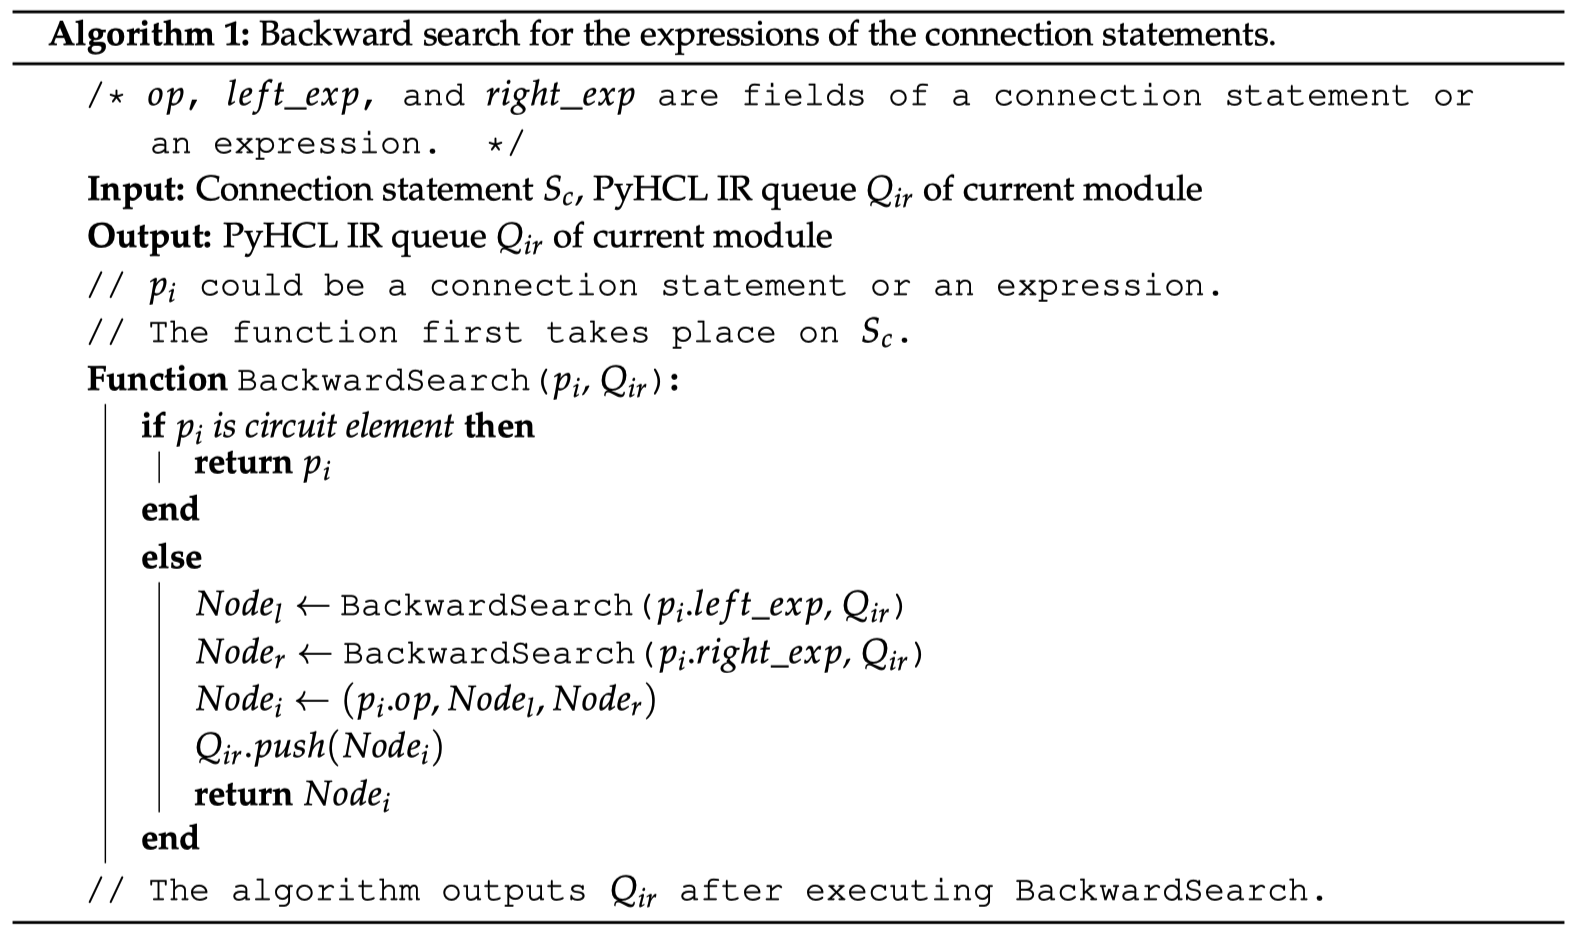
\includegraphics[width=0.95\textwidth]{Photos/back-end_search.png}
	\caption{构造连接语句语法树的后向搜索算法}
\end{figure}

图2-5给出一段连接语句的例子来说明构造PyHCL IR中间语法树的具体过程。

\begin{figure}[htbp]
	\centering
	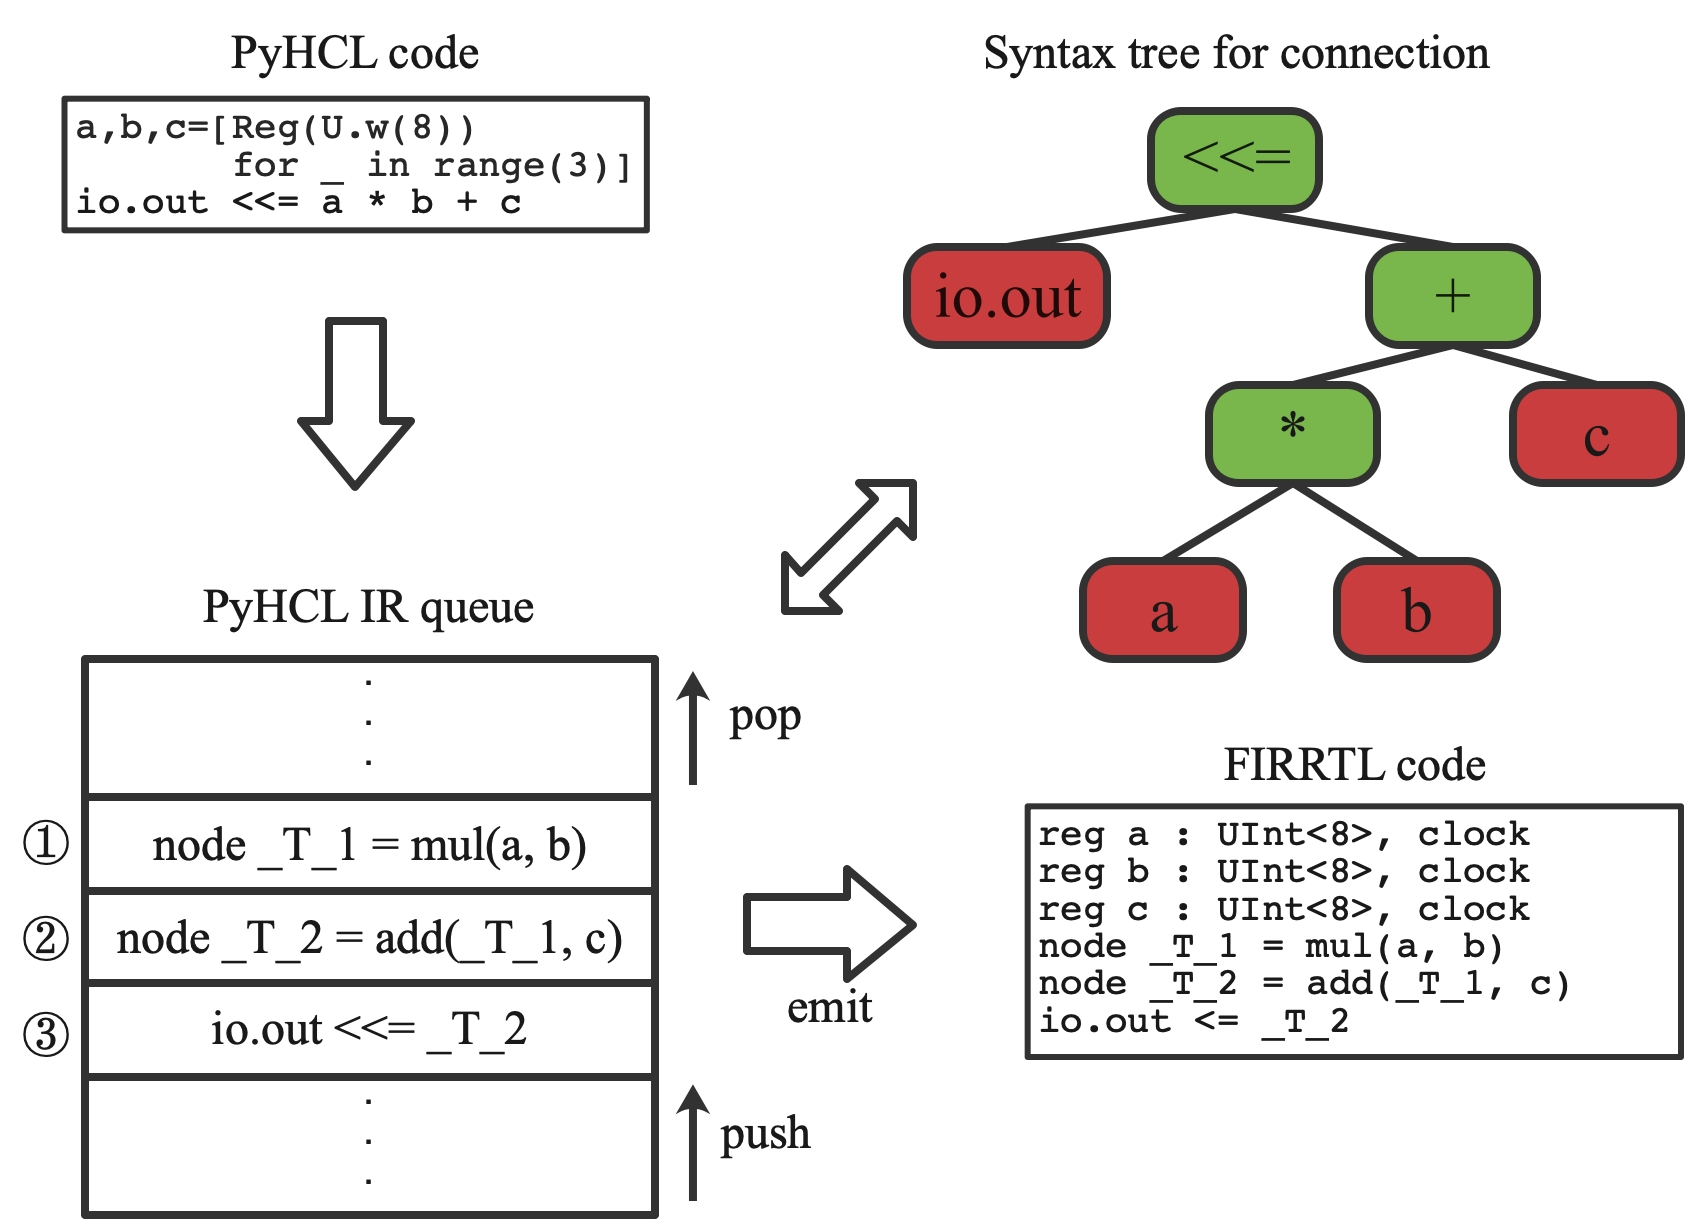
\includegraphics[width=0.95\textwidth]{Photos/Connections-backwared_search.jpg}
	\caption{连接语句的PyHCL IR中间语法树的构造过程}
\end{figure}

PyHCL IR中间语法树在内存中以队列的形式存在,每个PyHCL模块都包含一个PyHCL IR节点的队列。假设一个连接语句$io.out <<= a*b+c$,如图2-5所示。a、b和c都是存储8位无符号数的寄存器,根据运算符的优先级以及图2-4所示的后向搜索算法,语法树的构造过程首先从子表达式$a*b$开始,由于a和b都是叶节点,因此创建一个匿名临时节点$\_T\_1$并压入IR队列当中。接着返回到上一层的调用,对+运算符来说,右表达式寄存器c也是一个叶节点,因此创建第二个匿名临时节点$\_T\_2$,表示$\_T\_1$与c相加的逻辑节点并压入队列中,最后再将连接运算符节点本身压入队列当中。因此对于连接语句的子语法树构造,则是自底向上进行的,其在内存当中的表现形式则是1-3的节点序列,可以发现节点序列实际上就是语法树的前序遍历形式。图2-5中的例子实际上是从2.1节FIR滤波器例子中提取的基本MAC运算逻辑,如果将两个map、reduce高阶函数进行展开,则两个寄存器向量taps以及consts中的每个寄存器都会执行相同的MAC操作:$acc_i <<= taps[i] * consts[i] + acc_{i-1}$。

在构造连接语句的中间语法树过程当中,PyHCL还会进行数据类型检查以及位宽检查与推断的操作。如果左表达式与右表达式的数据类型不一致,则会抛出异常。如果表达式中存在没有显式声明位宽的寄存器或者线网,PyHCL会根据该寄存器或线网参与的连接操作推断其最小合法位宽。如果右表达式驱动的信号位宽大于左表达式的信号位宽,则会抛出异常。需要注意的是,如果一个参数化生成器的可配置参数用于表示位宽信息,则该参数同样会参与到位宽检查与推断的操作当中。这种策略可以将可能的位宽、数据类型违例检查提前进行,而避免电路设计一直到逻辑综合阶段才使用综合器来进行检查。同时,如果一个在定义语句中出现的电路实体元素节点没有出现在任何一个连接语句的左右子树当中,则该节点会被剔除,以此达到消除冗余元素的效果。

在构造当前模块语法树的过程中,如果遇到了子模块的构造声明语句,则会进入对该子模块的递归搜索当中,并返回表示该子模块语法树的队列。在完成了所有模块的语法树构建后,PyHCL生成器会将表示语法树的队列中的节点一一弹出,每个节点都包含有对应的合法FIRRTL语句块,如图2-5所示,并最终生成对应PyHCL电路的FIRRTL代码。

\section{使用FIRRTL构建PyHCL后端}

PyHCL与其他硬件生成框架相比,另一个显著的差异是PyHCL的后端生成目标语言是FIRRTL。大多数现代的硬件生成框架,例如MyHDL与PyRTL,它们的目标生成语言是Verilog,这种HGF称为基于Verilog的HGF。对于基于ASIC后端的集成电路开发流程来说,网表是介于前端RTL级Verilog代码以及后端设计流程(Place \& Route,P\&R)之间的中间表达形式。网表通常在RTL级Verilog代码完成验证工作后通过逻辑综合器生成。网表通常能够保留Verilog代码中的实现细节,换句话说,当Verilog代码能够维持一个相对稳定的电路功能结构时,后端的设计流程就可以更早地介入。如果网表结构在后续的开发迭代流程中发生了重大的改变,那么已经提前完成的后端流程将会浪费掉。基于Verilog的HGF不能够精确的操纵所生成的Verilog代码所表示的电路结构,这是因为这些HGF大都有黑盒制,且这些HGF在进入逻辑综合阶段前都无法地得到网表的任何信息。对于使用基于Verilog的HGF电路设计而言,一些针对原始电路逻辑的细微调整都有可能给生成的Verilog代码结构产生可观的改变,因此这也会导致对网表逻辑结构的改变。因此,使用基于Verilog的HGF进行电路设计,在进入后端P\&R阶段的网表必须保证稳定且尽量不变,否则修改设计所带来的成本将会非常高。

对于PyHCL来说,其后端生成目标语言是FIRRTL,而不是Verilog。FIRRTL具有更接近于网表结构的形式:LoFIRRTL。FIRRTL编译器支持FIRRTL向LoFIRRTL的转化,LoFIRRTL保持了原始FIRRTL的原语但将其转换为更为等效的但更简单、低抽象级别的电路结构。换句话说,LoFIRRTL所表示的电路结构更接近于网表模型。只要PyHCL设计可以保证LoFIRRTL的稳定性,则可以维持该设计所对应的网表结构保持不变。图2-6展示了FIRRTL代码及其对应的LoFIRRTL形式,以及编译后生成的可综合Verilog代码。FIRRTL代码的例子来源于图2-5中的MAC运算。

\begin{figure}[htbp]
	\centering
	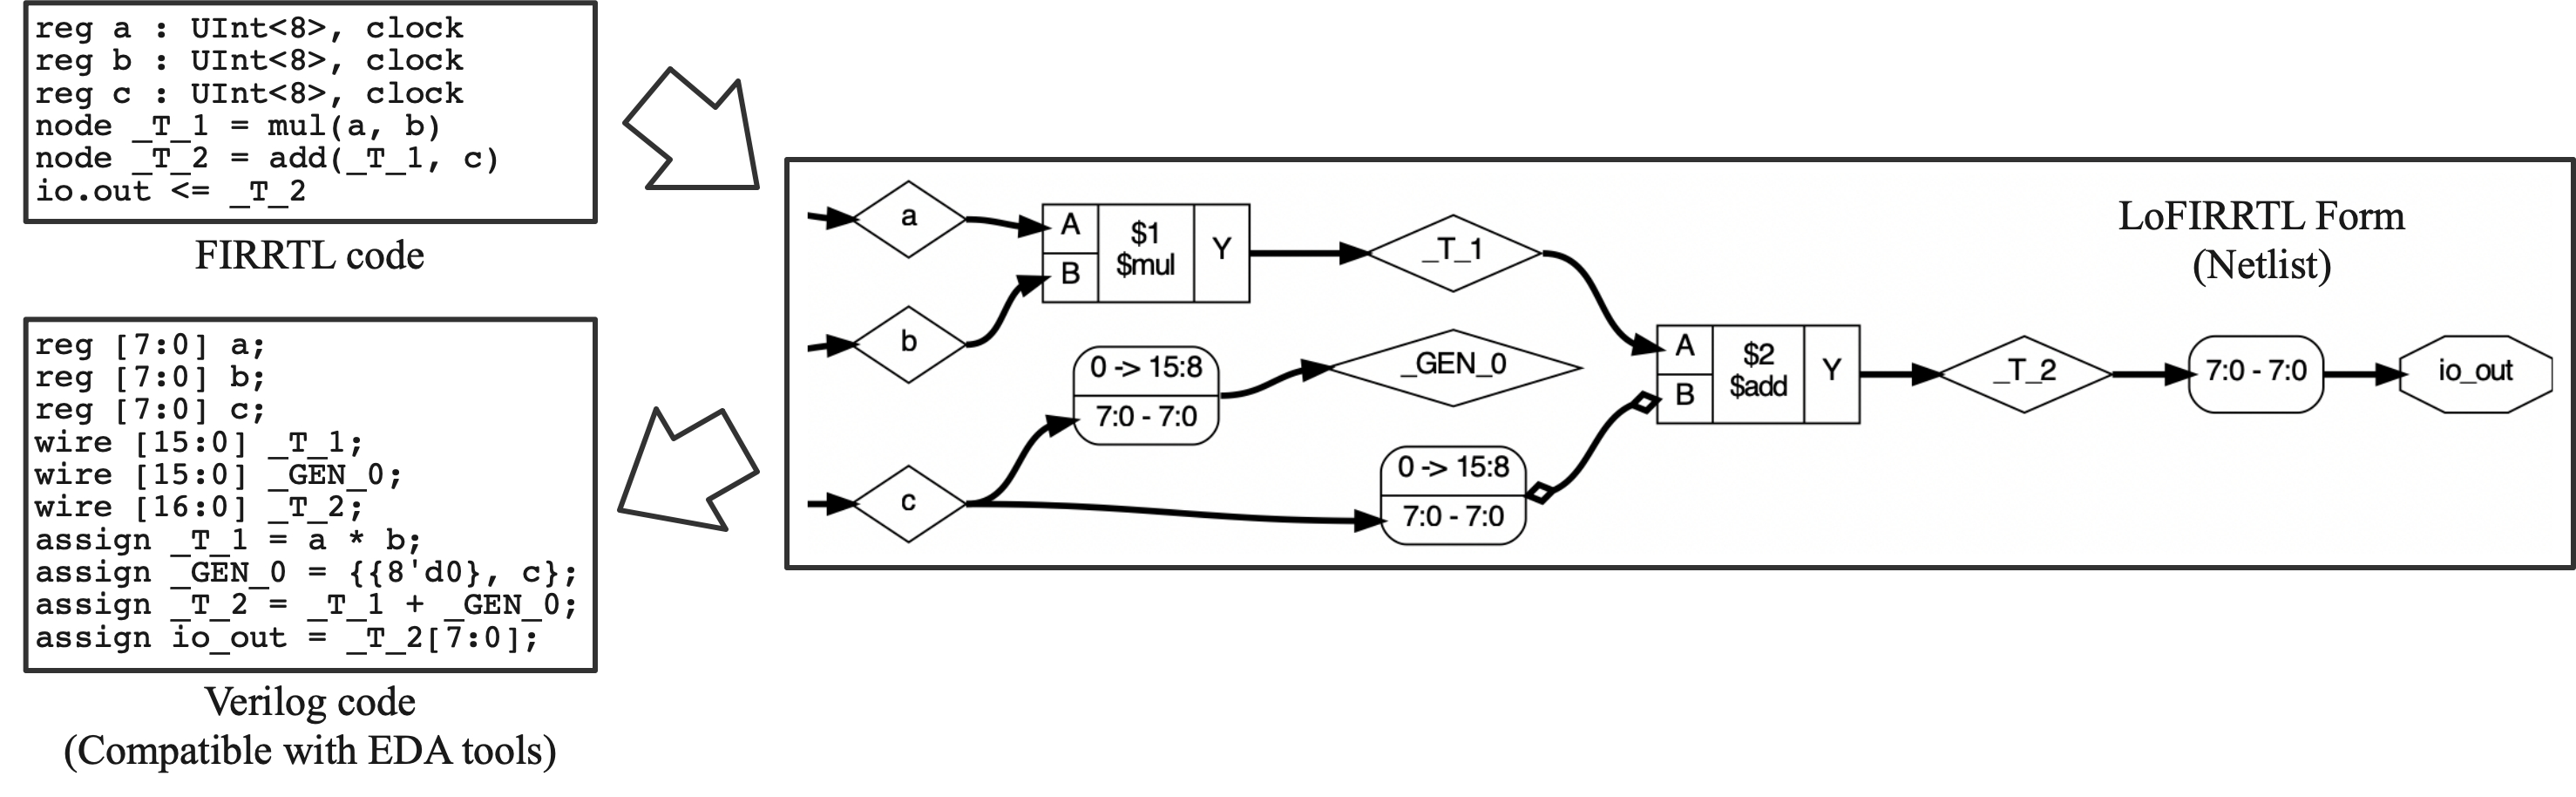
\includegraphics[width=0.95\textwidth]{Photos/FIRRTL_intro.jpg}
	\caption{FIRRTL代码及其对应生成的LoFIRRTL形式、Verilog代码}
\end{figure}

在2.2节提到过,PyHCL中间语法树的IR节点是与FIRRTL原语紧耦合的,这意味着设计者可以通过PyHCL代码精确的控制所生成FIRRTL代码所对应的LoFIRRTL网表结构。因此,使用基于PyHCL进行的硬件设计流程可以将后端P\&R流程尽可能的提前,缩短开发迭代周期,且开发者能够在FIRRTL层级上完成工程改变命令(ECO,Engineering Change Orders)。此时在后续迭代周期中新添加的功能可以通过检查设计所对应的LoFIRRTL网表模型是否有显著改变,来防止浪费上一个迭代周期已完成的后端流程工作。

除此之外,FIRRTL还提供了针对不同FPGA平台宏定义的抽象表达形式,比如不同FPGA平台对平台内置存储器的宏定义。PyHCL设计代码可以通过FIRRTL来保证对包括不同FPGA平台甚至ASIC工艺库的兼容性。综上所述,PyHCL可以显著的缩短硬件开发的迭代周期,并进一步实现硬件敏捷设计的目标。

\section{本章小结}

本章对基于Python的硬件全栈设计框架PyHCL进行的介绍,对PyHCL的接口、中间语法树IR、生成器(emitter)以及PyHCL后端生成的FIRRTL语言进行了介绍。PyHCL通过其独有的函数式编程以及参数化生成器特性,与传统的硬件描述语言以及其他硬件生成框架所区别开来,能够允许用户快速创建电路设计原型并快速迭代,达到硬件敏捷设计的效果。同时,PyHCL的后端FIRRTL语言能够使用户在LoFIRRTL类网表结构上提前进行后端流程,并在LoFIRRTL上完成ECO,以达到加快开发迭代周期的效果。
%第二章
	\chapter{面向DSP的嵌入式微处理器设计与实现}

本章节对本文所实现的基于RISC-V的面向DSP的嵌入式微处理器进行介绍。本文所实现的微处理器主要应用场景为物联网设备、移动终端等需要满足低功耗前提,同时具有一定计算能力的设备。本文所实现的微处理器具有以下的特性:

\begin{enumerate}
	\item 实现了RISC-V中的RV32GCP指令集,即实现了32位整数指令集“I”、乘除指令集“M”、原子操作指令集“A”、单精度浮点指令集“F”、双精度浮点指令集“D”、压缩指令集“C”以及专为DSP运算增强的SIMD指令集“P”[40]。
	\item 微处理器的流水线基本框架参考了CV32E40P开源微处理器的实现,微处理器流水线采用单发射顺序执行4级流水线设计,4个流水级分别为取指(IF)、译码(ID)、执行(EX)以及写回(WB)。除了加载指令以及需要写回寄存器组的指令外,都在执行阶段完成并提交。对于存储器相关指令,则提交给加载存储单元(Load Store Unit,LSU)执行,LSU通过核内自定义的总线协议与缓存交互。
	\item 微处理器中“P”指令集采用了并行多数据通路的策略实现,通过扩展译码器以及ALU的方式实现SIMD相关指令。微处理器软核IP中可以根据实际应用需要,通过配置不同的参数生成带有“P”指令集扩展的RTL代码或仅支持RV32GC基本实现的RTL代码。
	\item 微处理器核仅实现了机器模式的特权级架构,并实现了核内本地中断控制器CLINT(Core Local Interrupt Controller)以提供带优先级的可抢占式中断服务。
	\item 微处理器外围适配的SoC片上系统实现了RISC-V Debug调试模块以及串口、GPIO、I2C、SPI等外部总线,片上总线使用AMBA AXI4总线协议,对于低速的外设,则使用低功耗的APB总线协议。APB与AXI4之间协议通信通过APB桥进行转换。
\end{enumerate}

微处理器RTL级描述完全通过PyHCL实现并验证,并通过riscv-tests[41]测试。以该微处理器为内核的SoC片上系统在Xilinx N4 FPGA平台上成功部署并进行CoreMark[42]性能测试。本章节将从以下四个方面对微处理器的实现进行介绍:流水线具体实现、特权模式实现、“P”指令集实现以及SoC片上系统实现。在本章节的最后给出微处理器的相关测试数据。图3-1给出包含该微处理器内核的SoC片上系统的概览。

\begin{figure}[htbp]
	\centering
	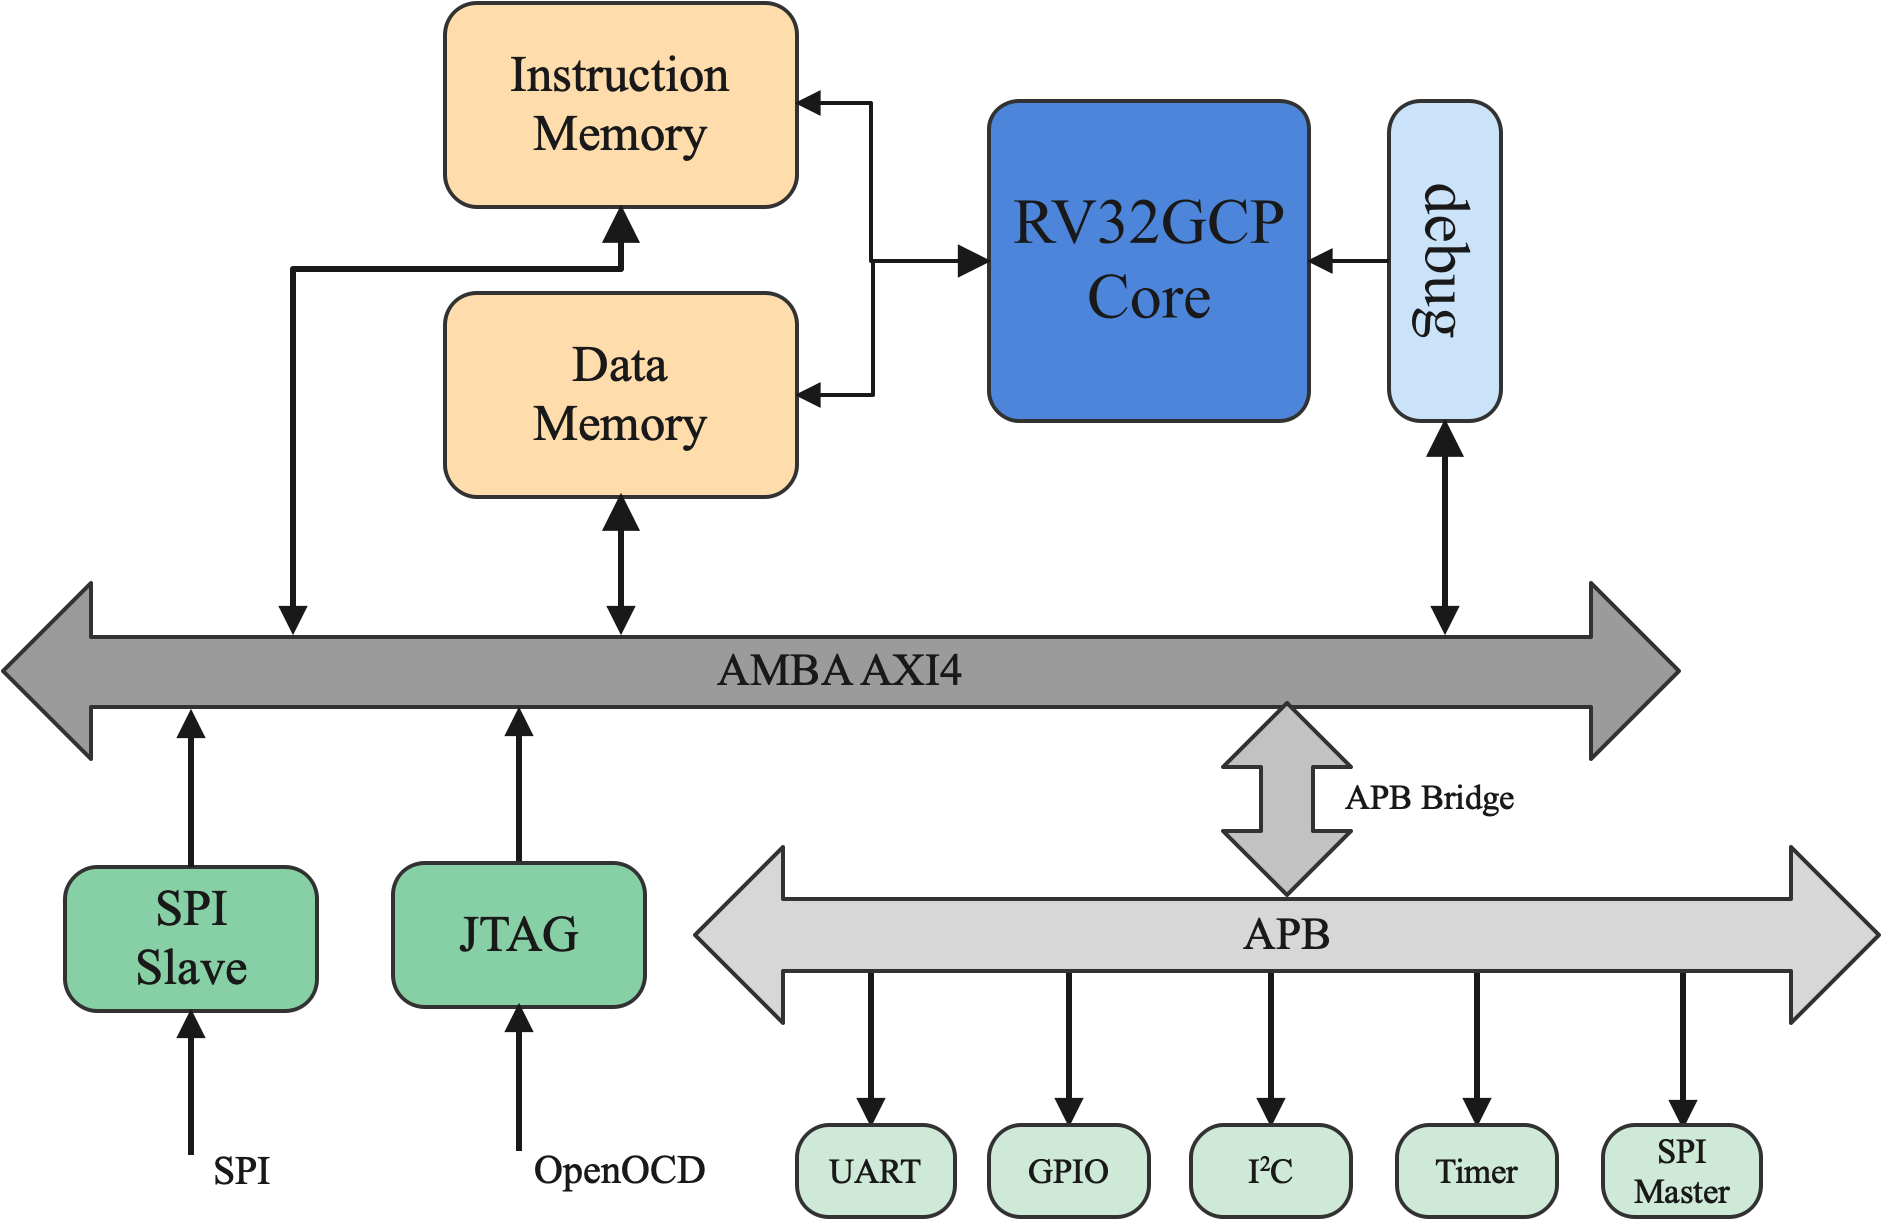
\includegraphics[width=0.95\textwidth]{Photos/SoC_Overview.png}
	\caption{包含RV32GCP RISC-V内核的SoC片上系统结构}
\end{figure}

\section{微处理器流水线细节}
\subsection{流水线概览}

基于性能以及功耗的综合考虑,本文的微处理器实现使用了单发射的顺序流水线结构,而非高性能微处理器中常用的顺序多发射超标量乱序执行处理器的结构。后者一般使用较为激进且复杂的分支预测策略以及托马苏洛算法[43]与重排序缓冲区来实现乱序执行,这种结构在性能上虽然比顺序发射执行的单发射流水线要好,但芯片整体的面积以及功耗无法达到嵌入式设备的需求。微处理器流水线的整体结构如图3-2所示。

\begin{figure}[htbp]
	\centering
	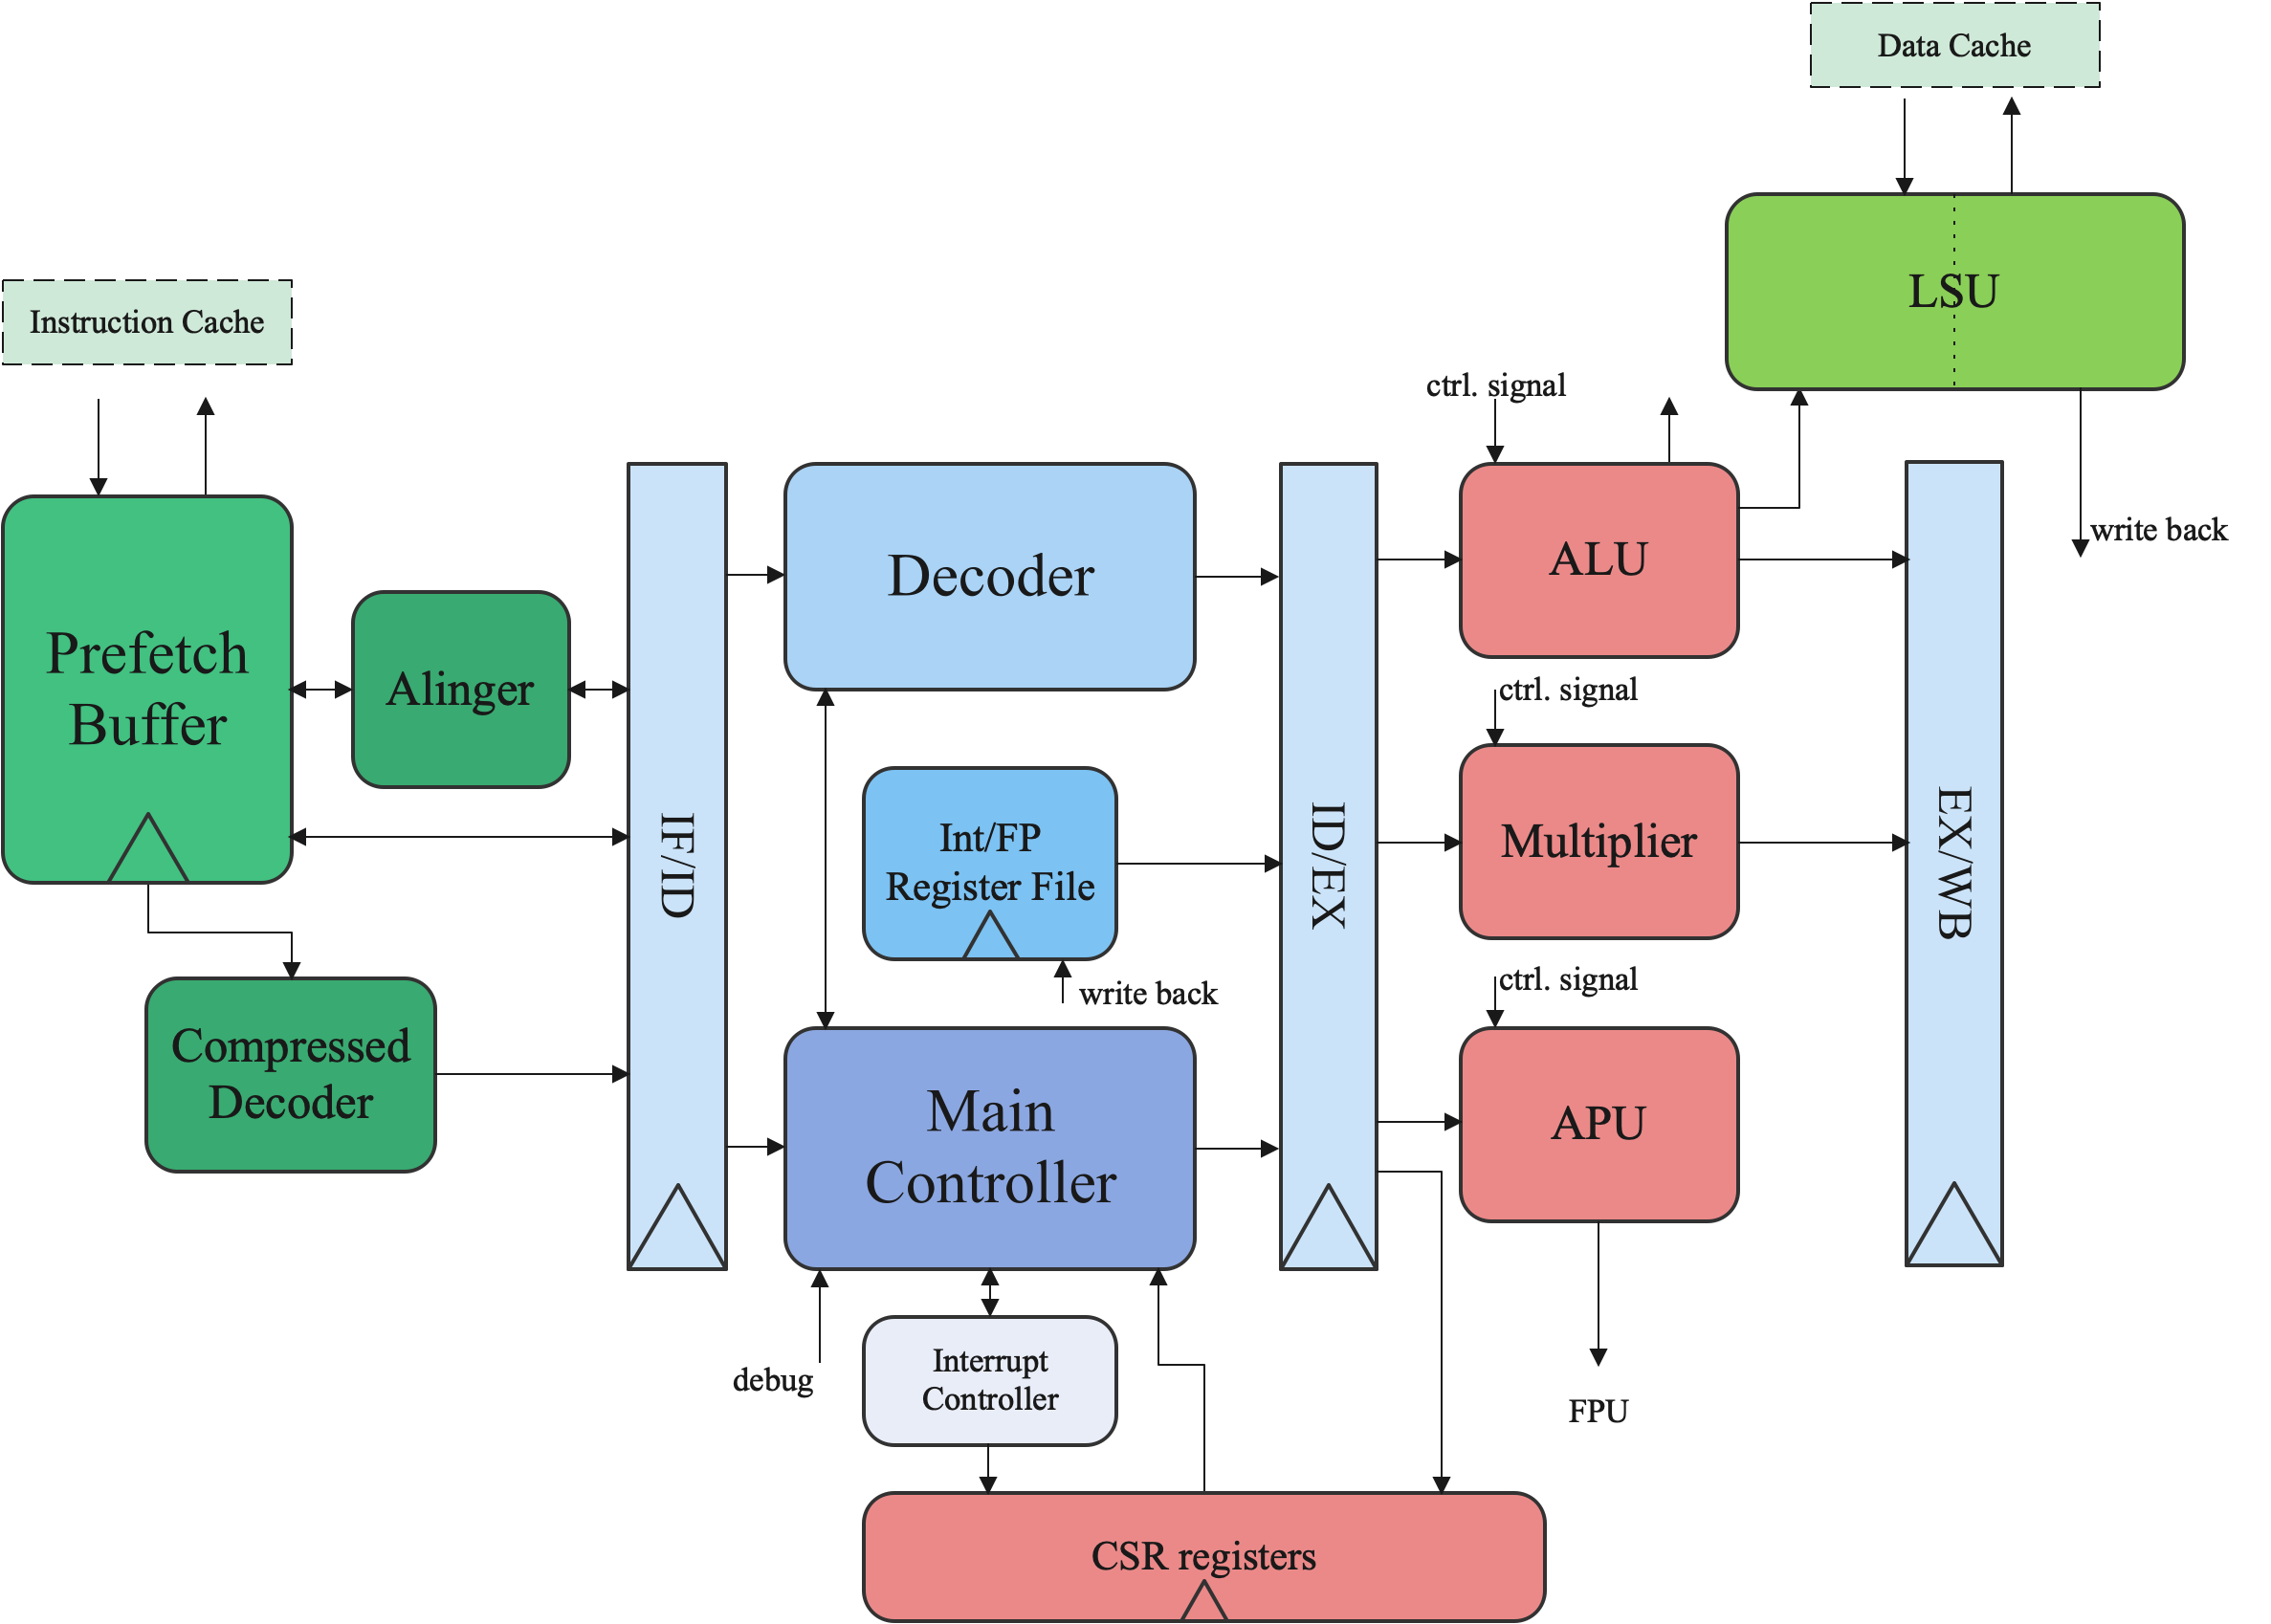
\includegraphics[width=0.95\textwidth]{Photos/Pipeline.png}
	\caption{微处理器流水线整体结构图}
\end{figure}

微处理器中4个流水线级的主要功能及作用概述:

\begin{enumerate}
	\item 取指阶段(Instruction Fetch,IF)。取指阶段通过核内自定义的总线协议(与LSU总线协议相同)从最低级的指令L1缓存中取指,并保存在一个小的预取缓冲区当中。预取缓冲区可以缓解因非对齐的指令地址所造成的停顿问题。同时取指阶段也会对16位的压缩指令进行预先的译码,转换为标准的32位RISC-V指令集传递到译码阶段。分支预测单元也包含在取指阶段当中。
	\item 译码阶段(Instruction Decode,ID)。译码阶段对取指阶段中的指令进行译码,并转化为若干控制信号控制微处理器中各功能单元的执行。译码阶段包含有译码器、主控制器以及中断控制器,其中无条件跳转指令在该阶段执行。
	\item 执行阶段(Execute,EX)。执行阶段包括执行指令所需要的功能单元:算术逻辑单元ALU、乘除法器以及协处理器接口单元APU。考虑到浮点运算功能实现的复杂度以及延迟,浮点功能通过APU与核外的浮点运算单元交互来实现。有条件跳转指令在该阶段执行,通过ALU对跳转条件进行判断,并将结果反馈到主控制器来控制是否进行分支。部分指令在执行阶段需要多个周期完成,对于多周期的指令,微处理器一律通过停顿来保证不会出现数据冒险。所有需要写回寄存器的算术逻辑指令在该阶段即完成写回操作。同时,针对存储器相关指令的地址也会在执行阶段生成,并传递给LSU。
	\item 写回阶段(Write back,WB)。写回阶段只对于加载指令有效,所有加载指令的写回在该阶段完成。这是因为通过自定义的总线协议从最低级的数据L1缓存中加载指令至少需要1个周期的时间才能返回数据。
\end{enumerate}

表3-1展示了微处理器中除浮点以及“P”扩展以外指令的周期数,所有执行周期大于1的指令都会导致流水线停顿并带来CPI(指令平均执行周期数,Cycle Per Instruction)的损失。

\begin{table}
	\caption{指令类型及其对应的执行周期数}
	\centering
	\small 
	\begin{tabular}{p{80pt}p{50pt}p{200pt}}
		\hline 
		指令类型 & 执行周期                & 备注             \tabularnewline
		\hline 
		RV32I 算术逻辑运算   & 1		     & 基本的RV32I算术逻辑运算只需要1个周期完成 \tabularnewline
		整数乘法   & 1或5	     & mul指令只需要1个周期,mulh、mulhsu、mulhu需要5个周期完成 \tabularnewline
		除法/取模   & 3到35	     & 除法与取模所需要的周期数取决于被除数前导零的个数 \tabularnewline
		无条件跳转   & 2     & 无条件跳转在ID阶段执行 \tabularnewline
		有条件跳转   & 1或3     & 不进行分支的有条件跳转不会带来停顿,进行分支的有条件跳转需要刷新IF及ID阶段。分支预测错误的跳转指令也需要3个执行周期。 \tabularnewline
		CSR访问   & 1或4     & 访问不同的控制状态寄存器需要不同的周期,具体定义在RISC-V的Zicsr指令集中 \tabularnewline
		加载/存储指令   & 1或2     & 对齐的加载/存储指令需要只需要1个周期,非对齐或者半字(16位)的加载/存储指令需要2个周期。 \tabularnewline
		\hline 
	\end{tabular}
\end{table}

微处理器实现中对冒险(Hazard)的处理如下:

\begin{enumerate}
	\item 对于结构冒险,由于多周期的指令一律通过流水线停顿处理,因此流水线中不存在同一周期中出现冲突的功能单元,不存在结构冒险。
	\item 对于数据冒险,由于流水线是顺序执行的,因此只存在写后读(RAW)冒险,不存在读后写(WAR)以及写后写(WAW)的数据冒险。对于写后读的数据冒险,主要通过旁路转发的方式进行处理,以尽可能的提高CPI。但仍存在两种情况需要停顿1个或多个周期来解决数据依赖:加载数据冒险,即紧跟在一条加载指令后的指令依赖于加载指令的目标寄存器数据;基于寄存器的链接跳转指令jalr的数据冒险,即一条jalr指令依赖于上一条指令的目标寄存器数据。
	\item 对于控制冒险,无条件跳转指令固定具有1个周期的惩罚,这是因为无条件跳转都在ID阶段执行,此时已经进入IF阶段的指令都会被刷新。有条件跳转取决于两个因素:是否执行分支以及分支预测是否正确。不执行的分支以及错误的分支预测都会导致已经进入IF、ID阶段的指令被冲刷掉,带来2个后期的惩罚。可以看出,有效的分支预测策略可以为CPI带来显著的提升。
\end{enumerate}

\subsection{取指阶段}

取指阶段将从最低级指令L1缓存中获取指令,并存储到预取缓冲区或直接传递给ID阶段,同时对压缩指令进行预先译码转换成32位标准指令传递给ID阶段。取指阶段还会对非对齐的指令地址访问进行处理。取指阶段的主要模块及其功能如下:

\begin{enumerate}
	\item 预取缓冲区:预取缓冲区可以实现对非对齐指令的单周期取指,以优化流水线的整体性能,其整体结构为一个先进先出的队列。
	\item 取指地址对齐单元:由于预取缓冲区请求的指令地址永远是32位对齐的,但本文实现的微处理器支持16位压缩指令,因此在指令L1缓存中混合有32位及16位的指令。取指地址对齐单元则用于处理非对齐指令读取的情况。
	\item 压缩指令译码器:将16位的RISC-V压缩指令译码为32位指令。
\end{enumerate}

预取缓冲区设计的主要目的是为了降低非对齐指令访问的延迟。如果不做任何处理,非对齐的指令访问需要2个时钟周期才能取得。预取缓冲区的默认大小为4个字节,即128位,可以保证在不占用过多面积的同时提升性能。下面以一个例子来说明预取缓冲区的设计如何实现非对齐指令的单周期取指。

如图3-3所示,假设当前PC指向地址为0x80的32位数据,其中低16位是压缩指令,而高16位是下一条32位指令的前16位。此时地址为0x84的32位数据已经被预取到预取缓冲区当中,因此首先将压缩指令传递到压缩指令译码器中译码并送至ID阶段,同时该32位的数据还会保存在取指地址对齐单元的寄存器中保留多一个时钟周期。下一个周期,PC指向变为0x84,则从预取缓冲区中直接读取下一个指令的高16位部分,并与上个周期的32位数据的高16位组成一个完整的指令传递给ID阶段,即可达到对非对齐的指令实行单周期读取的效果。如果没有预取缓冲区,则IF阶段需要发送非对齐的地址至指令L1缓存,指令L1缓存则需要分成2个周期来传送该指令,因此,预取缓冲区还可以使取指地址固定32位对齐,而不需要考虑压缩16位压缩指令与32位指令混合的情况。

\begin{figure}[htbp]
	\centering
	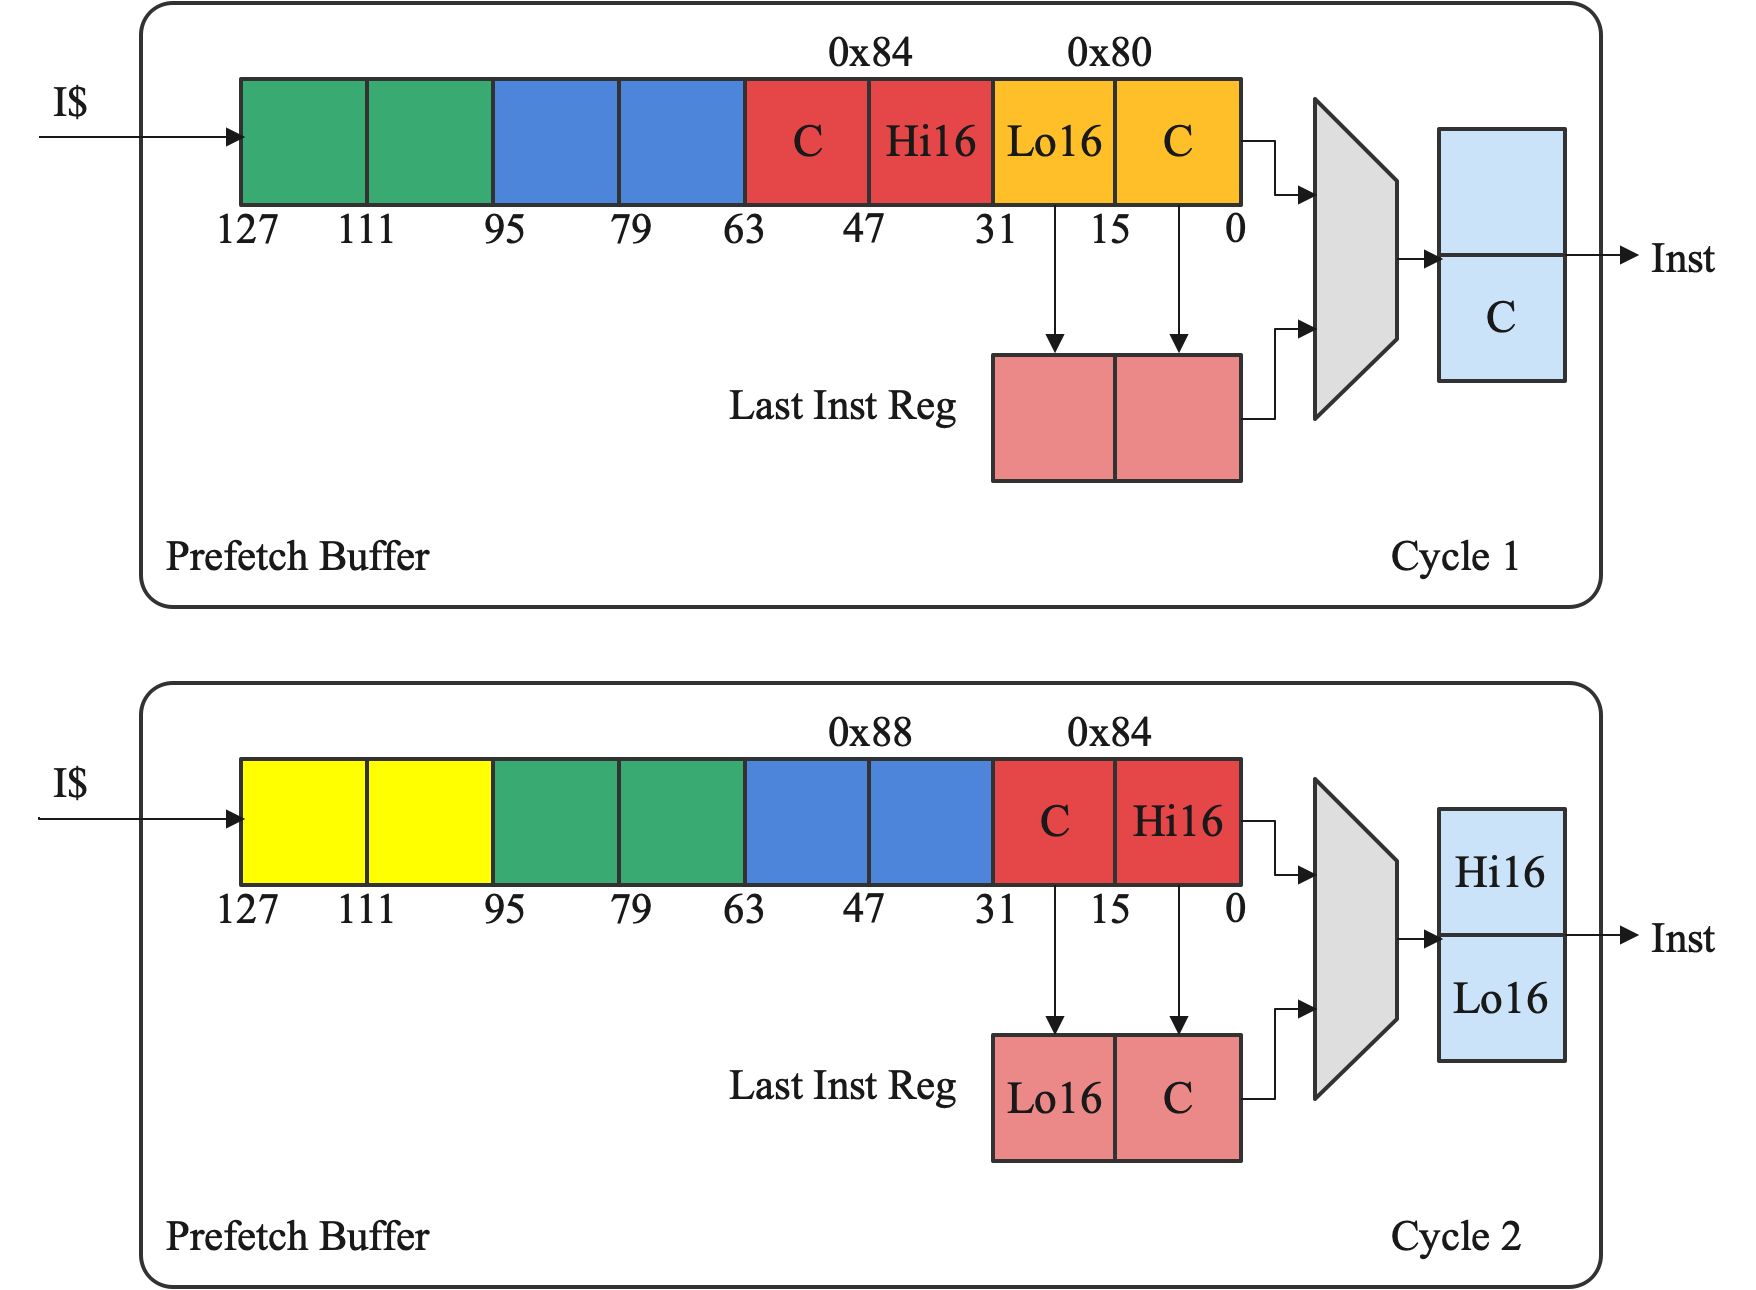
\includegraphics[width=0.95\textwidth]{Photos/PrefetchBuffer.png}
	\caption{单周期非对齐指令读取示例。其中“C”表示16位的RV32C指令,“Hi16”表示32位RISC-V指令的高16位,“Lo16”表示32位RISC-V指令的低16位。}
\end{figure}

取指地址对齐单元与预取缓冲区功能互相配合,其内部是一个状态机,状态机的状态主要取决于上一周期从对齐地址取回的32位数据及当前周期从对齐地址取回的32位数据内容情况,同时还要考虑当跳转指令目标地址也是非对齐情况时的处理,如跳转指令的目标地址也是一个16位的压缩指令。

压缩指令译码器是纯的组合逻辑结构,其功能仅简单的使用多个多路选择器将压缩指令译码为32位指令。

除此之外,取指阶段还包含有一个简单的分支预测器。分支预测器使用基于4K大小动态分支缓冲区的两位饱和计数器策略来预测分支是否执行,在保证面积优化的同时提高流水线的性能。对于目前较为流行的数种不同的分支策略,在权衡利弊后作出了如上选择,原因在于:

\begin{enumerate}
	\item 一个简单的使用4K项缓冲区全局二位饱和计数器分支预测策略在SPEC89测试上的预测准确率可以达到82\%到99\%,这种简单且空间较小的预测器所实现的动态分支预测策略相比于每次进行分支都冲刷IF、ID的流水线级间寄存器对CPI性能的提升要好。同时相比于静态的分支预测,该策略仅使用较小的缓冲区代价就可以带来相当高的性能改善。
	\item 高级的分支预测器如相关分支预测器[44, 45]、竞赛预测器[46]、带标记的混合预测器[47]具有相当高的分支预测准确率,在SPECint测试上最高可以达到97.8\%到98.2\%的分支预测准确率。但这些分支预测器的实现逻辑非常复杂,在面向低功耗的嵌入式系统当中实现并不现实。
\end{enumerate}

\subsection{译码阶段}

译码阶段将来自取指阶段的指令进行译码操作,并转换为若干控制信号发送给相关的执行单元执行当前指令。译码阶段还包括从整数寄存器组以及浮点数寄存器组的读取操作。中断控制器用于外部中断的仲裁及CSR寄存器组的交互。无条件跳转在译码阶段进行,将IF/ID流水线间寄存器冲刷,给流水线带来固定1个时钟周期的延迟。译码阶段的主要模块及其功能如下:

\begin{enumerate}
	\item 整数及浮点数寄存器组:带有32个32位整数寄存器以及32个32位浮点数寄存器的寄存器组模块。在本文的实现中基于FPGA的后端工艺采用了触发器的实现。寄存器组带有3个读端口以及2个写端口,以保证不会出现结构冒险的情况。整数寄存器以及浮点数寄存器共享相同的旁路以及写入的逻辑。
	\item 译码器:纯组合逻辑单元,将来自取指阶段指令译码并将相关信息传递到主控制单元。如果指令是无效的,将会触发内部异常。
	\item 主控制单元:接收来自译码器以及其他功能模块、流水线间寄存器的反馈信号,根据内部状态机的转移发出相应的控制信号到各功能模块。主控单元同时还负责接收来自外部的调试信号,以控制流水线的启停。
	\item 中断控制器:接收外部中断信号并基于中断优先级进行仲裁,将仲裁结果反馈到CSR寄存器组。若中断使能且有效,则跳转到相对应的中断服务程序。
\end{enumerate}

译码阶段的主要工作是根据RISC-V指令集标准对指令进行译码操作,其硬件逻辑主要是由大量多路选择器所组成的选择逻辑结构,在此不对这方面进行过多的赘述。

\subsection{执行阶段}

执行阶段接收来自译码阶段主控制器的控制信号,并根据信号执行指令。执行阶段最主要的功能模块为算术逻辑单元ALU,ALU负责执行RV32I中的基本整数算术逻辑运算以及“P”扩展指令集中的SIMD运算。乘除法的实现相互分离,除法器使用基本的串行移位除法器实现,整合在ALU当中。乘法器则作为单独的功能单元与ALU分离。执行阶段还包含一个辅助处理单元(Auxiliary Processing Unit,APU)来实现与流水线外部FPU单元交互。状态控制寄存器组(Control Status Registers,CSRs)也包含在执行单元,对CSR的读写操作在执行阶段进行。对于除存储器加载以外的指令来说,写回的操作也发生在执行阶段,换句话说,从执行阶段开始会对微处理器架构状态发生改变。执行阶段的主要模块及其功能如下:

\begin{enumerate}
	\item 算术逻辑单元ALU:ALU主要由以下的部分组成:一个32位整数加法器,由4个先行进位8位加法器组成、移位及比较单元、串行移位除法器、以及用于“P”扩展指令集中SIMD指令及其他指令的执行单元。有关“P”扩展指令的实现将在3.3节中进行叙述。
	\item 乘法器:乘法器包括一个32位乘32位的整数乘法器,对于非取结果高32位的指令(mulh系指令)只需要1个时钟周期即可完成,否则则需要5个时钟周期。32位的整数乘法器通过分区的方式实现,以此方便对“P”扩展指令集中SIMD指令的实现。
	\item 辅助处理单元:辅助处理单元通过自定义的接口协议与浮点处理单元(FPU)交互。与一般的总线协议类似,辅助处理单元在地址阶段发送浮点操作数、浮点操作以及请求信号至FPU,FPU运算后的结果在响应阶段发回到辅助处理单元。
	\item 控制状态寄存器组:CSRs包含一系列保存有微处理器当前状态信息的寄存器组,如机器模式状态寄存器mstatus,其中包含有当前微处理器所处的特权级模式、各特权模式下的中断使能状态等。与通用寄存器组不同,CSRs的读写需要一定的权限,如用户模式下尝试对机器模式的控制状态寄存器进行读写会引发内部异常。
\end{enumerate}

根据表3-1中所提到的,乘法器执行32位乘32位的整数乘法,在只需要低32位的结果时只需要1个时钟周期,而需要高32位的结果时则需要5个时钟周期。这是因为在只需要低32位的mul指令时,乘法器直接调用32位乘法器计算得到低32位结果。而在需要高32位的结果时,乘法器则使用分区的16位乘16位乘法,在5个时钟周期中分时计算并取高32位结果输出。在RTL级的代码实现中,一个简单的“*”运算符在进行逻辑综合时会根据乘法运算位数而生成不同大小以及复杂度的乘法器,因此需要谨慎考虑进行乘法运算时操作数的位数。逻辑综合器一般会对乘法器做一定的优化,如基于Radix-4的booth编码乘法器[48]、基于保留进位加法器的华莱士树等等,具体的优化策略根据综合时的约束综合器会生成不同的乘法器。

除法以及取模的运算需要最少3个时钟周期到35个时钟周期不等,这是因为除法器实现的是逻辑较为简单的串行移位除法器。除法器内部控制单元实现一个状态机,其中有3个固定的时钟周期用于启动以及结束运算,余下的为线性移位除法的运算周期。被除数的前导零越多,运算所需要的周期越少。与乘法不同,除法的优化空间不多,追求性能较高的除法器会牺牲大量的面积,因此在低功耗的微处理器实现中一般都使用较为简单的串行除法器。

外部FPU的设计采用参数化的设计方法,考虑到浮点运算的复杂性,FPU将浮点运算分为4大类来实现,分别为浮点加法与浮点乘法、浮点除法与浮点平方根、浮点比较、浮点与浮点/整数之间的转换。4大类运算使用并行的数据路径以及运算单元实现,且通过参数配置运算单元的流水级数。流水级数越少,运算所需要的时钟周期数越少,延时越低,但逻辑面积越大。

控制状态寄存器组的具体实现则遵循RISC-V特权级指令标准实现,在此不进行过多的赘述。

除此之外,还需要注意的一点是,在执行阶段ALU也会对存储器相关操作的地址进行运算并生成,提交到加载存储单元中,并向最低级数据L1级缓存发出请求。在下一个周期指令进入写回阶段,从缓存中读取的数据返回到LSU中,并写回到通用寄存器组。这就是为什么图16中LSU在结构上可以看作是横跨执行阶段以及写回阶段。

\subsection{写回阶段}

写回阶段主要是加载存储单元对从存储器读数据的阶段,即可以看作是内部总线协议的响应阶段。只有从存储器中加载数据到通用寄存器组的指令才会到达写回阶段。指令处于写回阶段的时间取决于存储器的延时。为了提高流水线的效率,LSU以及自定义的内部总线协议允许多个存储器的请求同时进行,并按照顺序返回。如果存储器延时较大,即需要多个时钟周期才能返回读取数据,则为了避免数据冒险,需要流水线停顿响应的周期直到所需要的数据从存储器中读取返回到LSU当中。

\section{微处理器特权模式及异常中断处理机制实现}

本文所实现的微处理器仅实现了RISC-V特权级模式标准中的机器模式,这是考虑到本微处理器的应用场景主要是低功耗的嵌入式系统,在此类系统中一般只需要少量的任务调度以及资源分配,且中断处理时间是此类系统中微处理器时间中显著的一部分。RISC-V特权级模式标准中没有对外部中断的仲裁以及优先级做出规定,因此在外部中断的仲裁以及中断优先级的分配方面需要自己实现。本微处理器实现了CLINT实现对外部中断以及内部异常的仲裁与控制。

CLINT实现一共有32个中断,优先级从31号到0号中断自高到低排列。其中高16个中断是用户自定义的外部中断。低16个中断则是预留给核内的软件以及计时中断等,需要注意的是硬件计时中断拥有所有中断中的最高优先级,这是中断号按优先级顺序中的例外。当有多个中断等待服务时,则根据中断优先级依次进行处理。

微处理器中包含有3种核内异常:非法指令、断点以及ECALL(机器模式下的执行环境调用指令)。异常的优先级总是高于中断,需要立即进行处理。异常与中断的主要区别在于,异常处理返回的地址是出现异常的指令地址或下一条指令的地址,而中断处理返回的地址则是中断响应时指令的下一条指令地址。

下面给出本文所实现微处理器对异常以及中断的处理流程:

首先,若当前所需要处理的是中断,则当中断使能时,则进入该中断。异常无法屏蔽,处理器必须立刻处理异常。进入异常或者中断后,微处理器中的行为:

\begin{enumerate}

\item 更新机器模式异常程序计数器mepc。mepc是一个32位可读写的CSR,如果出现的是中断,则将当前执行的指令的下一条指令地址写入到mepc中。如果出现的是一场,则将当前指令地址写入到mepc中。
\item 更新机器模式异常原因寄存器mcause。微处理器根据异常产生的原因更新mcause。如果是中断,则户籍将mcause中的中断位置1。
\item 更新机器模式异常值寄存器mtval。mtval中保存有异常相关的信息,如当一个硬件的断点触发,或者指令的获取,或者加载存储地址未对齐,或者页故障异常发生时,mtval会写入受异常影响的地址。在非法指令的异常当中,mtval会写入故障指令。对于其他的异常来说,mtval会写入为0。
\item 更新机器模式状态寄存器mstatus。将异常或中断发生前的机器模式中断全局使能位MIE保存到机器模式中断全局使能位保留栈MPIE当中,将异常或中断发生前所处的特权级保存到机器模式特权级保留栈MPP中,在本微处理器实现下恒为机器模式。将MIE设为0。在特权级标准中,RISC-V是不支持嵌套中断的[49]。若要实现嵌套中断,则只能通过软件的方式来实现。具体实现:当一个异常发生后,则MPIE设置为MIE的值,MIE设为0,同时MPP设置为机器模式。本微处理器实现同样仅支持软件的中断嵌套。
\item 跳转到机器模式异常入口基地址寄存器mtvec中所定义的异常入口地址执行。mtvec有两种模式,一种是直接模式,直接跳转到mtvec中的基地址执行。另一种是向量模式,根据mcause中的异常类型跳转到对应的异常处理程序首地址中执行。

\end{enumerate}

当异常或中断处理程序执行完毕后,在程序最后会调用MRET指令来退出异常处理程序(其他特权级的指令为SRET、URET,本微处理器实现不需要)。执行MRET指令后微处理器硬件执行的行为如下:


\begin{enumerate}
\item 从mepc中定义的地址执行。恢复到异常或中断发生前的程序流执行。
\item 更新mstatus。将异常发生前的mstatus的状态恢复,具体实现:此时MIE从MPIE中恢复,特权模式设置为M,MPIE设置为1,MPP设置为M。
\end{enumerate}

至此异常或中断的处理结束,微处理器回到触发异常或者中断的指令或者下一条指令继续执行。

\section{"P"扩展指令集的实现}

“P”扩展指令集是RISC-V为了增强对数字信号处理相关算法的运算性能所提出的扩展指令集。“P”扩展指令集可以使支持的RISC-V微处理器能够在低功耗的前提下对DSP相关应用保持较高的处理性能。“P”扩展指令集总共有3大类的指令:SIMD数据处理指令、部分SIMD数据处理指令(主要是乘后加MAC指令)以及少量的非SIMD指令。

SIMD数据处理指令主要包括8位以及16位的加减法、移位、比较以及乘法指令,部分SIMD指令主要包括不同位宽的乘后加MAC指令,非SIMD指令主要包括不同位宽的饱和运算(Saturation Arithmetic)。同时处理的数据量由当前微处理器的字长决定。如果当前微处理器的字长为32位,则8位的SIMD指令则同时处理4个8位数据。换句话来说,“P”扩展指令集的SIMD指令主要通过将与当前微处理器字长相同的寄存器中的数据划分为若干相同位宽的数据同时进行运算。这是“P”扩展指令集与“V”向量扩展指令集最大的区别。“P“扩展指令集中的SIMD实现方式较为简单,所有指令的位宽都是固定的,但缺乏一定的灵活性。而”V“向量扩展指令集则通过向量专用CSR寄存器来配置向量大小、向量中元素的位宽来动态改变同时执行运算的元素数量及位宽大小。”V“扩展的实现适合高性能的图像处理或者深度学习应用,但会带来相当大的功耗以及面积。因此本微处理器采用了更为低功耗的”P“扩展指令进行实现。

“P”扩展指令集主要通过扩展译码器以及ALU来实现,通过参数配置来决定是否生成”P“扩展指令的相关逻辑。下面将通过一个例子来说明微处理器实现“P”扩展指令中SIMD指令的主要思路。以8位加法的SIMD指令“ADD8”为例子,该指令的操作如下所示:

\begin{equation}
rd.B[x] = rs1.B[x] + rs2.B[x]
\end{equation}

其中B[x]代表源操作数寄存器以及目标寄存器中的第x个字节。在本文所实现的32位微处理器中,x的取值是0到3。也就是说,该指令将同时将寄存器rs1中的4个单子节数据**同时**与rs2中的4个单子节数据相加,并将结果写入到寄存器rd中对应的字节当中。在“P”指令集中,所有的SIMD指令的基准是微处理器的字长,也就是单个寄存器的位宽,因此在实现的时候可以重用基于RV32GC实现的数据路径而不需要做出改变,只需要在译码器以及ALU当中做相应的扩展。而“V”向量扩展指令则是通过向量CSR寄存器中的值来决定当前向量的长度以及元素位宽,为了构成相应长度的向量,可能需要将多个通用寄存器进行拼接,因此需要重新设计整个流水线的数据通路。

回到ADD8指令的实现上,根据如上所述,该指令可以重用在“P”扩展指令集实现前的数据通路,则该指令主要实现的关键点在于ALU。在3.1.4节中提到,ALU中为RV32I基本的加法指令实现的32位整数加法器中,是通过4个8位先行进位加法器实现的,这是为了兼容“P”扩展指令集而设计,如图3-4所示,在进入ALU前,从两个源操作数寄存器中读取的32位数据作为整体传递到ALU当中,ALU接收到控制器的控制信号,判定当前执行的是“ADD8”的SIMD指令,通过多路选择将4个先行进位加法器中对下一个加法器的进位置零,就可以实现同时对4个8位整数的同时相加。同时,在2.1节中提到的PyHCL函数式编程特性,在实现SIMD相关的运算操作时可以使用高阶函数大幅简化电路逻辑的表达过程。

\begin{figure}[htbp]
	\centering
	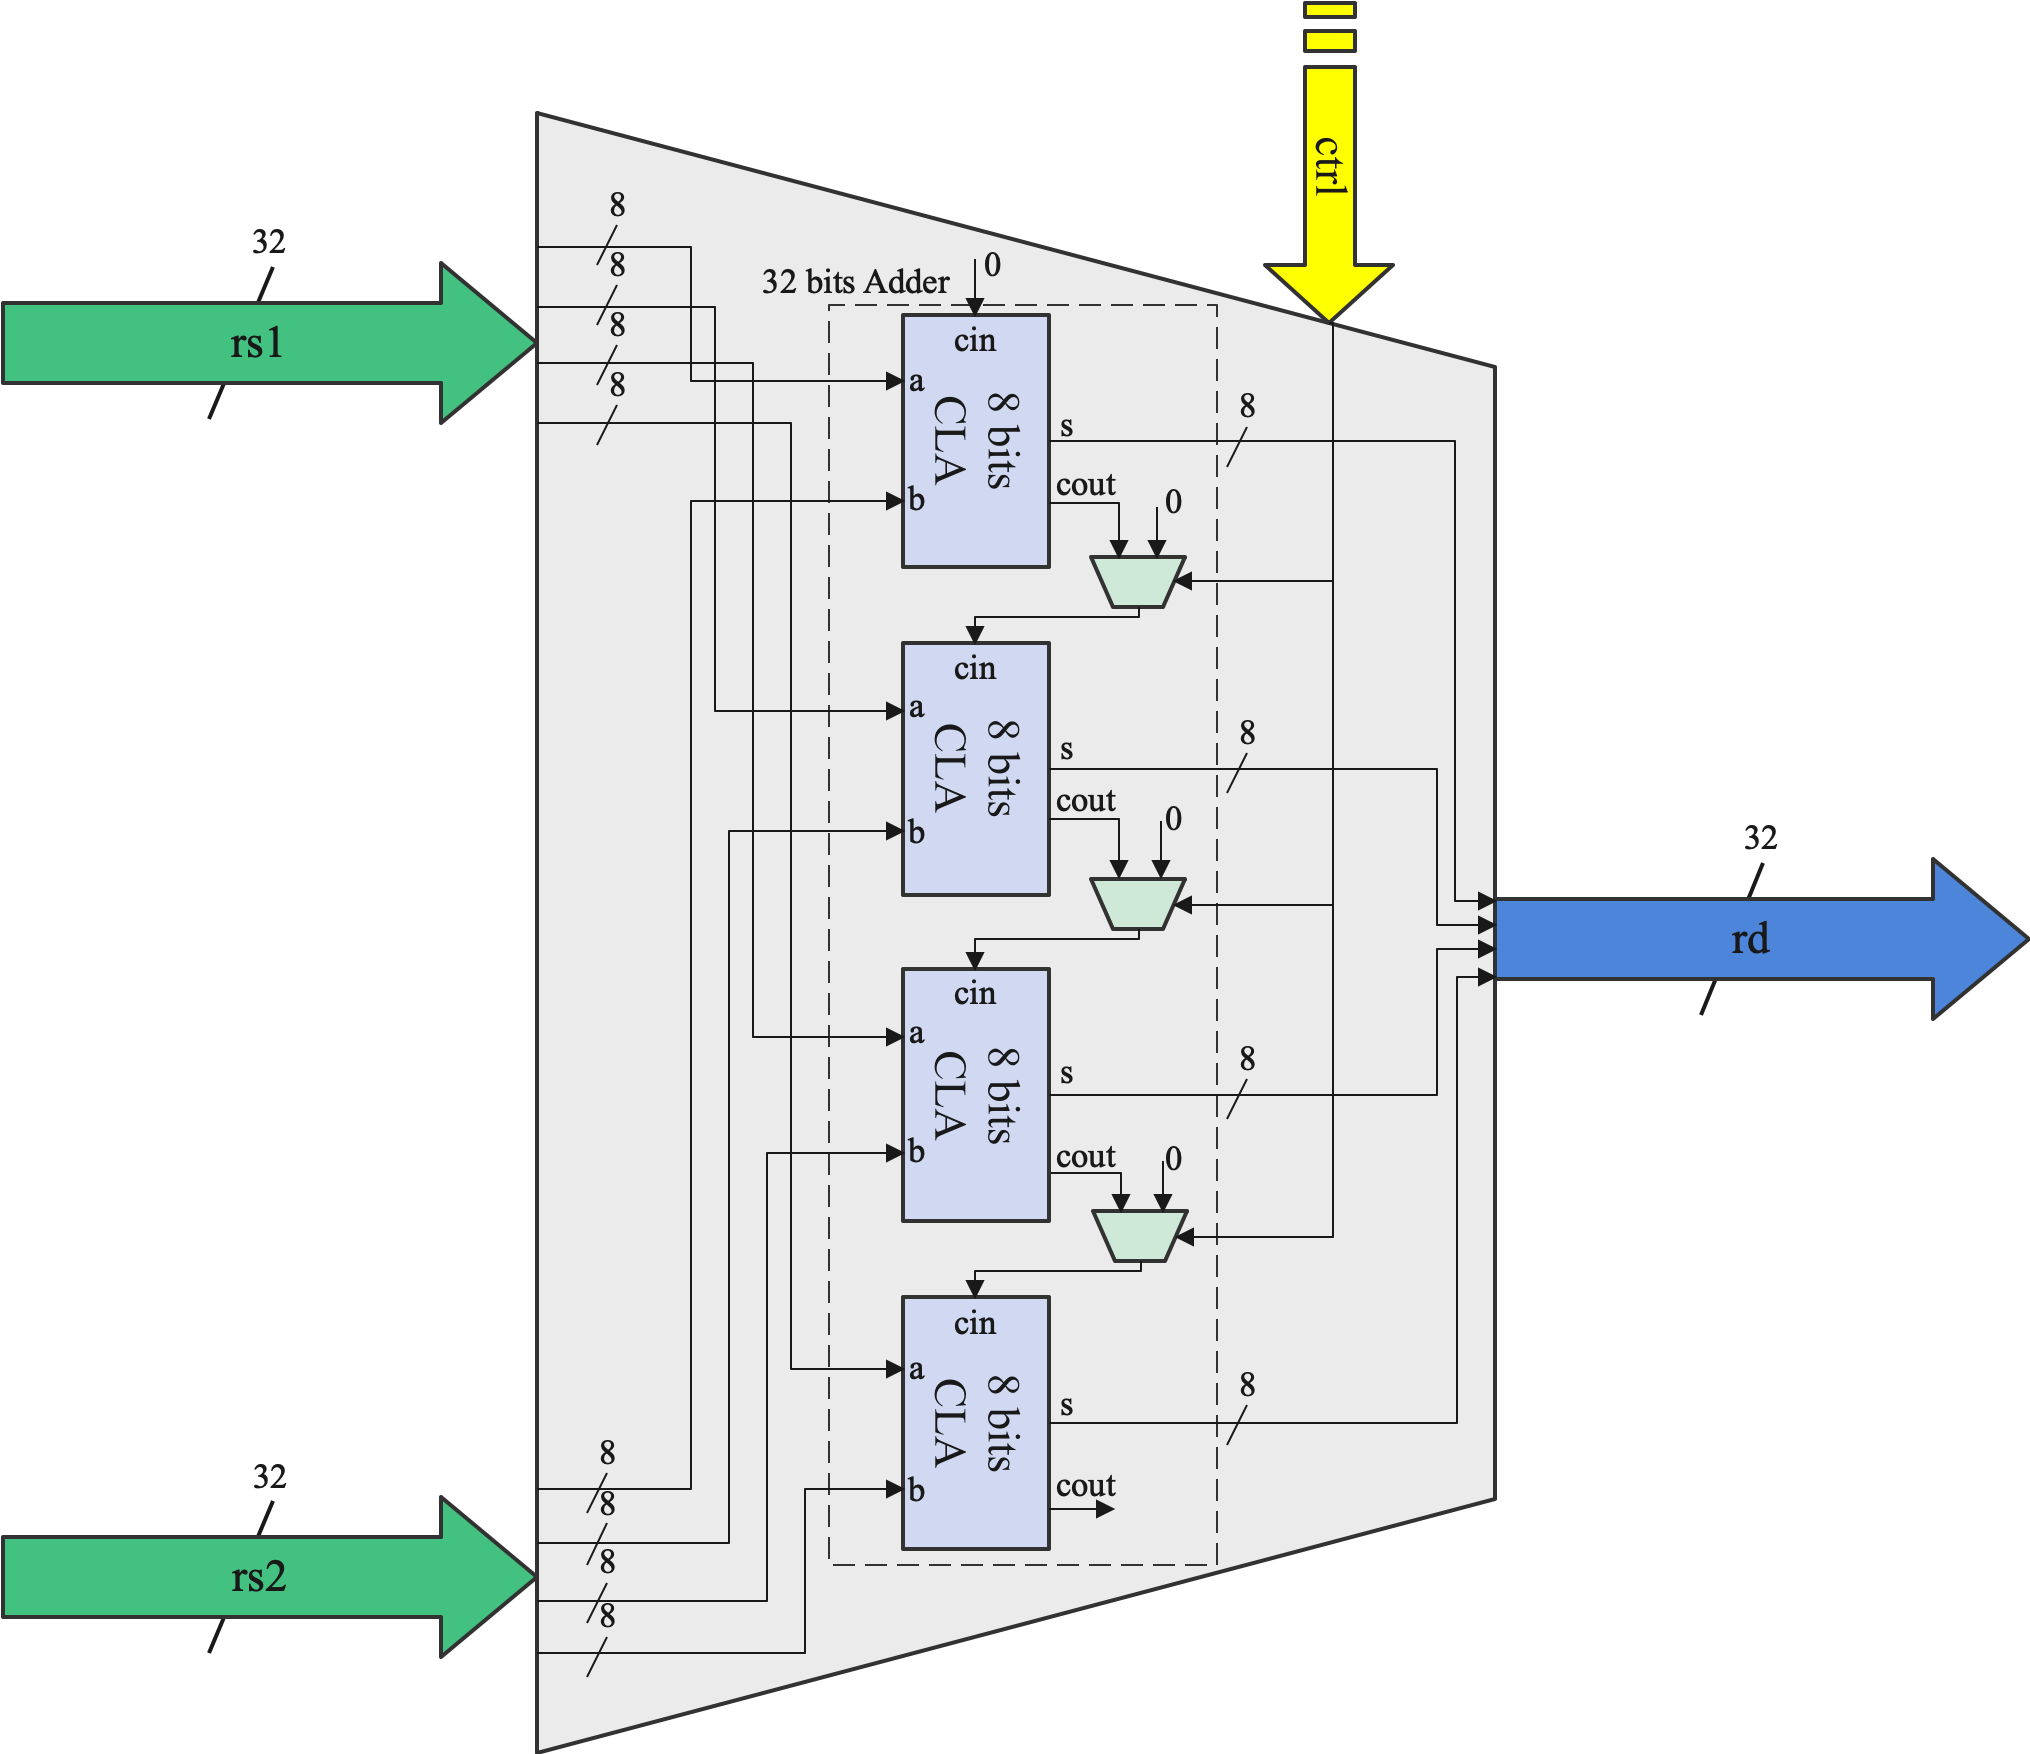
\includegraphics[width=0.95\textwidth]{Photos/ADD8.png}
	\caption{ALU中能够同时执行基本RV32I 32位加减法运算以及“P”扩展指令的SIMD加减运算的32位分区加法器。其中分割为4个8位的先行进位加法器。}
\end{figure}

\section{SoC实现以及相关测试数据}

在本章开头图13给出了包含本文实现的微处理器软核的SoC系统结构概览。SoC使用AMBA AXI4总线来作为内部的高速互联总线,而对于低速的外围设备,如UART、I2C等外设,则使用较为简单的APB总线。AXI4总线与APB总线之间通过APB桥交互。存储器方面,由于SoC进行测试的目标后端为FPGA平台,因此指令以及数据的存储器使用FPGA内置的BRAM资源构成,指令以及数据存储的大小为32K字节。SoC中还包含有一块大小为512字节的Boot ROM,存放启动系统的RISC-V汇编代码。SoC平台同时包含一个支持JTAG的调试器,可以在上位机通过OpenOCD进行GDB调试。调试器、数据及指令存储器通过AXI4总线进行互联。

表4列出了SoC片上系统中存储器以及外设在微处理器中的内存映射地址范围。SoC上电启动后,微处理器的PC启动地址为0x00080000,从Boot ROM中执行相关的配置指令,之后跳转到指令存储器中开始执行程序流。

\begin{table}
	\caption{SoC内存映射地址}
	\centering
	\small 
	\begin{tabular}{ccc}
		\hline 
		用途 & 大小                & 地址范围             \tabularnewline
		\hline 
		指令存储   & 32KB		     & 0x0000 0000 - 0x0000 7FFF \tabularnewline
		Boot ROM   & 512B		     & 0x0008 0000 - 0x0008 01FF \tabularnewline
		数据存储   & 32KB		     & 0x0010 0000 - 0x0010 7FFF \tabularnewline
		外设   & 32KB		     & 0X1A10 0000 - 0X1A10 7FFF \tabularnewline
		调试器   & 4KB		     & 0x1A11 0000 - 0x1A11 0FFF \tabularnewline
		\hline 
	\end{tabular}
\end{table}

其中,32KB的指令存储中0x00000000到0x0000008C地址范围预留为中断向量表,SoC外设使用自定义的16个外部中断与内核交互。

<相关数据>

\section{本章小结}

本章对本文使用PyHCL实现的基于RISC-V的RV32GCP微处理器进行的介绍,对微处理器的流水线、特权级模式以及异常与中断的实现机制、“P”扩展指令集的实现思路以及SoC片上系统进行具体的描述。本文所实现的微处理器在保持低功耗的目标前提下尽可能的考虑性能上的优化,通过使用简单而有效基于4K缓冲区的两位饱和计数分支预测器、紧凑的预取指缓冲区、分区的加法器以及乘法器等设计,以在追求资源与面积最优化的同时,提高微处理器的性能表现。本章的最后给出了包含该微处理器核的SoC片上系统在Xilinx N4 FPGA平台上的各项测试数据。%第三章
	\chapter{PyHCL验证方法概述}

本章对PyHCL所包含的验证方法进行概述,包括基本单元测试使用的PyHCL-Tester、基于UVM的大规模集成测试框架PyUVM、以及在此基础上的针对RISC-V微处理器的差分测试框架。PyHCL所设计的验证方法是为了达到如下的目标:

\begin{enumerate}
	\item 填补其他硬件生成框架所缺乏的验证工具或方法。开发者可以通过PyHCL完成电路设计以及验证的全部过程,而不需要切换到其他的验证工具流或者语言。不包含有验证工具或方法的硬件生成框架存在一个难以解决的难题,那就是设计得到的代码要进行验证,则必须生成Verilog代码。常见的验证工具流仅支持Verilog或SystemVerilog代码的输入,而当基于高层次的电路表述编译为Verilog后,则通常会损失原设计中的信息,导致验证过程举步维艰。
	\item PyHCL的验证方法涵盖了各级别验证的粒度以及策略。在验证粒度方面,PyHCL涵盖了以单个模块为基准的单元测试到基于SoC片上系统的大规模集成测试。在验证策略方面,PyHCL支持白盒、黑盒以及灰盒测试。
	\item 支持UVM验证方法学。PyHCL包含基于Python而非SystemVerilog的大规模UVM验证平台PyUVM,支持验证复用以及随机向量测试的特性,同时也是实现本文微处理器的差分测试框架的基础。
\end{enumerate}

本章将介绍PyHCL验证方法中包括的主要模块:基于模块单元测试PyHCL-Tester、大规模集成测试框架PyUVM、针对第三章中实现的微处理器的差分测试框架。本章的最后将会给出各个PyHCL验证工具与当前流行的开源验证框架的性能对比。

\section{PyHCL-Tester与PyUVM}

PyHCL-Tester是PyHCL提供的基于模块单元测试的轻量级验证工具,PyHCL-Tester的内核基于开源的验证引擎Verilator[50],Verilator可以提供在开源验证工具当中最快的仿真速度。与基于Verilog Testbench的单元测试方法不同,PyHCL-Tester通过将Python仿真脚本内嵌在PyHCL电路RTL设计代码中实现,因此PyHCL-Tester可以给使用者带来快速的模块级的黑盒验证测试策略。相对于一些其他的基于Python的硬件生成框架,某些HGF会使用基于Python的仿真引擎来作为框架使用的验证工具,但是囿于Python固有的解释器解释执行而导致其性能较为平庸。 因此,PyHCL-Tester选择采用目前开源仿真引擎中最快的Verilator来作为内核,而Python-Tester则作为仿真的前端,通过管道的方式将仿真的数据以及指令通过自定义的协议发送给Verilator后端,并将Verilator后端的仿真结果再通过管道接收。图4-1展示了PyHCL-Tester以及结合FIRRTL执行器Treadle[51]的验证测试框架图。

\begin{figure}[htbp]
	\centering
	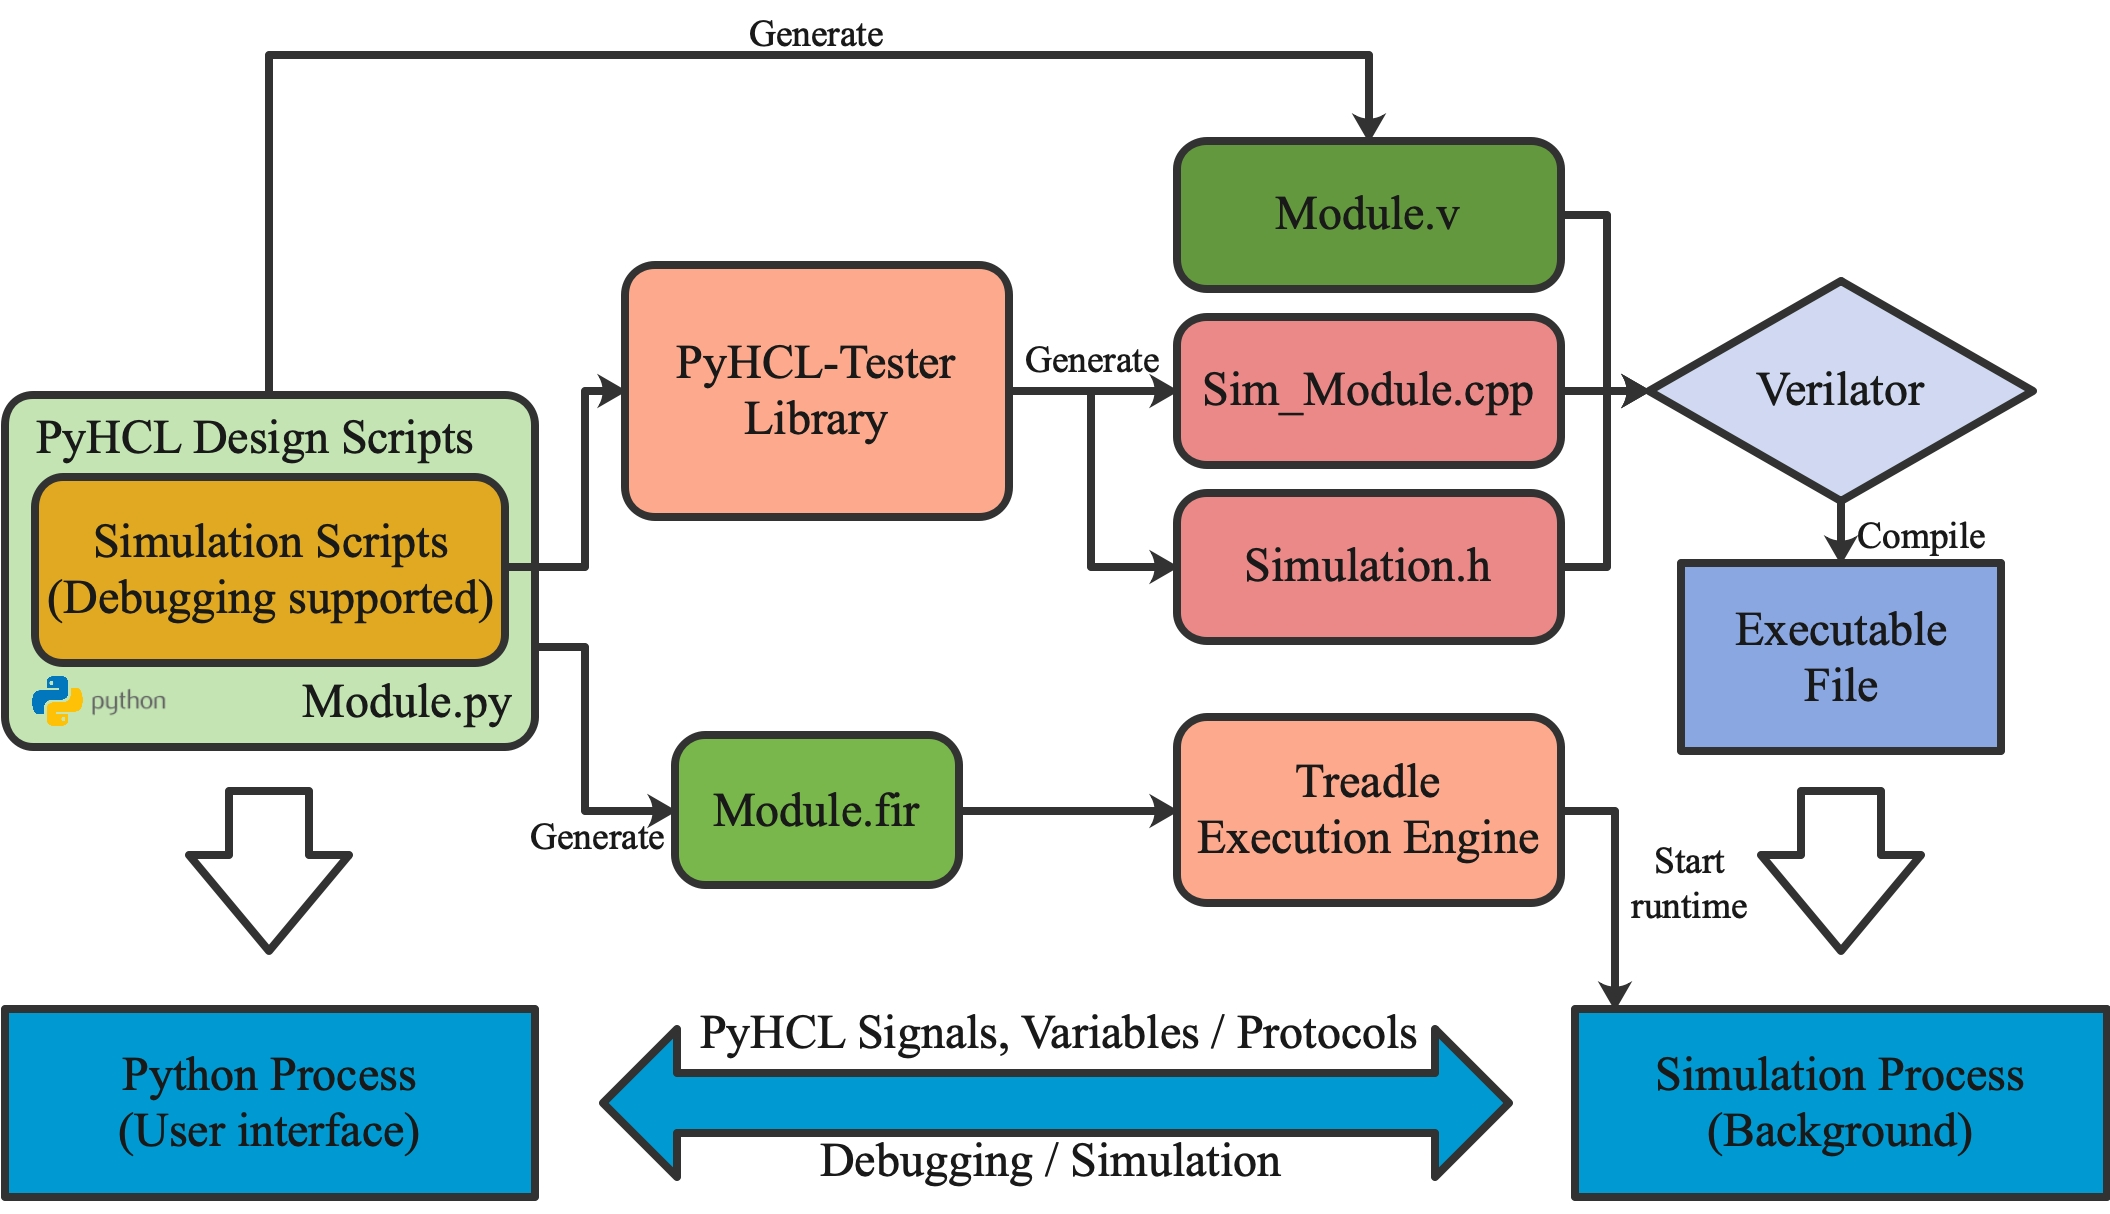
\includegraphics[width=0.95\textwidth]{Photos/PyHCL-Tester.jpg}
	\caption{PyHCL-Tester及Treadle的验证测试框架图}
\end{figure}

PyHCL-Tester库包含有生成C/C++仿真头文件所需要的基础模版,并提供若干个用户接口函数允许使用者基于2.1节中提供的PyHCL原语编写仿真脚本。举例来说,PyHCL-Tester中提供两个主要的接口来操纵所需要仿真的模块的IO端口:poke()用于提供给模块输入端口以激励,而peek()用于监测模块输出端口再各个时钟周期的输出信号变化,并通过该接口在仿真过程中实时返回给PyHCL-Tester前端。与传统的使用Verilog进行Testbench单元测试的方法不同,使用Verilog编写Testbench在对待测模块(Design Under Test,DUT)的单元测试代码时,激励的生成需要经过繁杂的时钟定义/生成、激励定义与描述的过程。而在PyHCL-Tester中,对输入端口的激励以及输出端口的监测可以直接指定模块对应的PyHCL原语,且激励信号的值也可以直接使用Python内置数据类型,且对于较为复杂的激励信号也可以使用第三方的Python科学计算库来生成。PyHCL-Tester的仿真脚本内嵌到PyHCL电路设计代码中,当仿真开始后,PyHCL电路设计部分的代码通过PyHCL及FIRRTL编译器生成Verilog代码,而内嵌在其中的PyHCL-Tester仿真脚本则生成作为Verilator输入的C/C++仿真头文件,这其中包含有预定义的管道以及通信协议结构代码。在这之后,电路RTL设计代码(Verilog)以及C/C++仿真头文件作为Verilator的输入进行编译,Verilator将Verilog描述的RTL级电路编译成等效的并发C/C++模型,最终生成对应的后台仿真可执行文件。当用户启动仿真时,前端的PyHCL-Tester仿真脚本进程调用后台生成的可执行文件作为后台仿真进程,两个进程之间通过管道以及预定义好的协议进行通信,协议主要定义了后端仿真进程的控制信号,如时钟周期步进、仿真启停等,前端PyHCL-Tester仿真脚本进程提供输入信号激励传递到后台C/C++仿真进程,时钟周期步进后,后台C/C++仿真进程返回模块输出端口信号的值到前端PyHCL-Tester仿真脚本。对于使用者来说,信号激励的输入与输出返回都是基于Python内置数据类型的,而不需要了解内在的仿真机理。因此,通过这种将电路设计以及仿真验证放在同一个接口层次的设计模式,PyHCL-Tester可以快速进行单个模块的单元验证测试,同时,PyHCL-Tester在性能方面与Verilator基本持平。

PyHCL-Tester也存在一定的缺点,虽然PyHCL-Tester在仿真性能上非常突出,但是对于大规模的系统级测试需要耗费大量额外的时间来编译仿真环境,因此PyHCL-Tester仅适合在小规模的单元测试中使用。此外,PyHCL-Tester使用黑盒的验证策略,因为PyHCL-Tester仅支持对模块的输入输出端口进行交互,而模块内部的信号情况是未知的。当测试出现错误时,是无法精确定位具体的电路逻辑的。为了解决该问题,PyHCL提供了一种辅助手段支持单元测试:Treadle。Treadle是一个FIRRTL的执行器,可以直接读取FIRRTL级的电路设计,并在仿真运行时返回内部所有信号如寄存器、线网的当前值。当前设计出现问题时,可以将后端的C/C++仿真进程切换到Treadle,并直接执行对应PyHCL电路RTL代码所生成的FIRRTL代码。用户使用相同的接口函数来为Treadle提供输入信号激励,并获取输出信号的值。与Verilator不同,使用Treadle可以在各个周期获取到模块内部信号的值,这种方式类似于调试中的断点,可以精确定位到出现问题的时钟周期以及模块内部具体的寄存器或者线网。Treadle所提供的验证策略属于白盒验证策略,DUT模块在仿真过程中会暴露所有内部信号的值。虽然Treadle可以提供相当详细的运行时信息,但是其缺点在于仿真的性能较差。因此使用PyHCL进行单元测试过程中,明智的做法是结合PyHCL-Tester以及Treadle使用。

PyHCL提供PyHCL-Tester作为单元测试以及小规模的功能测试使用。而对于大规模的系统级验证测试或SoC平台的集成测试,验证测试环境更需要考虑可重用性的问题。模块级的单元测试需要监测验证模块所有输入输出端口的值与参考模型的行为是否一致,而系统级的测试则专注于在实际的应用场景中系统中各个不同模块之间的交互。UVM验证方法学广泛应用在系统级的验证当中,其主要的验证思路是验证环境重用以及随机测试。但绝大多数的硬件生成框架都不支持基于UVM的验证环境,基于这些硬件生成框架的电路设计在需要进行大规模UVM验证时,都需要基于SystemVerilog重新搭建UVM测试平台,这将会导致设计与验证之间完全分隔开来,不利于硬件敏捷设计方法的应用。为了解决这一问题,PyHCL引入了支持UVM验证方法学的验证平台PyUVM。

PyUVM主要基于协程的开源协同仿真测试环境cocotb[52]搭建,cocotb允许使用者通过Python搭建基于UVM的验证测试环境。使用Python而非SystemVerilog来搭建UVM验证测试环境具有许多优势,如在Python中定义UVM测试中所需要使用的参考模型相比于使用SystemVerilog来说要相对简便很多。参考模型用于模拟实现相关算法的电路行为,UVM验证环境通过比对电路仿真验证以及参考模型的结果来验证DUT的设计是否符合规范。SystemVerilog一般需要导入外部的C/C++算法模型作为参考模型使用,而在PyUVM中则可以直接使用Python来对参考模型进行建模。此外,由于Python自身的解释执行特性,所有在PyUVM中的Python测试协程都可以在验证过程中随时修改并重启,而不需要重新编译耗费大量的时间,而Verilator则在对仿真头文件发生更改后,都需要重新进行编译。

基于cocotb的PyUVM的测试协程通过函数装饰器实现,cocotb包含一个对协程的调度器来调度不同测试协程的运行。与其他基于SystemVerilog的UVM验证框架不同,PyUVM不需要编写额外的RTL级验证代码。PyUVM同时支持多种后端的仿真引擎,包括Verilator、Icarus Verilog[53]、ModelSim等等。然而,PyUVM也存在一定的缺点,它使用VPI(Verilog Procedural Interface)作为Python构建的UVM验证测试环境与仿真器的交互接口,会带来一定的额外性能损耗。表4-1对PyHCL所提供的三种验证方法及工具进行了总结与对比。

\begin{table}
	\caption{PyHCL提供的三种验证方法及工具的对比}
	\centering
	\small 
	\begin{tabular}{cccc}
		\hline 
		特性 & PyHCL-Tester                & Treadle & PyUVM            \tabularnewline
		\hline 
		验证粒度级别   & 模块级		     & 模块级   & 系统级 \tabularnewline
		验证策略   & 黑盒		     & 白盒   & 黑盒 \tabularnewline
		可重用性   & 低		     & 低   & 很高 \tabularnewline
		仿真性能   & 高		     & 很低   & 中等 \tabularnewline
		参考模型复杂度   & 低		     & 无   & 高 \tabularnewline
		定位设计错误的难度   & 高		     & 很低   & 高 \tabularnewline
		开发验证环境所需的工作量   & 低		     & 低   & 高 \tabularnewline
		\hline 
	\end{tabular}
\end{table}

\section{基于多级验证环境的差分测试框架}

本小节介绍结合PyHCL所提供的三种验证测试方法所搭建的针对本文所实现微处理器的多级验证差分测试框架与环境。在4.1节中提到,PyHCL提供了三种不同的验证测试方法,从表5中可以发现,每种方法都有各自的利弊。为了充分发挥每种验证测试方法的优点,本文搭建了结合上述三种验证测试方法的多级验证测试环境,并在其中实现了一个针对第三章中实现的RV32GCP处理器的差分测试框架。该多级验证测试环境涵盖所有的验证粒度级别以及验证策略,包括灰盒验证策略。灰盒验证策略允许用户在保证仿真性能以及验证可重用性的同时,还可以快速定位到设计逻辑中的错误。该多级验证环境还可以轻松地与PyHCL实现的电路设计交互,这是因为4.1节中提到的PyHCL提供的三种验证方法都具有通用的接口,可以直接加载PyHCL设计并操作设计中的PyHCL电路实体原语。此外,该多级验证环境还可以通过Python导入外部的包或工具。同时,该多级验证环境通过若干通用可配置的模块组成,这些模块可以在整个设计和验证过程中重用,而不需要任何重大的修改,这种设计模式可以显著缩短开发周期。

图4-2给出了基于该多级验证环境的差分测试框架结构图。该多级验证环境基于cocotb来进行构建,这是因为cocotb带有原生的Python UVM验证方法支持。该多级验证环境可以分割成四个主要模块:使用PyHCL描述的待验证电路(DUT)、参考模型、仿真引擎以及前端的Python接口。在针对本文实现微处理器的差分测试框架中,DUT是RV32GCP的微处理器内核。参考模型是主流的RISC-V模拟器QEMU[54]或NEMU[55]。差分测试的主要思想就是对于根据同一种规范的两种实现,给定相同的有定义的输入,它们产生的行为应该一种。对于本差分测试框架,两种实现指的就是本文实现的RV32GCP微处理器软核以及RISC-V模拟器QEMU或NEMU。NEMU是QEMU的简化版本,两者的主要目的是使用C/C++代码来模拟一个单核或多核RISC-V处理器的行为。多级验证测试环境中实现了两种混合的验证测试方法:PyHCL-Tester+Treadle以及PyHCL-Tester+PyUVM,前者应用在模块级的单元测试当中,后者应用在系统级的大规模差分测试当中。其中PyHCL-Tester+PyUVM的方法使用默认的Icarus Verilolg仿真引擎,前端的Python接口用于与使用者进行交互。

\begin{figure}[htbp]
	\centering
	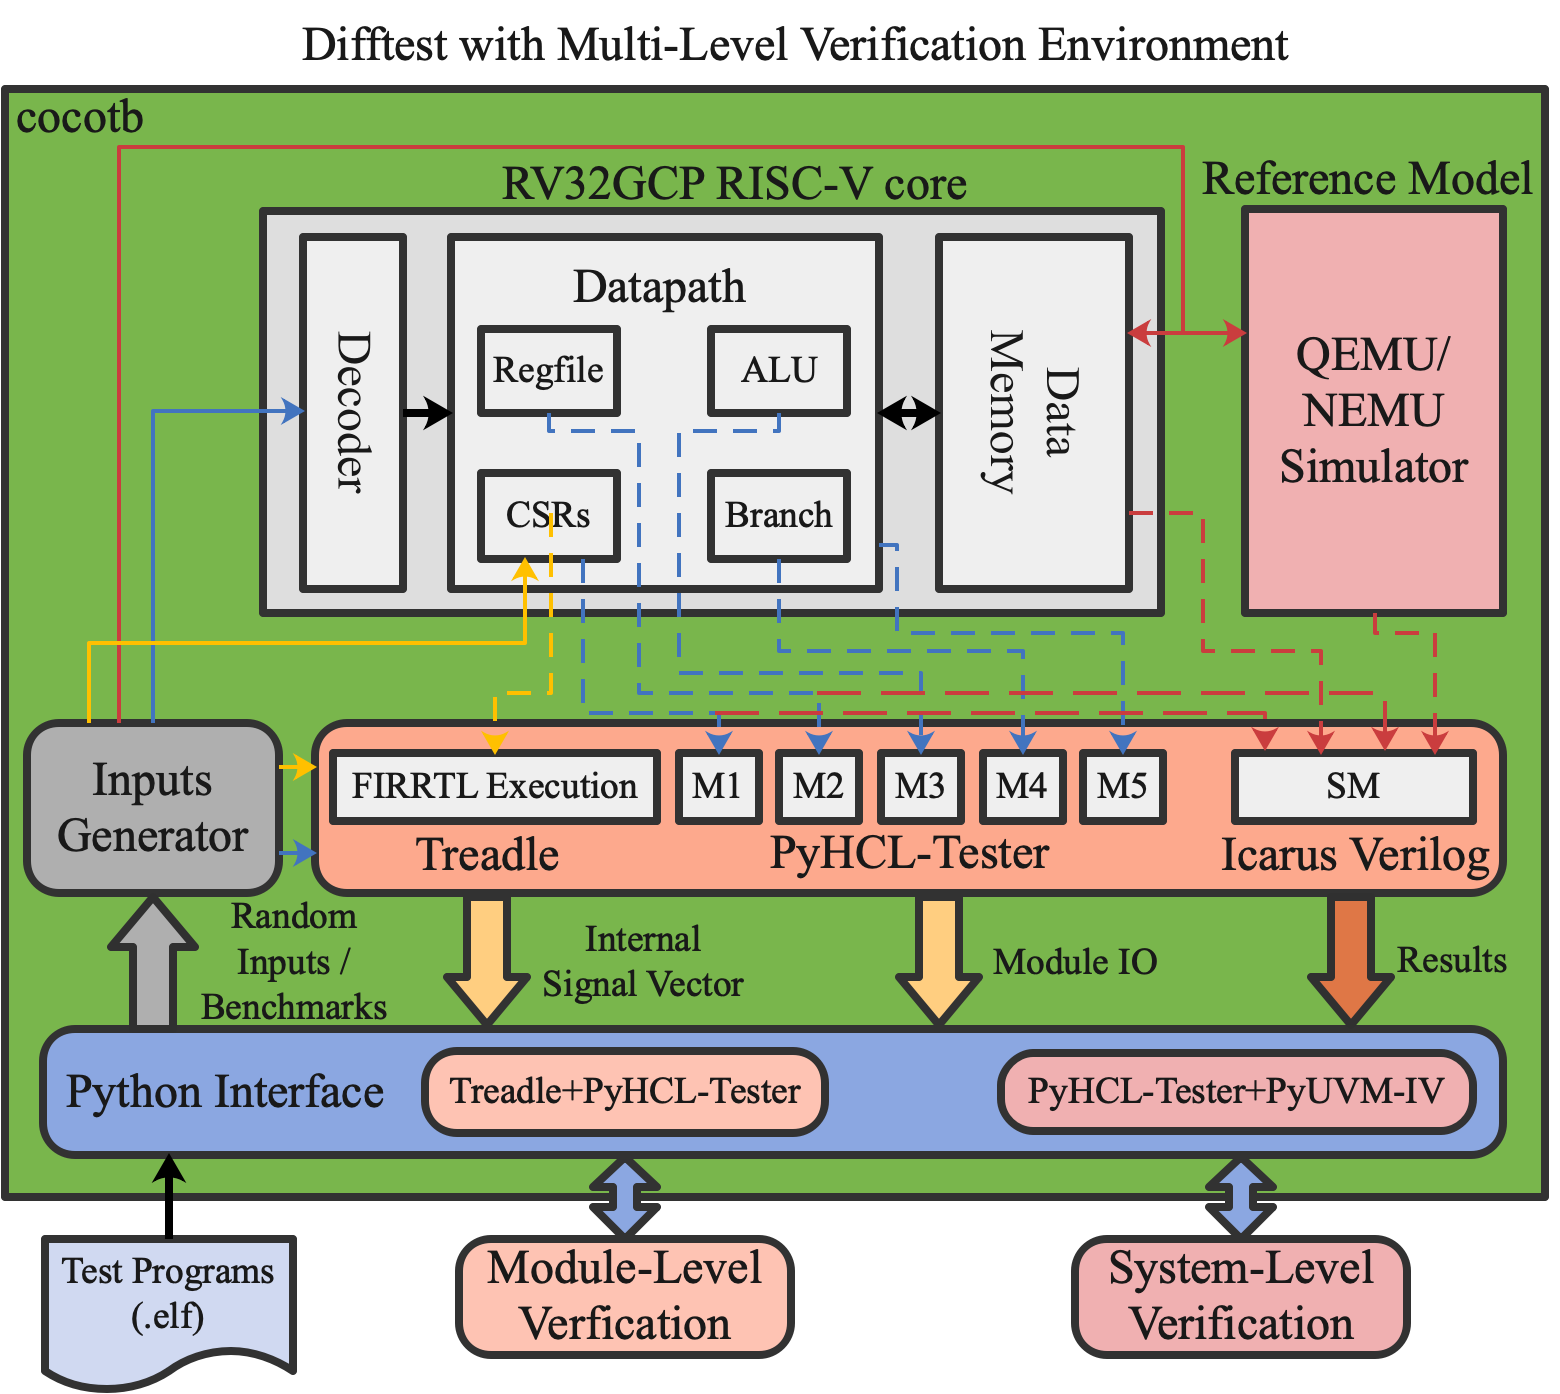
\includegraphics[width=0.95\textwidth]{Photos/multi-level-ve.png}
	\caption{基于多级验证环境的差分测试框架结构图}
\end{figure}

当使用该多级验证环境对本文所实现的RV32GCP微处理器进行验证时,首先从验证粒度较小的模块级单元测试开始。举例来说,当验证控制状态寄存器组CSRs单个模块时,多级验证环境使用PyHCL-Tester混合Treadle的验证方法。在图20当中使用黄色以及蓝色的箭头来分别表示Treadle以及PyHCL-Tester的数据流,实线代表输入数据,虚线代表输出数据。为了达到单个模块灰盒测试的目的,该方法使用PyHCL-Tester来监控模块的输出,与此同时在执行设计生成的FIRRTL代码的Treadle中插入若干断言。当Treadle执行到这些断言时,就会触发断点并返回当前模块内部信号值组成的向量。为了测试CSRs设计的正确性以及鲁棒性,多级验证环境会提供大量自定义或者随机生成的输入信号,并同时作为PyHCL-Tester以及Treadle的输入激励。此时用户可以通过PyHCL-Tester中对模块输出信号的监控单元来与模块级参考模型进行对比,来查看设计是否出错。需要注意的是,模块级的参考模型需要用户自定义,而非通过QEMU或NEMU,后者仅使用在大规模的差分测试当中。在图7中,这些监控单元使用MX来表示。如果模块的输出发现问题,用户可以随时切换到Treadle执行器,执行出现问题前后的若干时钟周期的的一小段仿真过程,根据断言返回的内部信号向量来定位PyHCL电路逻辑设计中产生的问题。Treadle在执行短周期仿真的性能与PyHCL-Tester并没有太大的区别。这种方法的关键点在于,结合PyHCL-Tester仿真的高性能以及Treadle定位设计错误的简便性,来达到在模块级单元测试中的灰盒验证目的。这种思路可以扩展到子系统级的功能验证,如针对条件分支的功能验证。在这种情况下,我们可以预先定义若干个包含条件分支的RISC-V汇编代码片段来作为译码器的输入,并使用PyHCL-Tester来观察若干模块的输出信号。如果输出信号发生错误,则首先根据不同的监控单元定位出错的模块。当问题模块被定为后,则可以切换到模块级单元测试的验证方法PyHCL-Tester+Treadle,来定位模块内部PyHCL电路逻辑设计中的错误。

当微处理器内核原型系统设计完成后,微处理器内核中的子模块都已经通过单元测试。此时多级验证平台将对整个微处理器核进行大规模的系统级测试。系统级的验证测试主要使用差分测试框架来完成,差分测试的实现主要通过将相同的RISC-V测试代码片段同时作为RV32GCP以及QEMU/NEMU模拟器的输入,在执行后,通过比对模拟器以及微处理器软核的处理器架构状态来查看微处理器是否存在逻辑错误。微处理器架构状态包括通用寄存器组、状态控制寄存器组CSRs、数据存储。作为输入的RISC-V测试代码可以使用随机指令生成框架如riscv-torture[56]或者是预定义的RISC-V标准测试例程如riscv-tests。测试代码通过Python接口导入到RV32GCP内核以及QEMU/NEMU模拟器的指令存储器当中。在测试代码的执行过程中,PyUVM的模拟器监控单元SM在每个时钟周期会实时比对微处理器内核与模拟器通用寄存器组的值,当出现差异时就会立刻抛出异常,并返回当前出错的指令以及时钟周期。对于riscv-tests,在测试代码执行完成后,还会检查存储器特定地址区域之间的差异,这是因为riscv-tests通过在数据存储特定地址写入若干标记,在测试例程结束后通过检查存储区目标地址微处理器是否存在与模拟器相同的标记即可判断测试是否通过。该基于Python的差分测试框架相对于基于SystemVerilog实现的差分测试框架性能要更好,这是因为SystemVerilog实现的差分测试框架,在编译后都会变成事件和队列的模型,并以事件驱动的方式来运行,因此本多级验证环境中基于Python实现的差分测试框架可以在测试运行时同时对比通用寄存器组值并即时抛出异常,而不会造成错误继续传播,造成调试的困难。

差分测试框架不单止使用了基于PyUVM的Icarus Verilog引擎进行验证测试,在本多级验证环境中还结合了PyHCL-Tester辅助测试代码的验证过程。当测试代码验证过程中抛出异常后,若发现错误来自于某特定的模块,则需要PyHCL-Tester介入。如果对单个模块使用PyUVM来重新执行测试代码,如4.1节中提到了,基于cocotb的PyUVM由于使用了VPI接口,在执行单模块的大量指令测试时会产生大量的额外开销。由于在单元测试中已经使用了PyHCL-Tester对各模块构建并编译了对应的监控单元,因此在大规模集成验证测试中可以重用这些已经编译好的C/C++仿真头文件,来监控测试代码执行过程中在异常指令附近该模块的输出信号是否有异常。PyUVM+PyHCL-Tester的方式可以作为大规模验证测试的灰盒验证策略,PyUVM可以快速构建差分测试平台并进行实时通用寄存器组的检查与对比,但无法得知具体模块的信号输出情况,而PyHCL-Tester可以提供该信息,以在保持性能的情况下得知微处理器内核内部的信号情况。

本节所实现的多级验证测试环境在对LeNet-5[57]以及VTA[58]等加速器软核实现中亦进行相关的验证测试,以确保该验证环境在异构系统中的适用性。本节所实现的多级验证测试环境的结果将在4.3节中给出。此外,本节中所实现的多级验证测试环境也是组成本文微处理器开发流程中的重要组成部分,可以加速对RV32GCP微处理器的验证过程,从而缩短每个功能的迭代开发流程,在第五章将会给出对本文所实现微处理器的硬件敏捷开发模型。

\section{PyHCL验证工具性能对比}

本节将对PyHCL中所提供的验证工具以及方法进行性能对比。表4-2给出了除本文实现的微处理器外到目前为止使用PyHCL实现的其他电路结构在Xilinx Artix 7 XC7A200T FPGA开发版上的综合情况,该开发版包含有215360个LUT,269200个可配置的触发器,740个DSP单元以及13150kb大小的BRAM。

\begin{table}
	\caption{使用PyHCL的电路RTL实现在Artix 7 FPGA开发板上的资源占用情况以及最大时钟频率}
	\centering
	\begin{tabular}{cccccc}
		\toprule
		\multirow{2}[2]{*}{设计} & \multicolumn{4}{c}{硬件资源使用} & \multicolumn{1}{c}{\multirow{2}[2]{*}{最大时钟频率 (MHz)}} \\
		\cmidrule{2-5}          & LUTs  & FFs   & DSPs  & \multicolumn{1}{c}{BRAM (bits)} &  \\
		\midrule
		RV32I Pipeline & 1004  & 441   & -     & 32K   & 141 \\
		LeNet-5 Accelerator & 18341 & 6877  & 144   & 768K  & 148 \\
		PicoRV32 & 879   & 578   & -     & 32K   & 243 \\
		VTA   & 40879 & 8689  & 114   & 3648K & 79 \\
		AXI4-Full & 191   & 224   & -     & -     & 294 \\
		Wallace Tree Multiplier & 50    & -     & -     & -     & 400 \\
		\bottomrule
	\end{tabular}%
\end{table}%

RV32IMC流水线是一个极小型的实验性RISC-V内核实现,是本文实现的RV32GCP微处理器的前身。PicoRV32是在第1.1.2节中提到的面向FPGA面积优化的RISC-V内核实现。LeNet-5加速器是对经典手写数字分类识别神经网络LeNet-5的硬件加速实。VTA是一个可编程的加速器架构,是TVM[59]架构的硬件扩展之一,可以借助TVM的上层工具链,构成端到端的深度学习加速器解决方案。PicoRV32以及VTA为使用PyHCL重构后综合得到的结果。AXI4是对AMBA AXI4主从端的逻辑实现。在最后还给出了使用PyHCL实现的基于华莱士树的乘法器综合结果。

表4-3给出了PyUVM中提供的三种验证方法及工具与Verilator仿真验证的性能的对比,其中PyUVM使用默认的Icarus Verilog仿真引擎。仿真验证测试的电路软核设计与表4-2相同。测试中使用的Verilator版本为4.034,Icarus Verilog版本为10.3,cocotb版本为1.3.2。每种方法测试数据通过10次重复测试取平均值得到,每次测试仿真执行10万个时钟周期。

\begin{table}
	\caption{PyHCL验证测试工具性能 (单位:秒)}
	\centering
	\begin{tabular}{ccccc}
		\toprule
		\multicolumn{1}{c}{设计} & PyHCL-Tester& PyUVM - Icarus Verilog & Treadle & Verilator \\
		\midrule
		RV32IMC流水线 & 0.78  & 15.81  & 29.36  & 0.79  \\
		LeNet-5加速器 & 5.70  & 28.64  & 175.74  & 5.60  \\
		PicoRV32 & 0.12  & 12.97  & 8.16  & 0.13  \\
		VTA   & 6.29  & 35.03  & 296.16  & 6.17  \\
		AXI4主从端 & 0.08  & 12.85  & 4.60  & 0.09  \\
		华莱士树乘法器 & 0.06  & 12.04  & 1.12  & 0.07  \\
		\bottomrule
	\end{tabular}%
\end{table}%

从表4-3中,可以发现PyHCL-Tester的性能与Verilator接近,这是因为两者都是以轻量级高速仿真为目标的仿真器。然而,两者都有相同的缺点:PyHCL-Tester以及Verilator都不支持模块内部信号的监控。而Treadle可以在运行时保存模块内部所有信号的值,因此可以随时获取模块内部信号在当前周期的值,然而代价是相对较差的性能。在相同条件下,Treadle相比PyHCL-Tester的仿真时间平均要慢38倍,最慢要达到67倍。但同时也要注意到在小模块的仿真,如华莱士乘法树当中,Treadle的仿真时间还处于可以接受的范围内。对于PyUVM,在验证测试时通常使用默认的Icarus Verilog仿真引擎,因为其比Verilator要更稳定。可以发现,PyUVM的仿真性能介于PyHCL-Tester以及Treadle之间,且具有最为稳定的仿真验证性能表现:对于PyHCL-Tester以及Treadle,最长仿真时间与最短仿真时间的比值为105以及264。然而对于使用Icarus Verilog的PyUVM,最长仿真时间与最短仿真时间的比值约为3。

从表4-3可以得出,PyHCL所提供的所有单个验证方法或工具应用在每种验证场景中都有一定的尴尬之处。对于PyHCL-Tester来说,其具有最佳的仿真验证性能,但无法获取模块内部的信号值信息。同时,PyHCL-Tester相比PyUVM在大规模的集成测试中需要耗费大量时间编译验证环境,此外,PyHCL-Tester还不具有验证环境的重用性。对于Treadle来说,它在运行时保存有模块所有内部信号的信息,但因此需要承受较低仿真性能的代价。对于PyUVM来说,通过使用Icarus Verilog仿真引擎可以达到最为稳定的仿真性能表现,但是在小模块的仿真时会带来额外的性能损耗。为了解决上述问题,在4.2节中多级验证测试环境中所提出的两种混合的仿真测试方法:PyHCL-Tester+Treadle以及PyUVM+PyHCL-Tester,两者分别应用在模块级单元测试以及大规模的集成测试中。表4-4给出该多级仿真验证环境中所有验证方法的性能,包括3种单个验证方法以及2个混合的验证方法。对于模块级的单元测试,本文从RV32GCP的微处理器核中提取CSRs以及ALU两个模块以及VTA的取指单元进行测试。对于大规模的系统级测试,本文选用RV32IMC的流水线、LeNet-5以及VTA加速器进行测试。

对于模块级的单元测试,PyHCL-Tester+Treadle的性能要显著优于Treadle,带来平均63\%的性能提升,且仿真的时间也平均只比PyHCL-Tester要慢9倍左右,对于单模块的测试上来说,基本上都在1s的时间浮动,这对于模块级的单元测试来说是可以接受的。与此同时,使用该方法还可以在仿真同时获取模块内部的信号值信息。对于大规模的系统级验证测试,PyUVM+PyHCL-Tester的性能要比PyUVM带来平均40\%的性能提升。PyUVM+PyHCL-Tester的性能虽然逊于PyHCL-Tester,但在大型电路设计项目上,如VTA以及LeNet-5上两者的性能差距要更小。对于大规模项目来说,这种差距也是可接受的。此外,PyUVM+PyHCL-Tester在大规模系统级验证测试上的稳定性要优于PyHCL-Tester,前者最长仿真时间与最短仿真时间的比值为1.7,而后者则达到8。

\begin{table}
	\centering
	\caption{多级验证环境的仿真性能(单位:秒)}
	\begin{tabular}{ccccccc}
		\toprule
		验证粒度级别 & 设计 & Py-T & TDL & PyUVM-IV & PT+TDL & PU-IV+PT\\
		\midrule
		\multirow{3}[1]{*}{模块级} & RV32IMC CSRs & 0.14  & 4.53  & -     & \textbf{0.59 } & - \\
		& RV32IMC ALU & 0.06  & 0.87  & -     & \textbf{0.42 } & - \\
		& VTA 取指单元 & 0.09  & 3.51  & -     & \textbf{1.79 } & - \\
		\midrule
		\multirow{3}[1]{*}{系统级} & RV32IMC流水线 & 0.81  & -     & 18.53  & -     & \textbf{10.96 } \\
		& LeNet-5加速器 & 5.67  & -     & 27.07  & -     & \textbf{17.26 } \\
		& VTA   & 6.30  & -     & 33.63  & -     & \textbf{18.80 } \\
		\bottomrule
	\end{tabular}%

\begin{threeparttable}
	\begin{tablenotes}
		\linespread{1.4}
		\footnotesize
		\item Py-T = PyHCL-Tester
		\item TDL = Treadle
		\item PyUVM-IV = PyUVM with Icarus Verilog
		\item PT+TDL = PyHCL-Tester + Treadle
		\item PU-IV+PT = PyUVM with Icarus Verilog + PyHCL-Tester
	\end{tablenotes}
\end{threeparttable}
\end{table}%

\begin{table}
	\caption{不同验证方法构建验证环境时间的对比(单位:秒)}
	\centering
	\begin{tabular}{cccc}
		\toprule
		设计 & PyHCL-Tester & PU-IV+PT* & PyUVM-IV \\
		\midrule
		RV32I Pipeline & 3.66  & 0.62 & 0.67  \\
		LeNet-5 Accelerator & 6.05  & 3.16 & 3.07  \\
		VTA   & 8.87  & 2.80 & 2.64  \\
		\bottomrule
	\end{tabular}%
	
	\begin{threeparttable}
		\begin{tablenotes}
			\linespread{1.4}
			\footnotesize
			\item[*] PyUVM with Icarus Verilog + PyHCL-Tester
		\end{tablenotes}
	\end{threeparttable}
\end{table}%

表4-5给出了PyHCL-Tester、PyUVM以及PyUVM+PyHCL-Tester的验证环境构建时间比较。测试的环境配置与仿真环境相同。可以发现,混合的PyUVM+PyHCL-Tester的构建时间比PyHCL-Tester要更快,而与PyUVM比较接近。PyUVM+PyHCL-Tester的构建时间平均比PyHCL-Tester要快66\%。除此之外,在验证环境发生改变时,PyHCL-Tester需要重新编译整个验证环境,而PyUVM+PyHCL-Tester则只需要动态编译改变的部分。

综上所述,本章中提出的两种混合的验证测试策略结合了单个不同验证方法的优势并保持了相对较高的仿真性能。对于模块级的单元测试,PyHCL-Tester+Treadle的混合策略可以在保持高仿真性能的同时精确定位模块内部的逻辑设计错误。对于大规模的集成测试,PyUVM+PyHCL-Tester的混合策略可以在保证可重用性以及较短仿真环境构建时间的同时,带来相对合理的仿真性能表现。

\section{本章小结}

本章对PyHCL所提供的三种验证方法与工具:PyHCL-Tester、Treadle以及PyUVM进行了介绍。为了解决这三种方法所存在的一些固有的缺点,在实现本文的RV32GCP微处理器过程中,构建了一个多级验证测试平台,并包含用于该微处理器的差分测试框架。在多级验证测试平台中,实现了两种混合的验证测试方法:PyHCL-Tester+Treadle以及PyUVM+PyHCL-Tester。该两种混合的验证测试方法在保证性能的前提下,前者在模块级测试中可以精确定位内部的设计逻辑错误,后者在大规模集成测试中可以保证短的验证环境构建时间以及可重用性,两者都实现了灰盒验证的策略。通过该多级验证测试平台,在开发本文的微处理器核过程中,可以显著缩短每个功能开发迭代周期的验证时间,加速开发迭代的周期。
	% 自行根据需要添加章节。

	\backmatter %章节不编号但页码继续
	%%%%%%%%%%%%%%%%%%%%%%%%%%%%%%%%%%%%%%%%%%%%%%%%%%%%%%%%%%%%%%    微调,使得后续章节的页眉不带章号——by MCH
	\renewcommand{\chaptermark}[1]{\markboth{#1}{}}
	%%%%%%%%%%%%%%%%%%%%%%%%%%%%%%%%%%%%%%%%%%%%%%%%%%%%%%%%%%%%%%
	\chapter{结\texorpdfstring{\quad}{}论}

本文基于Python的开源硬件生成框架PyHCL,实现了面向DSP的基于RISC-V指令集的RV32GCP嵌入式微处理器内核以及SoC片上系统。本文所实现的微处理器为4级单发射顺序执行流水线结构,实现了RISC-V基本32位整数指令集“I”、乘除指令集“M”、压缩指令集“C”、单精度与双精度浮点指令集“F”与“D”、原子操作指令集“A”以及针对低功耗的SIMD扩展指令集”P“。微处理器实现为4级单发射顺序执行流水线结构,实现了机器特权级模式以及CLINT中断控制器,支持软件中断嵌套。在保持低资源占用的同时,性能与ARM Cortex-M3基本持平。本文所实现的微处理器能够填补目前开源低功耗嵌入式RISC-V微处理器实现的空缺。

而实现本文微处理器RTL级电路描述的开源硬件生成框架PyHCL,是基于Python的集电路设计与验证一体的硬件全栈开发框架,PyHCL使用标准PyHCL原语的方式构建RTL级电路逻辑,包含有完整的中间语法树以及FIRRTL后端生成器。此外,PyHCL还提供了多种验证测试方法,并基于本文实现的RV32GCP微处理器内核开发了基于混合仿真方法的多级验证测试平台,针对RISC-V微处理器内核开发了对应的差分测试框架。通过PyHCL以及本文所实现的微处理器,可以探索到硬件敏捷设计模式的冰山一角。如图5-1所示,是结合PyHCL开发本微处理器的FPGA原型的流程。总体开发的流程从给定微处理器内核的系统规格开始,在这一步会给出微处理器内核所要实现的基本特性,同时在这一步也会进行验证环境的开发。当进入电路设计阶段时,验证的工作也会同时开始。整个处理器核包含多个开发周期,从最开始实现的基本RV32IMC软核,再逐一添加浮点支持、原子操作以及“P”扩展指令功能。每个开发周期都包含有若干功能的实现,对应若干模块的RTL级实现以及验证。在模块级的设计与验证当中,使用PyHCL的RTL级实现与模块级单元测试交织进行,验证策略使用多级验证环境中提供的PyHCL-Tester+Treadle。当前迭代开发周期中的功能实现后,进入整个微处理器系统的集成测试阶段,多级验证环境中可以根据当前验证需要配置不同的验证构件参数而不需要重新设计,来适配不同功能模块的集成测试流程。通过结合PyUVM以及PyHCL-Tester的验证方法,可以保证性能的同时提供一定的可重用性以及稳定性。系统验证后的Verilog代码将会在EDA工具中进行综合与实现,并最终生成FPGA比特流写入到开发板上进行测试,至此一个开发周期完成。

\begin{figure}[htbp]
	\centering
	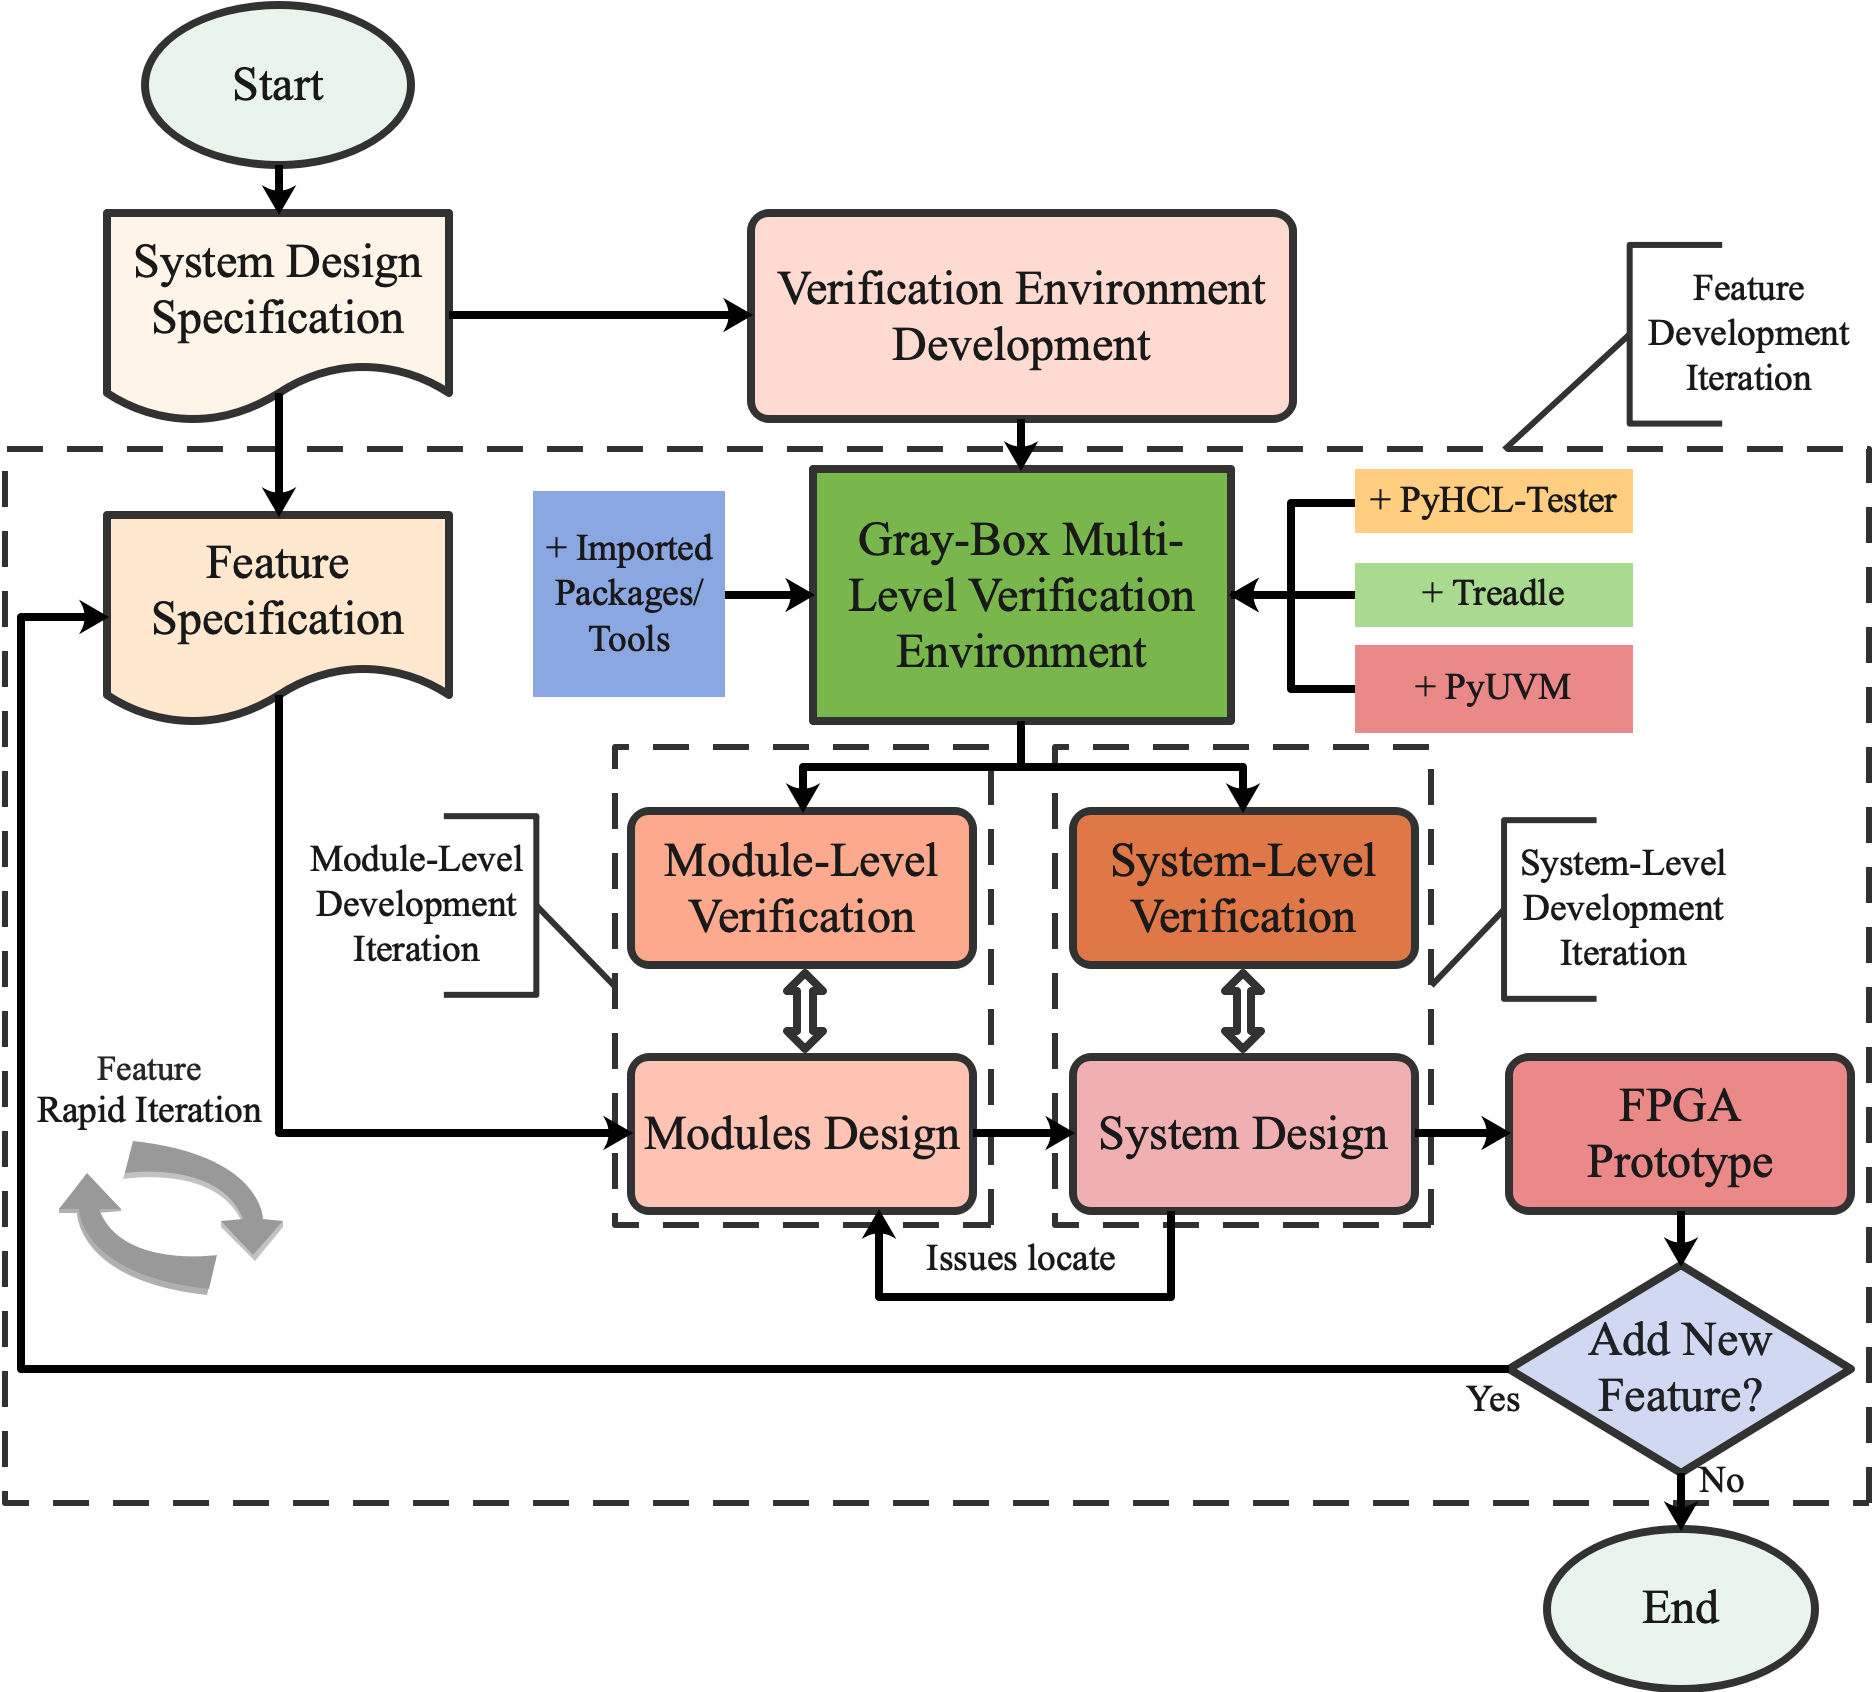
\includegraphics[width=0.95\textwidth]{Photos/process.png}
	\caption{基于PyHCL开发本文实现的RV32GCP微处理器内核FPGA原型的开发流程}
\end{figure}

在微处理器内核每个功能的开发周期当中,设计与验证时交织在一起进行的,而不是当设计全部完成后再进行验证,这可以大大缩短每个开发周期的时间,快速迭代完成FPGA原型开发并上板验证,以此来达到硬件敏捷设计的效果。在未来,PyHCL将会继续探究基于ASIC为后端的开发,并将本文所实现的RV32GCP内核完成ASIC后端的特定工艺流程。

综合全文的内容,本文所做的研究工作总结如下:

\begin{enumerate}
	\item 本文实现了基于RISC-V的RV32GCP微处理器内核,微处理器实现了基于“P”扩展指令集的低功耗SIMD指令,可以在保证低功耗的前提下提升嵌入式设备的运算能力,能够填补目前开源嵌入式RISC-V实现的空白。
	\item 本文实现的微处理器内核通过精心设计的小模块单元,如紧凑的预取缓冲区、4K全局两位饱和计数器分支预测器、分区加法器以及乘法器等在保证不会产生过多面积及功耗的同时,提高了微处理器的性能,使流水线整体CPI表现优异。
	\item 本文基于硬件敏捷设计思想设计了基于Python的全栈硬件开发框架PyHCL,其包含有完整的开发以及验证工具流。本文实现的RV32GCP微处理器即基于该框架设计并验证,并最终在FPGA目标后端成功部署并测试。
	\item PyHCL解决了绝大多数硬件生成框架的固有问题:设计与验证的分割,将设计与验证带到开发周期中交织同时进行,且整合了电路设计与验证的工具流,可以加快硬件开发周期的迭代速度。
	\item PyHCL实现的多级验证框架中提出的两种混合验证测试方法可以在保证仿真性能的前提下,结合各单个验证方法的优点,在模块级单元测试以及大规模集成测试中实现灰盒验证策略,加快单个开发周期中的验证流程。
\end{enumerate} %结论
	 %%%%%%%%%%%%%%%%%%%%%%%%%%%%%%%%%%%%%%%%%%%%%% bibtex参考文献设置  (原版)
%%	\bibliographystyle{scutthesis}
%%	\bibliography{F:/MyLibrary}
	%%%%%%%%%%%%%%%%%%%%%%%%%%%%%%%%%%%%%%%%%%%%%%
	%%%%%%%%%%%%%%%%%%%%%%%%%%%%%%%%%%%%%%%%%%%%%% biber参考文献设置	——by MCH
	\phantomsection % “目录”中的链接能正确跳转,需要添加 \phantomsection 否则点击参考文献会跳转到结论
	\addcontentsline{toc}{chapter}{参考文献}	%目录中添加参考文献
	\printbibliography	% 参考文献著录
 	%%%%%%%%%%%%%%%%%%%%%%%%%%%%%%%%%%%%%%%%%%%%%%
 	% 只有一个附录
% 	\include{appendix}
 	% 有多个附录
%	\include{appendix1} %附录1
%	\include{appendix2} %附录2
 	%%%%%%%%%%%%%%%%%%%
	\include{pub} %成果
	\chapter{致\texorpdfstring{\quad}{}谢}

三年的研究生生活在此即将划上句号,回首在华园的七年年时光,成功与挫折相伴,喜悦与伤感俱在。在七年的华园生活中,虽不能称得上别样的多姿多彩,但我还是能够说我度过了人生中最为充实,最为自由的时光。在此期间,家人的陪伴,老师的指导,同学的鼓励,都是我成长过程中不可或缺的一部分。
首先我要感谢我的导师赖晓铮老师,对我的毕业设计方面给予悉心的指导。老师不仅仅能够作为一个指导者的角色为我指引方向,还能作为一个合作者的角色经常与我讨论相关问题,并且能够让我自由的在喜欢的领域里尽情学习,更加激发了我浓厚的兴趣。同时,还感谢华园七年中我的所有任教老师,他们教给我许多的知识,为我打下了坚实的基础。同时,我还要感谢实验室的师兄师姐们,他们在毕业设计项目上对我帮助了许多。
然后我想感谢我的同学们,首先是我的舍友邓骏杰、王博和张德赋,我与他们相互陪伴的研究生学习生活,互相扶持走过了3年的时光。在我的研究生期间,赵森华,陈海康,范港平,赵伟杰等同学都带给了我快乐的时光,我也向他们学习了很多东西。我还要感谢我的好友邓楚钧以及吴卓桁同学,在我失落或者彷徨的时候给予我欢笑和鼓励。我衷心祝愿你们在未来能够脚踏实地,更进一步。
最后,我想感谢我的父母,他们始终是我最坚实的后盾,无论是生活还是学习上,他们都给我莫大的支持,感谢你们25年来对我的养育以及关爱,以及在我背后默默的付出。在未来的学习工作生活中,我希望我能够再接再厉,更近一步。

\begin{minipage}[t]{0.945\textwidth}%
	\begin{flushright}
		陈若晖\\
%		\today\\	% 自动时间
		2022年3月30日\\	%固定时间
		于华南理工大学
		\par\end{flushright}
\end{minipage}

 %致谢
\end{document}
